% \documentclass{report}
% \usepackage[utf8]{inputenc}
% \usepackage[brazil]{babel}

\documentclass[oneside,a4paper,12pt]{normas-utf-tex}

\usepackage{breakurl}
\usepackage[alf,abnt-emphasize=bf,bibjustif,recuo=0cm, abnt-etal-cite=2]{abntcite}
\usepackage[brazil]{babel}
\usepackage[utf8]{inputenc}
\usepackage{amsmath}
\usepackage{graphicx,subfig}
\usepackage{times}
\usepackage[plain]{fancyref}
\usepackage{float}
\usepackage{pdfpages}
\usepackage{enumitem}
\usepackage{longtable}
\usepackage{amssymb}
\usepackage{empheq}
\usepackage{bm}
\usepackage{setspace}
%\usepackage[loose]{units}

\newcommand{\unit}[1]{\ensuremath{\, \mathrm{~[#1]}}}



%%% Complemento para tabelas
\usepackage{booktabs, multirow}
\setlength{\heavyrulewidth}{0.1em}
\renewcommand{\toprule}{\midrule[\heavyrulewidth]}
\renewcommand{\arraystretch}{1.2}
%%%

\instituicao{Universidade Tecnológica Federal do Paraná}
\departamento{Departamento Acadêmico de Eletrônica}
\departamentodois{Departamento Acadêmico de Informática}
\programa{Curso de Engenharia de Computação}
\unidade{Oficina de Integração 3}

\titulo{\MakeUppercase{Mapeamento de ambientes com o robô Bellator}}
\documento{Monografia}

\autor{Luis Guilherme Machado Camargo}
\autordois{Pedro Alberto de Borba}
\autortres{Ricardo Farah}
\autorquatro{Stefan Campana Fuchs}
\autorcinco{Telmo Friesen}
\palavraschave{mapeamento de ambientes, robô, sensores infra-vermelho}
\keywords{environment mapping, robot, infrared sensors}

\cita{CAMARGO, L.G.M; BORBA, P.A.; FARAH, R.; FUCHS, S.C.; FRIESEN, T}

\comentario{\UTFPRdocumentodata\ apresentado à Unidade Curricular de \UTFPRunidadedata\ do \UTFPRprogramadata\ da \ABNTinstituicaodata\ como requisito parcial para aprovação.}

\local{Curitiba}
\data{\the\year}

\begin{document}

\capa
\folhaderosto

\begin{resumo}

Este projeto pretende utilizar o já existente robô Bellator para o propósito de mapeamento de ambientes. Por meio da utilização de sensores infra-vermelhos acoplados ao robô, medidas da distância de obstáculos em relação ao robô podem ser obtidas. Ao se marcar os pontos obtidos em um plano bidimensional, mapas de uma grande variedade de ambientes podem ser construídos.

\end{resumo}

\begin{abstract}

This project aims to use the already existing Bellator robot for the purpose of environment mapping. Using infrared sensors coupled to the robot, measurement of the distance of obstacles with reference to the robot can be acquired. By plotting these measurents onto a two dimensional grid, maps of a great variety of environments can be built.

\end{abstract}
\listadefiguras
\listadetabelas
\sumario
\chapter{Declaração do Escopo em Alto Nível}

O projeto apresentado neste documento trata-se do “Mapeamento de Ambientes com o robô Bellator” e é uma extensão do projeto “Bellator”. Ele teve sua última alteração em 2012 quando foi utilizado por Alexandre Jacques Marin, Júlio Cesar Nardelli Borges e Yuri Antin Wergrzn como plataforma de experimentos para o projeto final de conclusão de curso. O projeto para a disciplina de Oficina de Integração 3 será desenvolvido com base nesse robô. Na versão atual dele, está presente um conjunto de circuitos (com um microcontrolador) que gerencia as operações de baixo nível. Além disso, está presente um PC embarcado (executando o sistema Linux), que efetua as operações de alto nível.

A equipe deste projeto propõe modificar o robô Bellator para efetuar o mapeamento 2D de ambientes controlados como, por exemplo, labirintos construídos para fins de teste do robô. Posteriormente, em trabalhos futuros, ajustes finos poderão ser feitos para o uso em ambientes diversos, como escritórios, salas e quartos.

Na versão atual do Bellator, estão sendo utilizadas duas placas de circuito impresso – uma integrada com o microcontrolador e uma para a interface com os sensores – ambas ligadas por cabos entre si. Ao invés de produzir uma terceira placa para sensores adicionais (aspecto explicado mais à frente), o que aumentaria a quantidade de cabos, propõe-se desenvolver uma nova placa que realize a função de interface com todos os sensores e que seja acoplada ao microcontrolador. Este microcontrolador pode ser usado diretamente na forma encapsulada de circuito integrado (soldado diretamente na nova placa), ou integrado a um kit de desenvolvimento (acoplado como \textit{shield} na nova placa).

O sistema embarcado do robô será a placa de interface de sensores acoplada com o microcontrolador. Esse sistema realizará as funções de baixo nível, ou seja, leitura de sensores e controle do PWM dos motores. A estação base será um computador, provido de um software que efetua comunicação bidirecional com o robô. A estação será capaz de enviar comandos de movimentação (especificados manualmente pelo teclado) a ele, além de receber imagens da câmera e leituras dos sensores. No software, a partir das leituras dos sensores, será produzido um mapa em 2D simplificado do ambiente, com os obstáculos que forem detectados à medida que o robô andar, além do caminho estimado percorrido por ele. Protocolos de comunicação serão utilizados entre: circuito de baixo nível e o PC embarcado (através de porta serial), e entre PC embarcado e estação base (através de conexão WI-FI). A conexão entre a estação base e o robô deve ter um alcance de até 20 metros, e para isso a tecnologia WI-FI mostra-se adequada.

Um aspecto importante a ser notado é a exatidão e confiabilidade das medições de velocidade. No robô atual tem-se dois encoders, um para cada roda – a partir dos quais pode ser medida a velocidade e distância percorrida. Há certas desvantagens em utilizar essa abordagem, que são principalmente as questões de exatidão. Por exemplo, caso alguma roda escorregue, gire em falso ou sofra trepidações, as medições podem ser comprometidas – gerando distorções no mapa 2D. Por isso, propôe-se instalar novos sensores na carcaça do robô (acelerômetro e giroscópio) para adicionar maior confiabilidade nas medições do sistema – tendo em vista que esses sensores mensurarão o movimento real do robô e não somente o giro das rodas. Dessa forma, pode-se ter maior garantia de exatidão nos mapas gerados, levando-se em conta que a velocidade e posição do robô poderão ser melhor determinados. Especialmente em trabalhos futuros, se o robô for utilizado em ambientes acidentados ou em condições não ideais de terreno, esses sensores podem ser de grande valia – uma vez que nesses ambientes há maior chance da as rodas escorregarem, girarem em falso ou trepidarem.

\chapter{Especificação de Objetivos/Metas}
OBJETIVOS:

\begin{itemize}
  \item Implementar um software para comunicação de uma estação base (computador) com o robô, de forma que ela possa enviar comandos de movimentação ao robô, além de receber imagens da câmera e leituras dos sensores. Os comandos de movimentação (mover para frente, para trás, girar para esquerda/direita, parar) serão especificados por um utilizador humano através do teclado da estação base. 
  \item O meio de comunicação entre a estação base e o robô deverá ter alcance máximo de 20 m (se não houverem paredes ou obstáculos entre a estação base e o robô). Para isso a tecnologia WI-FI mostra-se adequada e, portanto, ela será utilizada.
  \item Inserir uma \textit{webcam} USB no robô, de modo que imagens do ambiente possam ser transmitidas à estação base. O propósito das imagens será unicamente permitir a visualização (pelo usuário da estação base, em tempo real) do ambiente no qual o robô está localizado. A câmera será conectada na porta USB do computador embarcado, e a transmissão de imagens será feita pelo canal Wi-Fi entre a estação base e o robô (o mesmo canal utilizado para a trasmissão de dados dos sensores e comandos de movimentação).
  \item Implementar, no software utilizado na estação base, a geração de uma mapa em 2D com o caminho estimado percorrido pelo robô e os obstáculos detectados pelo mesmo. Os obstáculos serão representados a partir dos pontos em que houve detecção pelos sensores.
  \item Instalar novos sensores (acelerômetro e giroscópio) para efetuar as medições de velocidade e posicionamento do robô com maior exatidão do que pode ser feito atualmente com os \textit{encoders}. Ambos os sensores serão posicionados na carcaça do robô. Caso discrepâncias de medição entre os \textit{encoders}, acelerômetro e giroscópio sejam detectadas (por exemplo, em caso de escorregamento de rodas), atenuações de erros poderão ser feitas no \textit{software} da estação base.
%  A velocidade e deslocamento lineares instantâneos serão determinados a partir da integração numérica da aceleração linear (cujas amostras serão obtidas com o acelerômetro em intervalos de tempo discretos). A velocidade e deslocamento angular instantâneos serão determinados a partir da integração numérica da aceleração angular (cujas amostras serão obtidas com o giroscópio em intervalos de tempo discretos). A posição atual do robô será gradualmente atualizada na representação do mapa à medida em que as amostras de aceleração linear e angular forem recebidas na estação base.
  \item Desenvolver uma placa de circuito impresso que realize a função de interface com os sensores e que seja acoplada ao microcontroldador. Este microcontrolador pode ser usado diretamente na forma encapsulada de circuito integrado (sendo soldado diretamente na nova placa) ou integrado a um kit de desenvolvimento (acoplado como \textit{shield} na nova placa).
  \item Em caso de falha de comunicação entre o robô e a estação base, o robô deverá permanecer parado e aguardando a conexão ser reestabelecida.
\end{itemize}

METAS:
\begin{itemize}
  \item Concluir o trabalho com um prazo máximo de até 10 semanas. Incluindo planejamento, desenvolvimento, teste e documentação. 
  \item Não ultrapassar o orçamento inicial e o orçamento limite, detalhados posteriormente.
Desenvolver e manter um cronograma para que todos os integrantes da equipe tenham a possibilidade de trabalhar com o projeto sem causar prejuízos às outras matérias do curso.
\end{itemize}

\chapter{Premissas e restrições}
PREMISSAS:
\begin{itemize}
  \item Por ser utilizado o robô Bellator que já provém de trabalhos anteriores, infere-se que não haverá necessidade de haver gastos de tempo com consertos de equipamentos defeituosos ou correções de bugs no código fonte. Parte-se do pressuposto que o robô funciona de acordo com o que foi exposto nos relatórios anteriores.
  \item O robô é capaz de detectar obstáculos (paredes e objetos fixos de tamanho considerável que sejam maiores que ele) através dos sensores. A distância mínima para detecção é de 20cm e a máxima de 150cm.
  \item O robô é capaz de locomover-se em terrenos planos, não acidentados e em condições não severas.
  \item Pressupõe-se que o robô será disponibilizado para a equipe sem custos.
Podem ser utilizados os equipamentos e componentes diversos que já estejam disponíveis, com o objetivo de redução de custos.
\end{itemize}

RESTRIÇÕES:
\begin{itemize}
  \item O tempo disponível para a equipe é limitado, portanto muita atenção será dada às fases de planejamento e testes iniciais de modo a evitar imprevistos.
  \item A equipe deverá seguir um calendário previamente estabelecido, tendo o objetivo de evitar atrasos.
  \item O robô não será capaz de se locomover em terrenos acidentados, em escadas e similares.
  \item O robô não transportará cargas.
  \item O robô e a estação base não executarão algoritmos de roteamento ou mapeamento autônomo de ambientes. O controle de movimentação deverá ser feito obrigatoriamente por um usuário humano junto à estação base. O robô não fará nenhuma movimentação automática em caso de falha de conexão. Ele permanecerá parado aguardando a conexão ser reestabelecida.
  \item O robô e a estação base não serão capazes de efetuar mapeamento 3D.
  \item O robô e a estação base não irão armazenar automaticamente fotos ou vídeos dos ambientes explorados.
  \item O robô e o ponto de acesso WI-FI da estação base devem estar a uma distância máxima de 20 metros um do outro (supondo que não hajam paredes ou obstáculos). Caso contrário, não haverá garantias de que a comunicação entre a estação base e o robô seja funcional.
  \item Não serão usadas imagens do ambiente para a geração dos mapas.
  \item Os obstáculos não serão identificados quanto ao tipo ou forma. Serão apenas detectados pela sua presença.
\end{itemize}

\chapter{Designação do Gerente e da Equipe}
A equipe consiste de cinco integrantes. O gerente ocupou esta função com consentimento de todos.

GERENTE:
\begin{itemize}
  \item Luis Guilherme Machado Camargo.
\end{itemize}
COLABORADORES:	
\begin{itemize}
  \item Pedro Alberto de Borba, Ricardo Farah, Stefan Campana Fuchs, Telmo Friesen.
\end{itemize}


\chapter{Responsabilidades e Autoridade do Gerente}
\begin{itemize}
  \item O gerente poderá efetuar os gastos de valores estimados na análise de custos sempre informando os outros integrantes da equipe. Caso exista a necessidade de utilizar os valores previstos na margem de erro do orçamento, toda equipe deverá ser notificada e informada dos motivos.
  \item O gerente poderá liberar verba para um membro da equipe caso seja necessário. O gerente deverá registrar o valor gasto, o produto/serviço requerido e a pessoa que solicitou os recursos. Além disso, deve informar os outros membros da equipe sobre o fato.
  \item O gerente deverá atualizar o planejamento do projeto conforme exista a necessidade de mudanças, além de informar a equipe sobre o fato.
  \item O gerente deverá garantir que o projeto esteja progredindo conforme planejado.
  \item O gerente sempre deverá se portar educadamente a todos os membros da equipe.
  \item O gerente não tem poderes para efetuar a demissão de ninguém.
  \item O gerente tem o poder de tomar decisões em nome da equipe, preferencialmente considerando a opinião dos outros membros.
  \item O gerente tem o poder de intervir em qualquer conflito que ocorra internamente ou externamente à equipe.
  \item O gerente deve intermediar as reuniões da equipe.
  \item O gerente deve controlar as horas de trabalho da equipe e o cumprimento de prazos.
  \item O gerente deve falar em nome da equipe quando não for possível que toda ela o faça.
  \item O gerente deverá cobrar a escrita de documentação por todos os integrantes da equipe, de acordo com o que for desenvolvido por cada um.
\end{itemize}

%Neste capítulo estão expostos os riscos previstos para o projeto.

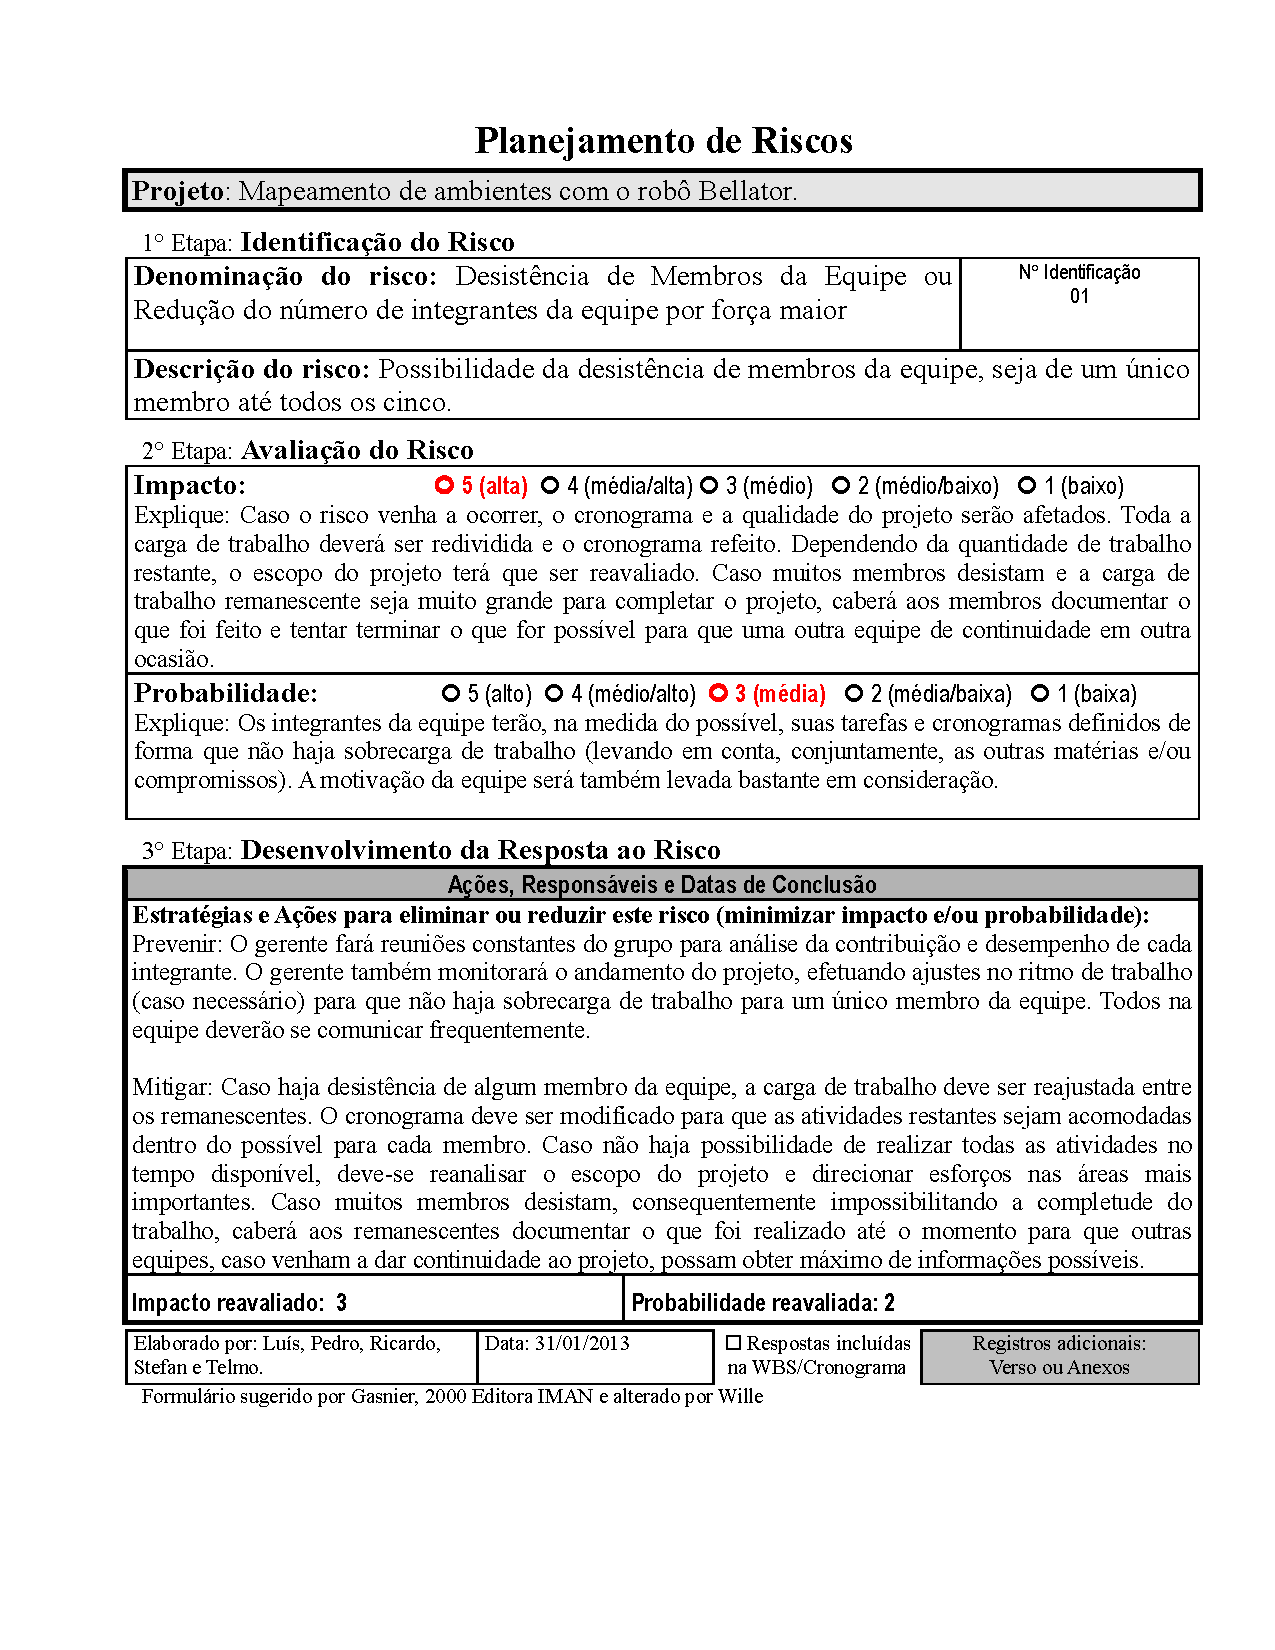
\includepdf[pages=1,scale=0.5, pagecommand=\chapter{Planejamento de riscos}]{Planejamento_de_Riscos_v3.pdf}
\includepdf[pages=2-9, pagecommand=]{Planejamento_de_Riscos_v3.pdf}

\chapter{Trabalhos correlatos}

O mapeamento de ambientes realizado por robôs visa ao desenvolvimento de software e hardware que permitam a construção de um mapa a partir de dados captados por um ou mais sensores. Há diversas tecnologias que podem ser empregadas para alcançar tal objetivo, como o processamento de digital de imagens captadas de uma câmera ou a utilização de sensores de proximidade tais como sensores de ultrassom ou sensores de ondas eletromagnéticas.

Esta última opção mostra-se bastante adequada para a maioria dos projetos, pois garante uma medição satisfatória da distância de objetos próximos ao robô a um custo não muito elevado. Um dos sensores mais populares deste tipo é o sensor de proximidade de infravermelho. Quando integrado ao robô permite a obtenção várias medidas discretas da distância do robô a objetos, um dos elementos básicos que permitem a geração do mapa do ambiente.

\subsection{PatrolBot}
O PatrolBot \cite{patrol_bot} é um robô configurável desenvolvido com interesses comerciais. Ele pode criar uma planta do interior de construções. Utilizando a tecnologia WI-FI ele pode ser controlado remotamente ou se movimentar de forma autônoma, sendo apenas monitorado pela estação base. Tal comunicação é feita por Wi-Fi.

Ele permite a inclusão de acessórios adicionais tais como uma câmera e microfones que permitirão ver e ouvir o que se passa no ambiente que está sendo mapeado. Há diversos outros periféricos que podem ser incluídos no robô, que também oferece a opção de ser programado, por meio de um kit de desenvolvimento próprio.

\subsection{Sistema de mapeamento robótico bidimensional por infravermelho}

Nesta implementação \cite{wii}, um telêmetro infravermelho é utilizado para obter a distância de objetos próximos. A câmera infravermelha do Nintendo Wii é utilizada juntamente com sinalizadores (LEDs) para triangular a posição do robô e sua direção.

Como hardware, foram utilizados: um Arduino Mini Pro, um cartão microSD, telêmetro inframervelho, câmera do Wii. Não há comunicação em tempo real com a estação base. Isto significa que os dados são obtidos e armazenados no cartão microSD. Para leitura, o cartão deve ser inserido em um computador e, então, carregado na estação base. Os resultados são visualizados em um arquivo textual simples, no qual a letra "O" simboliza a posição do robô e a letra "X" os obtáculos detectados.

\chapter{Análise tecnológica}
Nesta seção está explicitada, primeiramente, uma visão geral do projeto. Em seguida, há uma discussão detalhada a respeito dos requisitos de cada parte fundamental -- estação base, sistema de comunicação e sistema embarcado. Por fim há uma enumeração das alternativas tecnológicas pesquisadas e das escolhidas para o preenchimento dos requisitos.

\section{Visão geral do projeto}

O projeto, de um ponto de vista geral, consiste em um robô controlado manualmente e que seja capaz de efetuar mapeamento em duas dimensões de ambientes. Um usuário humano monitorará e controlará um computador -- a estação base -- a partir do qual poderão ser enviados comandos de movimentação, via teclado, ao robô. Informações sobre o posicionamento do robô e dos obstáculos detectados por ele serão recebidas na estação base em tempo real. Imagens instantâneas de uma câmera posicionada no robô -- aspecto explicado mais à frente -- poderão ser visualizadas pelo utilizador.

O sistema de comunicação deverá ter, ao menos, alcance de 20 metros sem fios. Visto que toda a comunicação entre a estação base e o sistema embarcado será feita por um único canal, a velocidade e o tipo de fluxo de transmissão de dados devem ser adequados para, simultaneamente, o envio de comandos de movimentação ao robô, recebimento de dados de leituras de sensores e recebimento de imagens da câmera.

O sistema embarcado é constituído, em suma, pelo robô. Ele deve ser capaz de se mover para frente e para trás e girar para a esquerda e direita. A visualização em tempo real do ambiente pelo utilizador, com o objetivo de facilitar o controle de movimentação manual, poderá ser feita através de imagens instantâneas geradas por uma câmera fixa instalada no robô. 

O robô deve ser capaz de obter dados para cálculos (na estação base) de sua velocidade e deslocamento. Um aspecto desejável em relação a isso é a atenuação de erros em decorrência de escorregamento, giros em falso ou trepidação de rodas, visando, dessa forma, a utilização futura do robô em condições não ideais de terreno. Obstáculos próximos -- em uma distância mínima de 30 cm e máxima de 150 cm -- devem ser detectados de modo a possibilitar a confecção de um mapa 2D em tempo real na estação base.

\section{Requisitos}


\subsection{Estação base}
%
%TODO verificar objetivos do projeto
Esta seção descreve os requisitos da estação base, que foram elaborados de forma a satisfazer os objetivos do projeto.

\begin{itemize} %-------------------

  \item O \textit{software} será executado em um computador pessoal.
    \begin{itemize}
%      \item O computador deverá possuir recursos de \textit{hardware} comparável aos padrões atuais (pelo menos 2GB de memória RAM DDR2 ou melhor e processador \textit{dual-core}).
      \item O \textit{software} deverá ser multiplataforma, ou seja, executar em diferentes sistemas operacionais (ao menos Linux e Windows).
      \item Preferencialmente bibliotecas e ferramentas livres (e gratuitas) deverão ser utilizadas no desenvolvimento do \textit{software}.
    \end{itemize}

  \item O software deve possuir uma interface gráfica.
    \begin{itemize}
      \item Um utilizador, através da interface gráfica, será capaz de controlar o robô enviando comandos de movimentação (especificados pelo teclado). 
      \item O usuário receberá a imagem em tempo real (preferencialmente com atrasos não muito consideráveis) de uma câmera fixa instalada no robô. 
      \item Os dados instantâneos de velocidade e posição do robô serão mostrados ao usuário na interface gráfica.
      \item Um mapa 2D do caminho percorrido e dos obstáculos detectados pelo robô será gerado, na interface gráfica, à medida em que o robô se movimentar. O caminho percorrido por ele será representado por pontos interpolados que demonstrem visulamente a trilha percorrida por ele. Os obstáculos serão representados por pontos, não interpolados, nos quais houve detecção de objetos pelos sensores. Todos os pontos representados no mapa serão gerados a partir de amostras em intervalos de tempo discretos de leituras de sensores do robô.
      \item O mapa 2D gerado na interface poderá ser salvo em um arquivo, podendo ser posteriormente carregado.
    \end{itemize}

\end{itemize} %----------------------



\subsection{Sistema de comunicação}
Esta seção descreve os requisitos do sistema de comunicação entre a estação base e o sistema embarcado.

\begin{itemize} %----------------------

  \item Distância entre robô e estação base.
    \begin{itemize}
      \item O sistema de comunicação deve possuir alcance máximo de 20 metros, de modo que ambientes de tamanho razoável possam ser mapeados.
    \end{itemize}

  \item Velocidade e direção do fluxo de transmissão de dados.
    \begin{itemize}
      \item A velocidade de transmissão do canal de comunicação deve ser suficiente para o envio de comandos de movimentação ao robô, recebimento de dados de leituras de sensores e recebimento de imagens da câmera em tempo real -- visto que toda a comunicação entre a estação base e o sistema embarcado será feita por um único canal.
      \item O fluxo de dados deve ser bidirecional (\textit{full-duplex}).
    \end{itemize}

\end{itemize} %----------------------



\subsection{Sistema embarcado}
Esta seção descreve os requisitos do sistema embarcado (robô).

\begin{itemize} %----------------------

  \item Movimentação do robô.
    \begin{itemize}
      \item O robô deve ser capaz de mover-se para frente, para trás e girar para a esquerda e direita em velocidades baixas.
%      \item A velocidade de movimentação pode ser relativamente pequena. %%TODO verificar velocidade do bellator nas monografias anteriores
    \end{itemize}

  \item Controle de posicionamento e velocidade.
    \begin{itemize}
      \item O robô deve ser capaz de obter dados que permitam calcular sua velocidade (linear e angular) e posição (deslocamento e rotação), enviando-os à estação base.
    \end{itemize}

  \item Detecção de obstáculos.
    \begin{itemize}
      \item O robô deverá ser capaz de detectar obstáculos próximos -- com distância de no mínimo 30 cm e no máximo 150 cm -- localizados ao seu redor, determinando a distância de cada objeto detectado.
    \end{itemize}

\end{itemize} %----------------------


\section{Análise de opções tecnológicas}

Nesta seção está apresentada a análise das opções tecnológicas plausíveis para o atendimento dos requisitos. As alternativas pesquisadas e as escolhidas para cada parte do projeto estão explicitadas a seguir.

\subsection{Estação base}

As alternativas pesquisadas para a estação base estão apresentadas nesta subseção.

\subsubsection{Biblioteca para desenhos 2D}
\label{subsec:alternativas_desenho}

Tendo em vista que um dos requisitos é a geração de um mapa em duas dimensões na estação base, deve-se escolher uma biblioteca que permita realizar o desenho de formas geométricas diversas e que possa ser integrada facilmente à interface gráfica. Ela deve também possuir meios simples de obter informações do mouse e teclado, para interatividade com o usuário. 

Uma biblioteca interessante disponível em Java que possui o recurso de produzir desenhos dinâmicos (e integrá-los a interfaces gráficas) é o Processing \cite{processing}, \textit{open-source}. Essa biblioteca foi a principal encontrada que seria capaz de satisfazer as necessidades de desenho do mapa 2D de forma simples. Por possuir inúmeras funções de desenho em alto nível, o trabalho de renderização dos gráficos seria consideravelmente simplificado. Além disso, na biblioteca existem recursos que permitem o recebimento de informações de posicionamento do mouse e de comandos do teclado. Por ser constituído basicamente de um \textit{Applet} Java, o Processing pode facilmente ser integrado a componentes do Swing -- biblioteca de interface gráfica (GUI) do Java.


Outra biblioteca para a confecção de desenhos em 2D é o Cairo \cite{cairo}, que é \textit{open-source}, disponível nas linguagens C e C++. Ele possui recursos em alto nível para renderização de formas e interação com o usuário, assim como o Processing. Nos aspectos gerais as duas ferramentas são muito semelhantes. A integração do Cairo com a interface gráfica, porém, é dependente na biblioteca externa de GUI utilizada para tal.

Um aspecto importante a notar é que ambas as bibliotecas foram desenvolvidas e otimizadas para terem bom desempenho em máquinas atuais -- o que é desejável tendo em vista os requisitos. Na Tabela \ref{tab:alternativas_desenho} está presente uma comparação entre as duas bibliotecas.


\begin{table}[h]
  \caption{Comparação entre Bibliotecas para desenhos 2D.}
  \centering
  \begin{tabular}{p{6cm}|p{4cm}p{4cm}}
    \toprule
    \textbf{Característica} & \textbf{Cairo} & \textbf{Processing} \\
    \midrule
    Linguagem de programação & C e C++ & Java \\
    \hline
    Integração com interface gráfica & Sim (depende da biblioteca de GUI utilizada) & Sim (na biblioteca Swing do Java) \\
    \hline
    Ferramentas de interação com o usuário & Sim & Sim \\
    \bottomrule
  \end{tabular}
  \label{tab:alternativas_desenho}
\end{table}

A escolha da biblioteca de desenhos foi feita em conjunto com a escolha de linguagem de programação. A biblioteca escolhida, dentre as duas opções, foi o Processing, visto que a integração a interfaces gráficas do Java é muito simples. 

\subsubsection{Linguagem de programação}

Nessa etapa de avaliação das opções, a escolha de uma boa linguagem de programação que atenda aos requisitos é fundamental. Abaixo está presente uma lista dos aspectos desejáveis da linguagem:

\begin{itemize}
  \item Deve ser multiplataforma (ao menos compatível com Linux e Windows sem muitas modificações);
  \item Deve possuir orientação a objetos;
  \item Deve possuir recursos multiplataforma e \textit{open-source} para o desenvolvimento de interfaces gráficas;
  \item Deve ter a disponibilidade de ferramentas \textit{open-source} e multiplataforma para a criação visual da interface gráfica, dessa forma agilizando o processo de desenvolvimento;
  \item Deve possuir recursos, integrados ou em bibliotecas \textit{open-source}, para o desenvolvimento de desenhos dinâmicos (para a geração do mapa 2D). Os desenhos devem ser facilmente integráveis à interface gráfica.
\end{itemize}


Abaixo está presente uma descrição das duas linguagens, o C++ e Java, atualmente utilizadas em inúmeras aplicações, e que são potenciais alternativas ao projeto. A Tabela \ref{tab:alternativas_linguagens} sumariza os recursos de cada uma.

\textbf{Java}

O Java \cite{java} é uma linguagem concebida de início como sendo orientada a objetos. A maneira com que é feita a compilação e execução do código permite que muito facilmente programas sejam rodados em diferentes plataformas (Linux, Windows, Mac, entre outros). O processo de compilação do código gera os chamados \textit{bytecodes}, que são instruções a serem interpretadas pela \textit{Java Virtual Machine} (JVM). A grande vantagem é que o JVM possui disponibilidade multiplataforma, e a manutenção pelos desenvolvedores é frequente.

Há disponibilidade, na API do Java, da biblioteca Swing -- que contém recursos completos para a criação de interfaces gráficas (GUI) interativas. Existem ferramentas visuais de código aberto que consideravelmente agilizam o processo de desenvolvimento de interfaces Swing, entre elas o NetBeans \cite{netbeans} e o Eclipse \cite{eclipse}, através de plugins ou extensões. 

Para o preenchimento do requisito de confecção de desenhos em 2D com integração à interface gráfica, a biblioteca do Processing (explicada anteriormente na Subseção \ref{subsec:alternativas_desenho}) está disponível nessa linguagem.


\textbf{C++}

O C++ é uma linguagem orientada a objetos, que foi desenvolvida a partir da linguagem C. A compilação de código no C++ deve ser feita especificamente para cada plataforma em que os programas desenvolvidos forem utilizados. De uma perspectiva prática, certas seções de código frequentemente necessitam de adaptações manuais para cada plataforma e sistema operacional, o que gera retrabalho e gastos de tempo adicionais. 

Recursos para desenvolvimento visual de interfaces gráficas estão disponíveis através de bibliotecas e ferramentas externas. O C++ não possui recursos de interface gráfica na própria API. Deve-se notar que esse é um aspecto que adiciona complexidade ao portar programas entre diferentes sistemas. 

Para a confecção de desenhos 2D e incorporação dos mesmos à interface gráfica, a biblioteca Cairo (explicada anteriormente na Subseção \ref{subsec:alternativas_desenho}) pode ser utilizada com essa linguagem. A possibilidade de haver integração com a interface, porém, é dependente da biblioteca de GUI utilizada.


\textbf{Escolha da equipe:} O Java foi a linguagem escolhida para o desenvolvimento do \textit{software} da estação base, uma vez que preenche satisfatoriamente os requisitos do projeto. A escolha do Java foi feita em conjunto com a escolha da biblioteca do Processing. Notavelmente, há a facilidade em portar, sem adaptações, programas para diferentes plataformas, processo este que é mais complexo no C++.  Com relação ao quesito de desempenho em computadores atuais, a linguagem escolhida é satisfatória, visto que há manutenção constante da implementação das bibliotecas e da máquina virtual do Java pelos desenvolvedores -- que buscam, entre outros aspectos, otimizar a linguagem para tecnologias atuais.

\begin{table}[h]
  \caption{Comparação entre linguagens de programação.}
  \centering
  \begin{tabular}{p{6cm}|p{4cm}p{4cm}}
    \toprule
    \textbf{Característica} & \textbf{C++} & \textbf{Java} \\
    \hline
    Multiplataforma (Linux e Windows) & Sim (com adaptação) & Sim (sem adaptação) \\
    \hline
    Orientação a objetos & Sim & Sim \\
    \hline
    Recursos multi-plataforma e \textit{open-source} para desenvolvimento de interface gráfica (GUI) & Sim (com bibliotecas externas) & Sim (integrado à API da linguagem) \\
    \hline
    Ferramentas \textit{open-source} e multiplataforma para criação visual de interface gráfica & Sim (ferramentas externas) & Sim (ferramentas externas) \\
    \hline
    Recursos \textit{open-source} para desenvolvimento de desenhos dinâmicos, facilmente integráveis à interface gráfica & Sim (biblitoeca externa, integração à interface gráfica dependente da GUI utilizada) & Sim (biblioteca externa) \\
    \bottomrule
  \end{tabular}
  \label{tab:alternativas_linguagens}
\end{table}



\subsection{Sistema de comunicação}

Na Tabela \ref{tab:alternativas_comunicacao} está presente uma comparação entre diferentes tecnologias de comunicação sem fios. O Wi-Fi é o recurso mais atrativo em todos os aspectos que foram comparados, preenchendo satisfatoriamente os requisitos do sistema de comunicação. Sua velocidade e alcance são suficientes para satisfazer as necessidades, e o fluxo de dados pode ser \textit{full-duplex}. Notavelmente, o Wi-Fi é o único sistema comparado que oferece a possibilidade (com simplicidade) de uso do protocolo TCP -- o que é um requisito importante para o desenvolvimento ágil e satisfatório do projeto.


\begin{table}[h]
  \caption{Comparação entre tecnologias de comunicação sem fios.}
  \centering
  \begin{tabular}{p{4.5cm}|p{3cm}p{4cm}p{2cm}}
    \toprule
    \textbf{Característica} & \textbf{802.11g (Wi-Fi)} & \multicolumn{1}{l}{\textbf{Rádio Frequência (RF)}} & \textbf{Bluetooth}  \\
    \hline
    Distância máxima de alcance & 50-100 metros  & 30-100 metros & 10 metros \\
    \hline
    Velocidade de transmissão máxima & 54 Mbits/s & 2 Mbits/s & 1 Mbits/s \\
    \hline
    Fluxo de dados \textit{full-duplex} & Sim & Sim & Sim \\
    \hline
    Possibilidade e simplicidade de uso de TCP & Sim & Não & Não \\
    \bottomrule
  \end{tabular}
  \label{tab:alternativas_comunicacao}
\end{table}



\subsection{Sistema embarcado}

Nesta seção apresentamos as alternativas pesquisadas para o sistema embarcado, levando em conta os requisitos já apresentados anteriormente.

\subsubsection{Movimentação do robô}

O sistema de movimentação do robô, incluindo motores, acionadores, drivers de potência e rodas não foram pesquisados pois já estão implementados no robô e atendem aos requisitos especificados nas seções anteriores. Sendo assim utilizaremos um chassi de 40 cm de largura por 50 cm de comprimento, duas rodas de tração e uma roda guia. As rodas de tração estão dispostas na parte posterior do robô, possuindo 20 cm de diâmetro e 4 cm de largura. O chassi está equipado com 2 motores Bosch FPG 12V, 2 baterias Unybatt 12V-7,2 Ampére-hora e duas pontes H L298 \cite{bellator_2012}. A disposição dos itens no robô pode ser vista na figura \ref{fig:disposicao_bellator_2012}.

\begin{figure}[H]
\centering
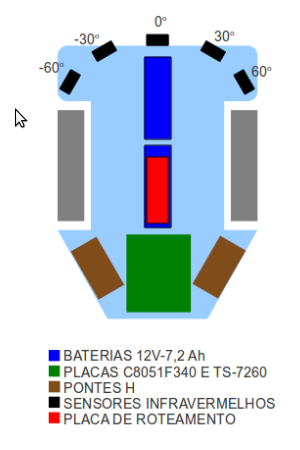
\includegraphics[width=0.4\textwidth]{./figuras/disposicao-robo.png}
\caption[Disposição dos itens no robô]{Disposição dos itens no robô}
\fonte{\cite{bellator_2012}}
\label{fig:disposicao_bellator_2012}
\end{figure}

\subsubsection{Odometria}

Para a obtenção da direção e sentido do movimento do robô, assim como aceleração, velocidade e posição, pode-se optar por diversos tipos de tecnologias ou pela associação delas. Abaixo descrevemos as principais delas.

\begin{itemize}
  \item \textbf{Encoder:} Ligado ao eixo da roda do robô, conta a quantidade de voltas dadas pela roda. Permite assim calcular a distancia percorrida pelo robô. Caso sejam conectados dois encoders, um em cada roda, podemos obter também a direção do movimento pela diferença entre a contagem de voltas de cada roda.
  \item \textbf{GPS:} Utiliza sinais de satélites para obter as coordenadas geográficas do robô. A direção e o sentido podem ser obtidos pela comparação das leituras com as anteriores.
  \item 	\textbf{Acelerômetro:} pode utilizar a tecnologia chamada \textbf{MEMS} para medir a aceleração sofrida pelo componente.
  \item 	\textbf{Giroscópio:} pode utilizar a tecnologia chamada \textbf{MEMS} para medir a aceleração angular sofrida pelo componente.
  \item 	\textbf{Bussola:} Utiliza os campos magnéticos da terra para obter a direção com relação aos polos magnéticos da terra.
\end{itemize}

A seguir, na tabela \ref{tab:alternativas_tecnologias_odometria}, comparamos as tecnologias apresentadas anteriormente. 

\begin{table}[h]
  \caption{Comparação entre tecnologias para odometria.}
  \centering
  \begin{tabular}{p{3cm}|p{2.2cm}p{1.7cm}p{2.2cm}p{2.2cm}p{2.2cm}}
    \toprule
    \textbf{Característica} & \textbf{Encoder} & \textbf{GPS} & \textbf{Acelerômetro} & \textbf{Giroscópio} & \textbf{Bussola} \\
    \hline
    Sujeito a influencias externas & Deslizamentos & Não & Não & Não & Campo magnético dos motores \\
    \hline
    Ambiente de operação & Interno / Externo & Externo & Interno / Externo & Interno / Externo & Interno / Externo \\
    \hline
    Posicionamento & Relativo & Absoluto & Relativo & Relativo & Relativo \\
    \bottomrule
  \end{tabular}
  \label{tab:alternativas_tecnologias_odometria}
\end{table}

Com base no comparativo da tabela \ref{tab:alternativas_tecnologias_odometria} optamos por utilizar um acelerômetro em conjunto com um giroscópio para obter os dados para odometria. Encoders estão sujeitos a erros causados por deslizamento nas rodas, GPS apenas funciona em ambientes externos e a bussola pode ser influenciada pelo campo magnético dos motores. Como o robô já apresenta encoders instalado, utilizaremos também os dois encoders, possibilitando assim aumentar a precisão e confiabilidade dos dados de odometrias.
Justificada nossa escolha por acelerômetros e giroscópios, na tabela \ref{tab:alternativas_componentes_odometria} fazemos um comparativo entre as opções de menor custo disponíveis no mercado. Listamos na tabela apenas as alternativas que possuem placas de desenvolvimento pois acelerômetros e giroscópios são geralmente são vendidos em encapsulamento LGA, os quais são de difícil soldagem.

\begin{table}[h]
  \caption{Comparação entre acelerômetros/giroscópios para odometria.}
  \centering
  \begin{tabular}{p{2.4cm}|p{3cm}p{0.8cm}p{1.4cm}p{1.8cm}p{1.7cm}p{1.3cm}}
    \toprule
    \textbf{Modelo} & \textbf{Fabricante} & \textbf{Acel.} & \textbf{Giro.} & \textbf{Faixa} & \textbf{Interface} & \textbf{Preço} \\
    \hline
    STEVAL-MKI009V1	& STMicroeletronics & 3x	& - & $ \pm 2g / \pm6g $ & I2c / SPI & \$23.94 \\
    \hline
	ATAVRSBIN1 & Atmel & 1x & - & - & I2c & \$26.25 \\
	\hline
	KIT3803 MMA7660FC & Freescale & 3x & - & $ \pm 1.5g $ & I2C & 	\$35.0 \\
	\hline
	ATAVRSBIN1 & Atmel & - & 1x & & I2C & \$26.25 \\
	\hline
	MPU-6050	 & IvenSense & 3x & 3x & $ \pm 2g / \pm 4g $ $ \pm 250 ^{o}/seg /$ $ \pm 500 ^{o}/seg $ & I2C & \$8.78 \\
    \hline
	MKI086V1	 & STMicroeletronics & 1x & $ \pm 30^{o}/seg $ & Analog & & \$31.50 \\
	\hline
	STEVAL-MKI094V1 & STMicroeletronics & - & 3x & $ \pm 400^{o}/seg $ & Analog & \$31.50 \\
	\hline
	ATAVRSBIN1 & Atmel & 1x & 1x & & I2C & \$26.25 \\
	\hline
	DM240316	 & Zena & 3x & 3x & 	& RF & \$99.99 \\
    \bottomrule
  \end{tabular}
  \label{tab:alternativas_componentes_odometria}
\end{table}

\textbf{MPU-6050}

Com base na tabela \ref{tab:alternativas_componentes_odometria} escolhemos o modelo MPU-6050 da IvenSense principalmente devido ao seu baixo custo: \$8.78. Este modelo possui um acelerômetro de 3 eixos, um giroscópio e 3 eixos e entradas para uma bussola externa integrados em um único chip \cite{mpu6050}. A faixa de operação para o acelerômetro é de $ \pm 2g ou \pm 4g $ e para o giroscópio é de $ \pm 250 ^{o}/seg $ ou $ \pm 500 ^{o}/seg $. A sensibilidade do acelerômetro é de $ 16384 LSB/g $ e $ 8192 LSB/g $. A sensibilidade do giroscópio é de $ 131 LSB/ ^{o} / seg $ e $ 65.5 LSB/ ^{o} / seg $. A interface de comunicação do módulo suporta o protocolo I2C. O módulo contendo o chip MPU-6050 e alguns componentes necessários para seu funcionamento pode ser visto na figura \ref{fig:mpu6050}.

\begin{figure}[H]
\centering
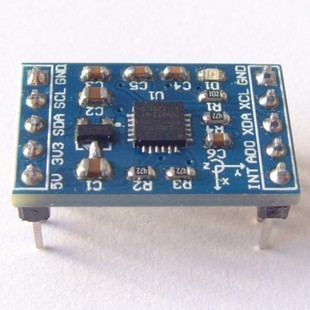
\includegraphics[width=0.4\textwidth]{./figuras/mpu6050.JPG}
\caption[Placa de desenvolvimento contendo o chip MPU-6050]{Placa de desenvolvimento contendo o chip MPU-6050}
\fonte{\cite{mpu6050}}
\label{fig:mpu6050}
\end{figure}

\textbf{Encoder Optico HEDS-9700}

Como já foi dito, utilizaremos também os encoders já existentes no robô. O robô está equipado com dois encoders HEDS-9700.
Esses encoders geram em sua saída uma onda quadrada à medida em que o encoder é rotacionado, sendo 1800 pulsos gerados em uma rotação \cite{heds9700}. A forma de onda da saída do encoder pode ser vista na figura \ref{fig:heds9700}. Podemos ver na figura que o encoder possui duas saidas, A e B com defasamento $\phi$ entre elas. Com as duas saídas podemos determinar o sentido de rotação. Porém na implementação existente esse recurso não é utilizado.

\begin{figure}[H]
\centering
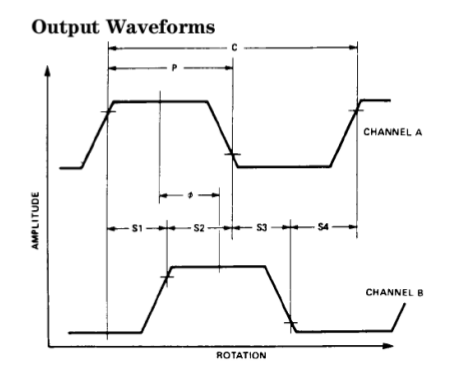
\includegraphics[width=0.6\textwidth]{./figuras/heds9700.png}
\caption[Forma de onda de saída do encoder]{Forma de onda de saída do encoder}
\fonte{\cite{heds9700}}
\label{fig:heds9700}
\end{figure}

\subsubsection{Detecção de obstáculos}

\textbf{Sensor de proximidade Infra Vermelho IR 2Y0A02F98}

A detecção de obstáculos, que é um requisito deste robô, será atendido pelos sensores de Infra vermelho já existentes no robô. Logo serão utilizados sensores IR 2Y0A02F98 \cite{ir_sensor}. Este modelo é pouco influenciado pelas cores dos objetos detectados devido ao método de medição baseado em triangulação. Na figura \ref{fig:ir_sensor_response} podemos ver isso. A linha tracejada é a resposta para reflexão em um papel cinza e a linha contínua é a resposta para reflexão em um papel branco.

\begin{figure}[H]
\centering
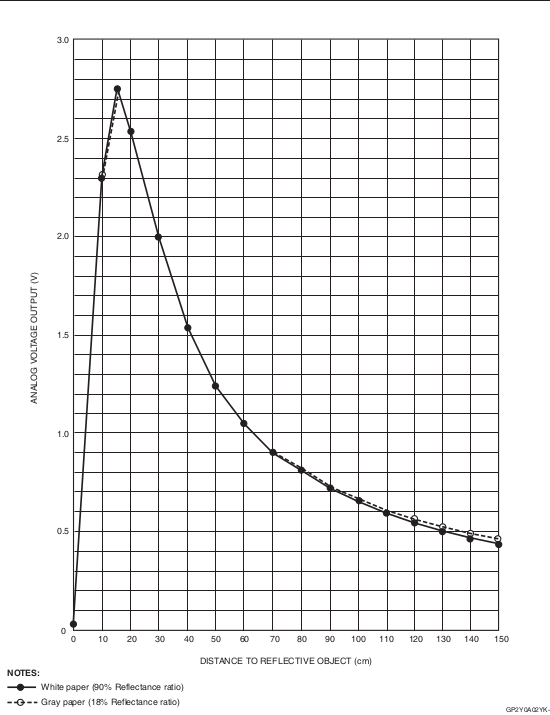
\includegraphics[width=1\textwidth]{./figuras/ir-sensor-response.png}
\caption[Curva de resposta do encoder]{Curva de resposta do encoder}
\fonte{\cite{ir_sensor}}
\label{fig:ir_sensor_response}
\end{figure}

\subsubsection{Microcontrolador}

A interface entre os sensores, atuadores e a placa TS-7260 já existente no robô \cite{bellator_2012} será feita por um sistema micro controlado. Uma vez escolhidos os sensores, o sistema micro controlado deve possuir as interfaces adequadas para comunicação com os sensores e também para comunicação com o hardware já existente no robô, como o sistema de acionamento dos motores e interface com a placa TS-7260. Desta forma, na tabela \ref{tab:requisitos_microcontrolador} listamos os requisitos para escolha do microcontrolador. Na tabela \ref{tab:requisitos_desejaveis_microcontrolador} listamos os requisitos que não são obrigatórios, porém desejáveis para o microcontrolador.

\begin{table}[h]
  \caption{Requisitos para escolha do microcontrolador.}
  \centering
  \begin{tabular}{p{7cm}|p{8cm}}
    \toprule
    \textbf{Requisito} & \textbf{Justificativa} \\
    \hline
    Interface I2C & Comunicação com acelerômetro e giroscópio \\
    \hline
    Geração de PWM em 4 canais & Acionamento dos motores pelas pontes H \\
    \hline
    Interface Serial	 & Comunicação com a placa TS-7260 \\
    \hline
    Interrupções em 2 canais	 & Leitura do valor dos encoders \\
    \hline
    Conversor AD em 5 canais	 & Leitura dos sensores de IR \\
    \bottomrule
  \end{tabular}
  \label{tab:requisitos_microcontrolador}
\end{table}

\begin{table}[h]
  \caption{Requisitos desejáveis para escolha do microcontrolador.}
  \centering
  \begin{tabular}{p{7cm}|p{8cm}}
    \toprule
    \textbf{Requisito desejável} & \textbf{Justificativa} \\
    \hline
    Desenvolvimento em plataforma livre	 & Diminui o custo de softwares para desenvolvimento \\
    \hline
    32 bits & Facilita manipulações numéricas na programação, diminuindo esforço e custo para programação \\
    \hline
    2 Interfaces seriais ou JTAG & Utilização para debug ou logs \\
    \hline
    Solução integrada & Redução do tamanho da placa e quantidade de componentes, diminuindo assim o custo e melhorando a organização e disposição dos componentes \\
    \bottomrule
  \end{tabular}
  \label{tab:requisitos_desejaveis_microcontrolador}
\end{table}

Na tabela \ref{tab:alternativas_microcontrolador} listamos diversas opções de microcontroladores que foram pesquisados para o projeto. Todas as opções atendem aos requisitos da tabela \ref{tab:requisitos_microcontrolador}, e são 32 bits.

\begin{table}[h]
\caption{Comparativo entre microcontroladores.}
\fonte{Dados obtidos de \cite{digikey}}
\centering
\begin{tabular}{l|rrrrrr}
\toprule
\textbf{uC} & \textbf{STM32F103C6T7A} & \textbf{PIC32MX320F128H} & \textbf{LPC2103} \\ \hline
Fabricante & STMicroelectronics & Microchip Technology & NXP Semiconductors \\ \hline
Arquitetura & ARM® Cortex™-M3 & MIPS32® M4K™ & ARM7 \\ \hline
Core & 32bits & 32-Bit & 16/32-Bit \\ \hline
Velocidade & 72MHz & 80MHz & 70MHz \\ \hline
MIPS & 90 & 124.8 & 63 \\ \hline
I2C & 1 & 2 & 2 \\ \hline
PWM & 12 & 5 & 14 \\ \hline
UART & 2 & 2 & 2 \\ \hline
Einterrupt & 16 & 5 & 13 \\ \hline
FLASH & 32k & 128k & 32k \\ \hline
RAM & 10k & 16k & 8k \\ \hline
Adc & 10x12b & 16x10b & 8x10b \\ \hline
JTAG & sim & sim & sim \\ \hline
Custo & \$6.27 & \$6.26 & \$6.16 \\
\toprule
\textbf{uC} & \textbf{MCF52210CAE66} & \textbf{AT32UC3C264C} & \textbf{SIM3C146} \\ \hline
Fabricante & Freescale Semiconductor & Atmel & Silicon Laboratories Inc \\ \hline
Arquitetura & Coldfire V2 & AVR & ARM® Cortex™-M3 \\ \hline
Core & 32-Bit & 32-Bit & 32-Bit \\ \hline
Velocidade & 66MHz & 66MHz & 80MHz \\ \hline
MIPS & 75.9 & 98.34 & 100 \\ \hline
I2C & 2 & 3 & 2 \\ \hline
PWM & 4 & 8 & 8 \\ \hline
UART & 3 & 1 & 2 \\ \hline
Einterrupt & 7 & 7 & 16 \\ \hline
FLASH & 64k & 64k & 64k \\ \hline
RAM & 16k & 16k & 16k \\ \hline
Adc & 8x12b & 11x12b & 28x12b \\ \hline
JTAG & sim & sim & SIM3C146-B-GQ \\ \hline
Custo & \$7.1 & \$9.14 & \$6.1 \\ \bottomrule
\end{tabular}
\label{tab:alternativas_microcontrolador}
\end{table}

Dentre as opções listadas na tabela \ref{tab:alternativas_microcontrolador} escolhemos a opção \textbf{LPC2103}. Esta escolha foi feita baseada principalmente no custo do microcontrolador. Porém ao compará-lo com o \textbf{SIM3C146} vemos que esta última opção possui desempenho melhor com custo menor. Nossa escolha pelo \textbf{LPC2103} e não pelo \textbf{SIM3C146} justifica-se pela melhor documentação e disponibilidade de recursos para o \textbf{LPC2103}. A documentação fornecida pelo fabricante do microcontrolador \textbf{LPC2103} é mais completa, e por já estar a mais tempo no mercado a quantidade de informações e recursos disponíveis na internet é maior.

\textbf{LCP2103}

O \textbf{LCP2103} é um microcontrolador baseado na arquitetura ARM7TDMI-S da NXP \cite{lpc2103}. Este microcontrolador pode operar em até $ 70MHz $ executando a $ 63MIPS $. O Microcontrolador possui 2 interfaces I2C, 2 interfaces seriais, até 14 saídas de PWM, até 13 canais de interrupções externas, 8 canais de conversão para um conversor analógico digital de 10 bits, 32kbytes de memória FLASH para código e 8kbytes de memória RAM. Ele também suporta \textit{debug} via JTag por meio de um \textit{debugger} JTag externo. O custo desse microcontrolador é de \$6.16 \cite{digikey}.

O microcontrolador escolhido também pode ser programado utilizando o protocolo ISP por meio de ferramentas livres como o lpc21isp \cite{lpc21isp}. Para geração do código hexadecimal utilizado pelo lpc21isp basta compilar o código em C utilizando o GCC \cite{gcc}.
Portanto o \textbf{LCP2103} além de atender aos requisitos propostos anteriormente também atende aos requisitos desejáveis que foram propostos na tabela \ref{tab:requisitos_desejaveis_microcontrolador}.


\chapter{Plano do projeto}
\section{Cronograma}
O cronograma do projeto está presente em anexo, em um arquivo do OpenProj denominado ``Bellator.pod''.

\section{Deliverables}

Na Tabela \ref{tab:deliverables1} estão expostos os \textit{deliverables} previstos ao longo do projeto.

\begin{table}[h]
  \centering
  \caption{Relação dos entregáveis com seus respectivos responsáveis e prazos}
  \begin{tabular}{|p{3cm}|p{4cm}|p{7cm}|}
    \toprule
    \textbf{Dia}   & \textbf{Auxiliar de Gerenciamento} & \textbf{Deliverables} \\
    \hline
    13/03/2013 & Stefan Campana Fuchs & 
    \begin{enumerate}[topsep=0pt, partopsep=0pt, itemsep=0pt]
      \item Versões iniciais dos diagramas de casos de uso e de classes (estação base).
      \item Versão inicial do diagrama em blocos (hardware).
      \item Explicação inicial de cada bloco (hardware).
    \end{enumerate}\\
    \hline
    27/03/2013 & Telmo Friesen & 
    \begin{enumerate}[topsep=0pt, partopsep=0pt, itemsep=0pt]
      \item Versão inicial do diagrama de casos de uso (software embarcado).
      \item Versão inicial do diagrama de fluxo de dados (software embarcado).
      \item Versão inicial dos diagramas de estados (sistema de comunicação).
      \item Versão inicial da descrição das mensagens e codificações dos comandos (sistema de comunicação).
      \item Versão inicial do diagrama elétrico/eletrônico (hardware).
    \end{enumerate}\\
  \end{tabular}%
  \label{tab:deliverables1}%
\end{table}%


\begin{table}[h]
  \centering
  \begin{tabular}{|p{3cm}|p{4cm}|p{7cm}|}
    10/04/2013 & Ricardo Farah & 
    \begin{enumerate}[topsep=0pt, partopsep=0pt, itemsep=0pt]
      \item Diagrama de casos de uso e de classes (estação base).
      \item Diagrama de casos de uso (software embarcado).
      \item Diagrama de fluxo de dados (software embarcado).
      \item Diagrama em blocos (hardware).
      \item Explicação detalhada de cada bloco (hardware).
      \item Diagrama elétrico/eletrônico (hardware).
    \end{enumerate}\\
    \hline
    24/04/2013 & Stefan Campana Fuchs & 
    \begin{enumerate}[topsep=0pt, partopsep=0pt, itemsep=0pt]
      \item Projeto da PCB (Printed Circuit Board) (hardware).
      \item Lista de componentes para confecção da PCB completa (hardware).
      \item Diagramas de estados (sistema de comunicação).
      \item Descrição das mensagens e codificações dos comandos (sistema de comunicação).
      \item Descrição do uso do Software (Manual do Usuário)
      \item Mapa de conexão da PCB com a alimentação e outros elementos (hardware).
      \item Guia de montagem (hardware).
    \end{enumerate}\\
    \bottomrule
  \end{tabular}%
  \label{tab:deliverables2}%
\end{table}%

\chapter{Or\c{c}amento Detalhado}

\begin{table}[!h]\tiny
  \centering
  \caption{Pre\c{c}o individual e total dos componentes do projeto}
    \begin{tabular}{rrccrr}
    \toprule
    \multicolumn{6}{c}{\textbf{Fornecedor: Digikey}} \\
    \multicolumn{1}{c}{\textbf{Item}} & \multicolumn{1}{c}{\textbf{Quantidade}} & \multicolumn{1}{c}{\textbf{Descri\c{c}\~ao}} & \multicolumn{1}{c}{\textbf{Descri\c{c}\~ao textual}} & \textbf{Preco unitário} & \textbf{Subtotal} \\
    \multicolumn{1}{c}{1} & \multicolumn{1}{c}{4} & \multicolumn{1}{c}{IC REG LDO 5V .95A SOT-223} & \multicolumn{1}{c}{REGULADOR 5V} & \$0,54 & \$2,16 \\
    \multicolumn{1}{c}{2} & \multicolumn{1}{c}{3} & \multicolumn{1}{c}{IC REG LDO 3.3V .95A SOT-223} & \multicolumn{1}{c}{REGULADOR 3V3} & \$0,54 & \$1,62 \\
    \multicolumn{1}{c}{3} & \multicolumn{1}{c}{4} & \multicolumn{1}{c}{IC REG LDO 1.8V .95A SOT-223} & \multicolumn{1}{c}{REGULADOR 1V8} & \$0,48 & \$1,92 \\
    \multicolumn{1}{c}{4} & \multicolumn{1}{c}{4} & \multicolumn{1}{c}{IC BUFF/DVR TRI-ST DUAL 20SOIC} & \multicolumn{1}{c}{BUFFER P/ PWM} & \$0,99 & \$3,96 \\
    \multicolumn{1}{c}{5} & \multicolumn{1}{c}{3} & \multicolumn{1}{c}{IC ARM7 MCU FLASH 32K 48-LQFP} & \multicolumn{1}{c}{LPC 2103} & \$6,16 & \$18,48 \\
    \multicolumn{1}{c}{6} & \multicolumn{1}{c}{3} & \multicolumn{1}{c}{IC BUFF/DVR SCHM TRG 6BIT 14SOIC} & \multicolumn{1}{c}{SCHMITT TRIGGER} & \$1,52 & \$4,56 \\
    \multicolumn{1}{c}{7} & \multicolumn{1}{c}{25} & \multicolumn{1}{c}{RES 47.0K OHM 1/8W 1\% 0805} & \multicolumn{1}{c}{RESISTOR PULL-UP 47K} & \$0,01 & \$0,23 \\
    \multicolumn{1}{c}{8} & \multicolumn{1}{c}{4} & \multicolumn{1}{c}{LED CHIPLED 645NM RED DIFF 0805} & \multicolumn{1}{c}{LED VERMELHO 1V8 20MA} & \$0,09 & \$0,36 \\
    \multicolumn{1}{c}{9} & \multicolumn{1}{c}{4} & \multicolumn{1}{c}{RES 20K OHM 1/8W 1\% 0805 SMD} & \multicolumn{1}{c}{RESISTOR LED 20K} & \$0,04 & \$0,16 \\
    \multicolumn{1}{c}{10} & \multicolumn{1}{c}{25} & \multicolumn{1}{c}{RES 22.0 OHM 1/8W 1\% 0805 SMD} & \multicolumn{1}{c}{22 OHMS P/ LIMITADOR DE VOLTAGEM} & \$0,01 & \$0,37 \\
    \multicolumn{1}{c}{11} & \multicolumn{1}{c}{12} & \multicolumn{1}{c}{DIODE ZENER DUAL 4.3V SOT-363} & \multicolumn{1}{c}{DUAL ZENER 4V3} & \$0,33 & \$4,01 \\
    \multicolumn{1}{c}{12} & \multicolumn{1}{c}{10} & \multicolumn{1}{c}{CAP CER 150PF 50V 1\% NP0 0805} & \multicolumn{1}{c}{CAPACITOR 150P FILTRO ENCODERS} & \$0,12 & \$1,24 \\
    \multicolumn{1}{c}{13} & \multicolumn{1}{c}{10} & \multicolumn{1}{c}{RES 332 OHM 1/8W 1\% 0805 SMD} & \multicolumn{1}{c}{RESISTOR 332 FILTRO ENCODERS} & \$0,02 & \$0,19 \\
    \multicolumn{1}{c}{14} & \multicolumn{1}{c}{10} & \multicolumn{1}{c}{CAP CER 33PF 50V 5\% NP0 0805} & \multicolumn{1}{c}{33P CAPACITOR P/ CRISTAL} & \$0,05 & \$0,53 \\
    \multicolumn{1}{c}{15} & \multicolumn{1}{c}{50} & \multicolumn{1}{c}{CAP CER 0.1UF 50V 5\% X7R 0805} & \multicolumn{1}{c}{0.1U PARA MAX3232 E REGULADORES} & \$0,06 & \$3,16 \\
    \multicolumn{1}{c}{16} & \multicolumn{1}{c}{12} & \multicolumn{1}{c}{CAP CER 10UF 10V 10\% X5R 0805} & \multicolumn{1}{c}{10U PARA REGULADOR} & \$0,13 & \$1,56 \\
    \multicolumn{1}{c}{17} & \multicolumn{1}{c}{4} & \multicolumn{1}{c}{IC DRVR/RCVR MULTCH RS232 16SOIC} & \multicolumn{1}{c}{MAX3232} & \$1,65 & \$6,60 \\
    \multicolumn{1}{c}{18} & \multicolumn{1}{c}{4} & \multicolumn{1}{c}{CRYSTAL 14.7456 MHZ 18PF SMD} & \multicolumn{1}{c}{14.7456MHZ 10PPM 18pF} & \$0,57 & \$2,28 \\
          &       &       &       &       & 53,388 \\
          &       &       &       & Frete: & \$37,67 \\
          &       &       &       & Total (\$): & 91,058 \\
          &       &       &       & IOF (\$): & \$5,81 \\
          &       &       &       & \textbf{Total (R\$):} & \textbf{R\$ 199,54} \\
          &       &       &       &       &  \\
    \multicolumn{6}{c}{\textbf{Fornecedor: Ebay}} \\
    \multicolumn{1}{c}{\textbf{Item}} & \multicolumn{1}{c}{\textbf{Quantidade}} & \multicolumn{1}{c}{\textbf{Descri\c{c}\~ao}} & \multicolumn{1}{c}{\textbf{Descri\c{c}\~ao textual}} & \textbf{Preco unitário} & \textbf{Subtotal} \\
    1     & 3     & MPU-6050 & Gyro e acelerometro de 3 eixos & \$8,78 & \$26,34 \\
          &       &       &       & Frete: & \$0,00 \\
          &       &       &       & Total (R\$): & R\$ 55,95 \\
          &       &       &       & IOF (R\$): & R\$ 3,56 \\
          &       &       &       & \textbf{Total (R\$):} & \textbf{R\$ 59,51} \\
          &       &       &       &       &  \\
    \multicolumn{6}{c}{\textbf{Fornecedor: 24 de maio}} \\
    \multicolumn{1}{c}{\textbf{Item}} & \multicolumn{1}{c}{\textbf{Quantidade}} & \multicolumn{1}{c}{\textbf{Descri\c{c}\~ao}} & \multicolumn{1}{c}{\textbf{Descri\c{c}\~ao textual}} & \textbf{Preco unitário} & \textbf{Subtotal} \\
    1     & 1     &       & Barra de pinos &       & R\$ 0,55 \\
    2     & 10    &       & Resistor &       & R\$ 0,50 \\
    3     & 10    &       & Resistor &       & R\$ 0,50 \\
    4     & 2     & Max 3232 & Line Driver/Receiver &       & R\$ 15,80 \\
    5     & 10    &       & Capacitor ceramico &       & R\$ 1,00 \\
    6     & 10    &       & Diodo zenner &       & R\$ 2,50 \\
    7     & 2     & 74hc244 & Buffer  &       & R\$ 2,60 \\
    8     & 1     & Genius 1.3mp Islim 1300 & Webcam  &       & R\$ 34,99 \\
    9     & 1     &	  & Placa  &       & R\$ 250,00 \\
          &       &       &       & \textbf{Total (R\$):} & \textbf{R\$ 308,44} \\
          &       &       &       &       &  \\
          &       &       &       & \textbf{Total geral(R\$):} & \textbf{R\$ 567,49} \\
    \bottomrule
    \end{tabular}%
  \label{tab:custos}%
\end{table}%


\chapter{Modelagem UML}

\section{Requisitos funcionais}

\begin{enumerate}[topsep=0pt, partopsep=0pt, itemsep=0pt]
%  \item A estação base deve receber informações de posicionamento do robô, processá-las e armazená-las na memória. Representado pelo requisito funcional: \textbf{``Estação base mostra na interface gráfica a posição do robô - RF\arabic{enumi}"}
%  \item A estação base deve receber informações de obstáculos detectados, processá-las e armazená-las na memória. Representado pelo requisito funcional: \textbf{"Estação base mostra na interface gráfica os novos obstáculos detectados pelo robô - RF\arabic{enumi}"}
  \item A estação base deve mostrar na interface gráfica um mapa 2D (atualizado automaticamente) representando o robô e os obstáculos detectados por ele. Representado pelo requisito funcional: \textbf{``Estação base mostra mapa 2D do robô e dos obstáculos detectados -- RF\arabic{enumi}''}.
  \item O usuátio pode salvar o mapa 2D no disco rígido. Representado pelo requisito funcional: \textbf{``O usuário pode salvar o mapa -- RF\arabic{enumi}''}.
  \item O usuário pode carregar o mapa 2D do disco rígido. Representado pelo requisito funcional: \textbf{``O usuário pode carregar o mapa -- RF\arabic{enumi}''}.
  \item A estação base deve mostrar na interface gráfica a imagem captada pela \textit{webcam} do robô. Representado pelo requisito funcional: \textbf{``Estação base mostra a imagem captada pela webcam -- RF\arabic{enumi}''}.
  \item O usuário pode movimentar o robô, controlando a velocidade de suas rodas remotamente pelo teclado da estação base. Representado pelo requisito funcional: \textbf{``O usuário pode movimentar o robô -- RF\arabic{enumi}''}.
  \item A estação base deve ser capaz de estabelecer conexão com o robô, informando o usuário caso a conexão ocorra com sucesso ou não. Representado pelo requisito funcional \textbf{``O usuário pode estabelecer a conexão entre o robô e a estação base -- RF\arabic{enumi}''}.
\end{enumerate}

\section{Requisitos não funcionais}

\begin{enumerate}[topsep=0pt, partopsep=0pt, itemsep=0pt]
  \item A imagem transmitida pela câmera do robô deve ser colorida. Representado pelo requisito não funcional: \textbf{``O robô deve enviar vídeo em imagem colorida para a estação base - RNF\arabic{enumi}''}.
  \item O robô deve transmitir as imagens de sua câmera em tempo real. Representado pelo requisito não funcional: \textbf{``O robô deve transmitir os dados de vídeo captados pela câmera em tempo real - RNF\arabic{enumi}''}.
%  \item O método de entrada do usuário deve se dar por meio de interface gráfica com o auxílio do mouse. Representado pelo requisito não funcional: \textbf{"O usuário pode interagir com o robô por meio do mouse - RNF0\arabic{enumi}"}.
%  \item O método de entrada do usuário deve se dar por meio de interface gráfica com o auxílio do teclado. Representado pelo requisito não funcional: \textbf{"O usuário pode interagir com o robô por meio do teclado - RNF0\arabic{enumi}"}.
\end{enumerate}


\section{Casos de uso identificados}

\begin{enumerate}[topsep=0pt, partopsep=0pt, itemsep=0pt]
  \item Visualização de mapa 2D na interface gráfica segundo os dados lidos dos sensores do robô. Representado pelo caso de uso: \textbf{``Mostrar mapa - UC\arabic{enumi}''}.
  \item Gravação do mapa em um arquivo no disco rígido. Representado pelo caso de uso: \textbf{``Salvar mapa - UC\arabic{enumi}''}. 
  \item Leitura do mapa de um arquivo do disco rígido. Representado pelo caso de uso: \textbf{``Carregar mapa - UC\arabic{enumi}''}.
  \item Leitura de informações dos sensores do robô. Representado pelo caso de uso: \textbf{``Ler amostras dos sensores - UC\arabic{enumi}''}.
  \item Visualização de imagens da \textit{webcam} do robô. Representado pelo caso de uso: \textbf{``Visualizar imagens da câmera - UC\arabic{enumi}''}.
  \item Alteração pelo usuário da velocidade das rodas do robô. Representado pelo caso de uso: \textbf{``Alterar velocidade das rodas - UC\arabic{enumi}''}.
  \item Solicitação de estabelecimento de conexão com o robô. \textbf{``Estabelecer conexão - UC\arabic{enumi}''}.
%  \item Inclusão de novos obstáculos e suas posições lidos do robô. Representado pelo caso de uso: \textbf{``Mostrar posição dos novos obstáculos detectados na tela - UC\arabic{enumi}''}.
  \item Consulta à documentação do robô pelo usuário. Representado pelo caso de uso: \textbf{``Consultar documentação do robô - UC\arabic{enumi}''}.
\end{enumerate}

Foram produzidos três Diagramas de Casos de Uso (Figuras \ref{fig:diagrama_caso_uso_estacao_base}, \ref{fig:diagrama_caso_uso_linux_embarcado} e \ref{fig:diagrama_caso_uso_placa_embarcada}) com base nos casos de uso apresentados. O primeiro diagrama representa o \textit{software} da estação base, e o segundo e o terceiro representam o sistema embarcado (TS-7260 e placa de baixo nível, respectivamente).

\begin{figure}[H]
  \centering
  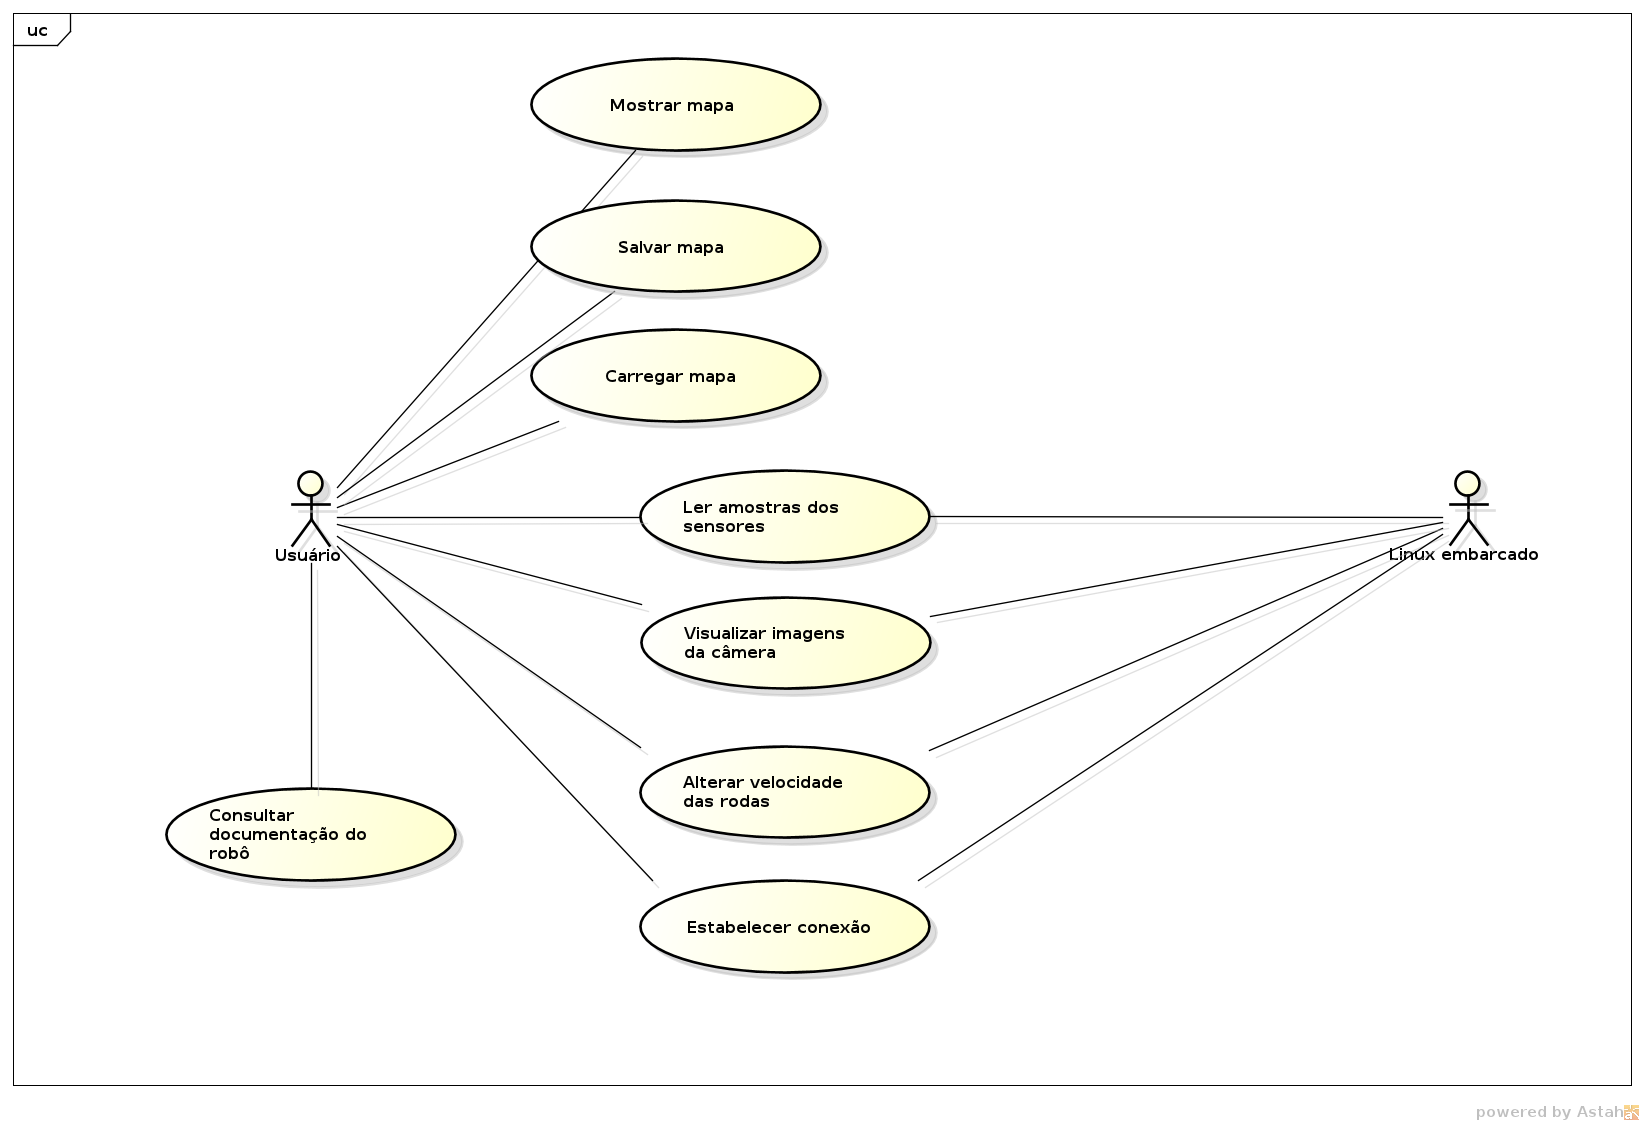
\includegraphics[width=\textwidth, keepaspectratio]{./figuras/diagrama_caso_uso_estacao_base.png}
  \caption{Diagrama de casos de uso do \textit{software} da estação base.}
  \label{fig:diagrama_caso_uso_estacao_base}
\end{figure}

\begin{figure}[H]
  \centering
  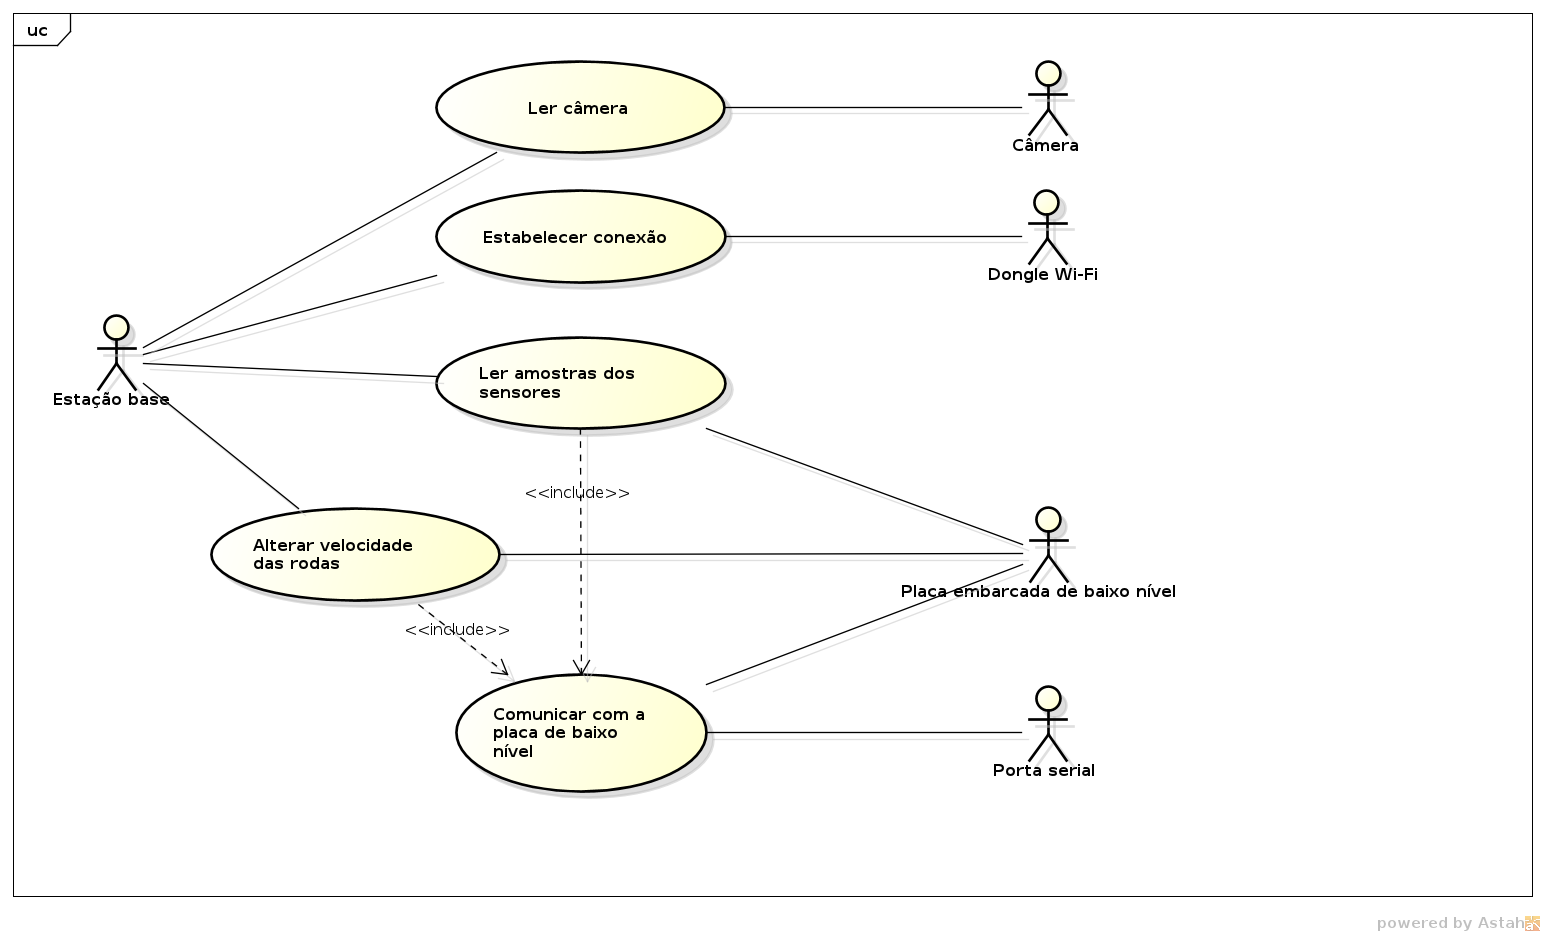
\includegraphics[width=\textwidth, keepaspectratio]{./figuras/diagrama_caso_uso_linux_embarcado.png}
  \caption{Diagrama de casos de uso do \textit{software} para a placa TS-7260.}
  \label{fig:diagrama_caso_uso_linux_embarcado}
\end{figure}

\begin{figure}[H]
  \centering
  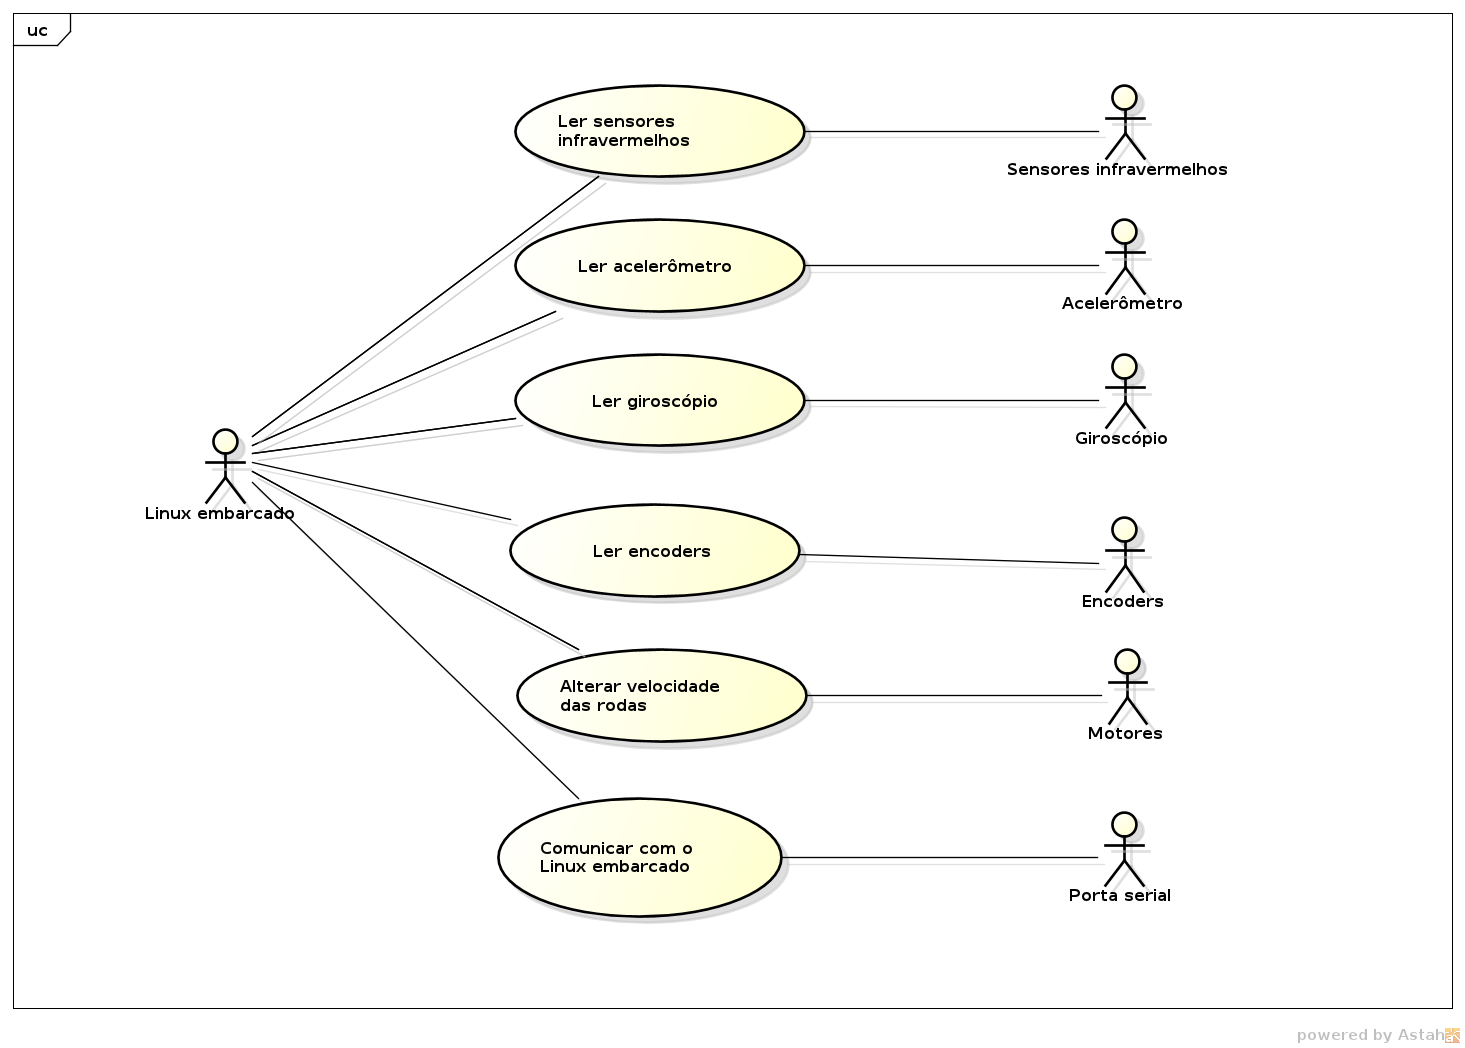
\includegraphics[width=\textwidth, keepaspectratio]{./figuras/diagrama_caso_uso_placa_embarcada.png}
  \caption{Diagrama de casos de uso do \textit{software} para a placa de baixo nível.}
  \label{fig:diagrama_caso_uso_placa_embarcada}
\end{figure}

\section{Diagrama de classes da estação base}

A Figura \ref{fig:diagrama_classes_estacao_base} mostra o diagrama de classes da estação base.
\begin{figure}[H]
  \centering
  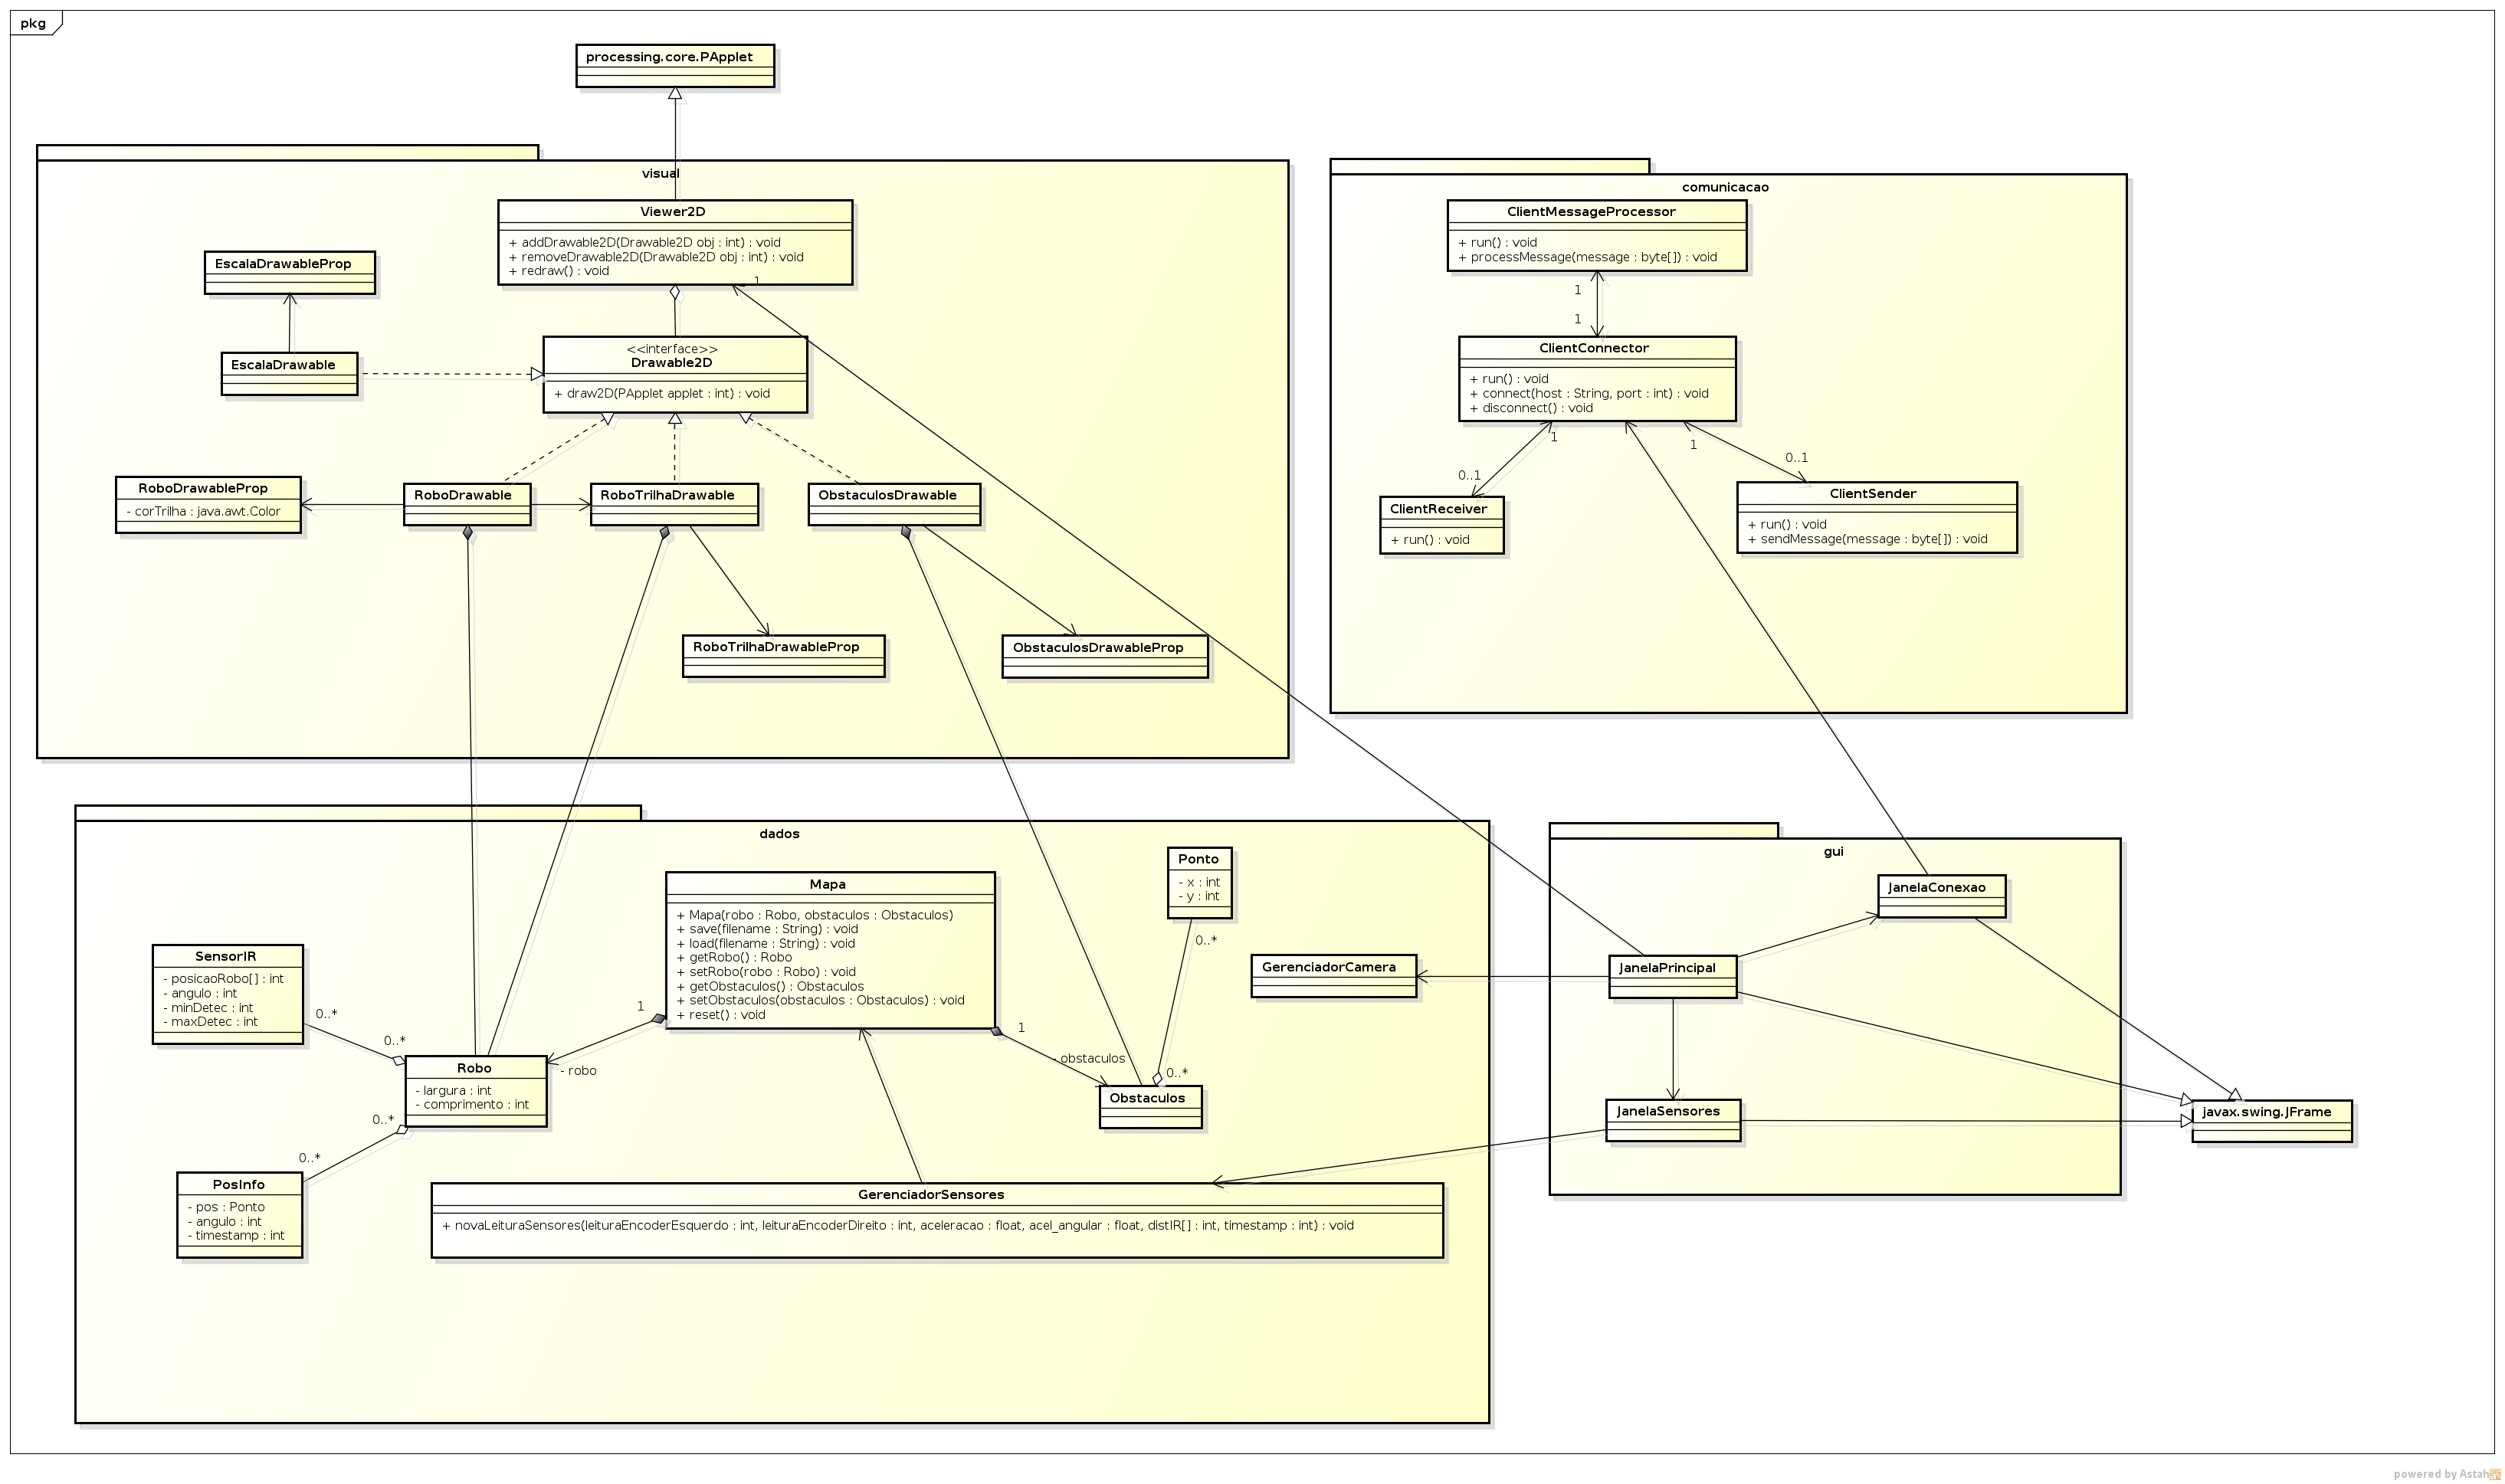
\includegraphics[width=\textwidth]{./figuras/diagrama_classes_estacao_base.png}
  \caption{Diagrama de classes da estação base}
  \label{fig:diagrama_classes_estacao_base}
\end{figure}

\subsection{Descrição das classes da estação base}
%O software da estação base do robô foi dividido em cinco pacotes:  visual, controle, comunicação, controle.robo e interface gráfica. Estes serão descritos com suas respectivas classes na Tabela \ref{tab:pacote_visual}.
O \textit{software} da estação base do robô foi dividido em cinco pacotes:  \textit{visual}, \textit{dados}, \textit{comunicao}, e \textit{gui}. A seguir há uma descrição de cada pacote e das suas respectivas classes.


\subsection{Pacote \textit{visual}}

Este pacote consiste de toda a parte visual da estação base e conta com as seguintes classes: Viewer2D, Drawable2D, EscalaDrawable, RoboDrawable, RoboTrilhaDrawable, ObstaculosDrawable, EscalaDrawableProp, RoboDrawableProp, RoboTrilhaDrawableProp e ObstaculosDrawableProp. Na Tabela \ref{tab:pacote_visual} estão descritas as classes deste pacote.


\begin{table}[h]
  \centering
  \caption{Pacote \textit{visual}}
  \begin{tabular}{p{6cm}p{8cm}}
    \toprule
    \textbf{Classe} & \textbf{Descrição} \\
    \midrule
    Viewer2D & Responsável por exibir os objetos Drawable2D. Possui recursos de pan, zoom e rotate.   \\ \hline
    Drawable2D & Representa genericamente objetos 2D que podem ser desenhados em um Viewer2D. \\ \hline
    EscalaDrawable & Responsável por desenhar uma escala gráfica no mapa. \\ \hline
    RoboDrawable & Responsável por desenhar o robô no mapa. \\ \hline
    RoboTrilhaDrawable & Responsável por desenhar a trilha percorrida pelo robô no mapa. \\ \hline
    ObstaculosDrawable & Responsável por desenhar os pontos de cada obstáculo no mapa. \\ \hline
    EscalaDrawableProp & Contém as propriedades visuais de desenho da escala. \\ \hline
    RoboDrawableProp & Contém as propriedades visuais de desenho do robô \\ \hline
    RoboTrilhaDrawableProp & Contém as propriedades visuais de desenho da trilha do robô. \\ \hline
    ObstaculosDrawableProp & Contém as propriedades visuais de desenho dos obstáculos. \\
    \bottomrule
  \end{tabular}%
  \label{tab:pacote_visual}%
\end{table}%

\subsection{Pacote \textit{dados}}

Este pacote consiste de toda a parte da estação base que processa e armazena as informações essenciais do robô e do mapa. Conta com as seguintes classes: Mapa, Obstaculos, Robo, ControleSensores, Posinfo, SensorIR e Ponto. Na Tabela \ref{tab:pacote_controle} estão descritas as classes deste pacote.

\begin{table}[h]
  \centering
  \caption{Pacote \textit{dados}}
  \begin{tabular}{p{6cm}p{8cm}}
    \toprule
    \textbf{Classe} & \textbf{Descrição} \\ 
    \midrule
    Mapa  & Responsável por representar o mapa. Armazena as informações essenciais do robô e dos obstáculos detectados. \\ \hline
    Obstaculos & Responsável por conter os obstáculos detectados pelo robô. \\ \hline
    Robo  & Responsável por representar o robô, este contêm largura, comprimento e centro de movimento (ponto central entre as duas rodas). \\ \hline
    GerenciadorSensores & Responsável por atualizar a posição do robô e dos pontos que representam os obstáculos, de acordo com as leituras feitas pelos sensores. \\ \hline
    Posinfo & Responsável por conter as informações de uma posição do robô. \\ \hline
    SensorIR & Responsável por representar um sensor IR do robô. \\ \hline 
    Ponto & Representa um ponto de cordenadas cartesianas (x,y). \\ \hline
    GerenciadorCamera & Responsável por gerenciar o status da câmera e o recebimento de imagens. \\ 
    \bottomrule
  \end{tabular}%
  \label{tab:pacote_controle}%
\end{table}%

\subsection{Pacote \textit{comunicacao}}
\label{subsec:pacote_comunicacao}

%Este pacote consiste em toda a parte de comunicação da estação base com o robô e conta com as seguintes classes: ClientCommandInterpreter, ClientConnection, ClientReceiver, ClientSender, ServerCommandInterpreter, ServerListener, ServerSender, ServerReceiver e Message. Na Tabela \ref{tab:pacote_comunicacao} estão descritas as classe deste pacote.
Este pacote consiste em toda a parte de comunicação da estação base com o robô e conta com as seguintes classes: ClientMessageProcessor ClientConnection, ClientReceiver, ClientSender e Message. Na Tabela \ref{tab:pacote_comunicacao} estão descritas as classes deste pacote.

É importante ressaltar que o protocolo TCP requer obrigatoriamente a especificação de um cliente e de um servidor para estabelecimento de uma conexão. Nas implementações desse protocolo em diversas linguagens (como Java e C++) existem tipos de \textit{socket} distintos para cliente e servidor. Na criação de um \textit{socket} de servidor, há obrigatoriamente a atribuição de uma porta de escuta, na qual o servidor aguarda que um cliente efetue uma requisição de conexão. Não é possível, ao menos nas implementações atuais do TCP, estabelecer conexão entre dois \textit{sockets} de cliente ou entre dois \textit{sockets} de servidor. Como neste projeto, o robô proverá serviços à estação base (envio de imagens da câmera, envio de leituras de sensores, além de prover a posibilidade de comando dos motores) o robô foi escolhido como servidor e a estação base como cliente. Enfatiza-se que o paradigma cliente-servidor não implica de forma alguma que a comunicação seja unidirecional. Pelo contrário, o envio de pacotes 
pode ser feito bidirecionalmente após uma conexão TCP ser estabelecida, sem nenhuma restrição quanto a isso.

\begin{table}[h]
  \centering
  \caption{Pacote \textit{comunicacao}}
  \begin{tabular}{p{6cm}p{8cm}}
    \toprule
    \textbf{Classe} & \textbf{Descrição} \\ 
    \midrule
    ClientMessageProcessor & Thread responsável pelo processamento de mensagens recebidas de um host de conexão. \\ \hline
    ClientConnector & Thread responsável por efetuar a gerência da conexão do cliente (estação base) com o servidor (robô). \\ \hline
    ClientReceiver & Thread responsável por receber mensagens de um host de uma conexão. \\ \hline
    ClientSender & Thread responsável por enviar mensagens ao host de uma conexão. \\ \hline
%    ServerCommandInterpreter & Responsável pela interpretação dos comandos do servidor. Os comandos recebidos são inseridos em uma fila, de modo a serem posteriormente executados pela thread. \\ \hline
%    Server & Responsável gerenciar o servidor (robô). \\ \hline
%    ServerListener & Responsável por escutar as novas conexões de clientes. \\ \hline
%    ServerSender & Responsável por enviar mensagens ao host de uma conexão. \\ \hline
%    ServerReceiver & Responsável por receber mensagens de um host de uma conexão. \\ \hline
%     Message & Contém uma mensagem a ser enviada por um Sender. \\ 
    \bottomrule
  \end{tabular}%
  \label{tab:pacote_comunicacao}%
\end{table}%

\subsection{Pacote \textit{gui}}

Este pacote consiste em toda a interface gráfica do sistema e conta com as seguintes classes: JanelaConexao, JanelaPrincipal e JanelaSensores. Na Tabela \ref{tab:pacote_interface_grafica} estão descritas as classes deste pacote.

\begin{table}[h]
  \centering
  \caption{Pacote \textit{gui}}
  \begin{tabular}{p{6cm}p{8cm}}
    \toprule
    \textbf{Classe} & \textbf{Descrição} \\ 
    \midrule
    JanelaConexao & Janela com as informações e configurações da conexão com o Bellator. \\ \hline
    JanelaPrincipal & Janela principal da interface gráfica da estação base. \\ \hline
    JanelaSensores & Janela de configuração dos sensores. \\ 
    \bottomrule
  \end{tabular}%
  \label{tab:pacote_interface_grafica}%
\end{table}%

\section{Fluxo de dados}

A Figura \ref{fig:diagrama_fluxo_dados} mostra o diagrama de fluxo de dados.

\begin{figure}[H]
  \centering
  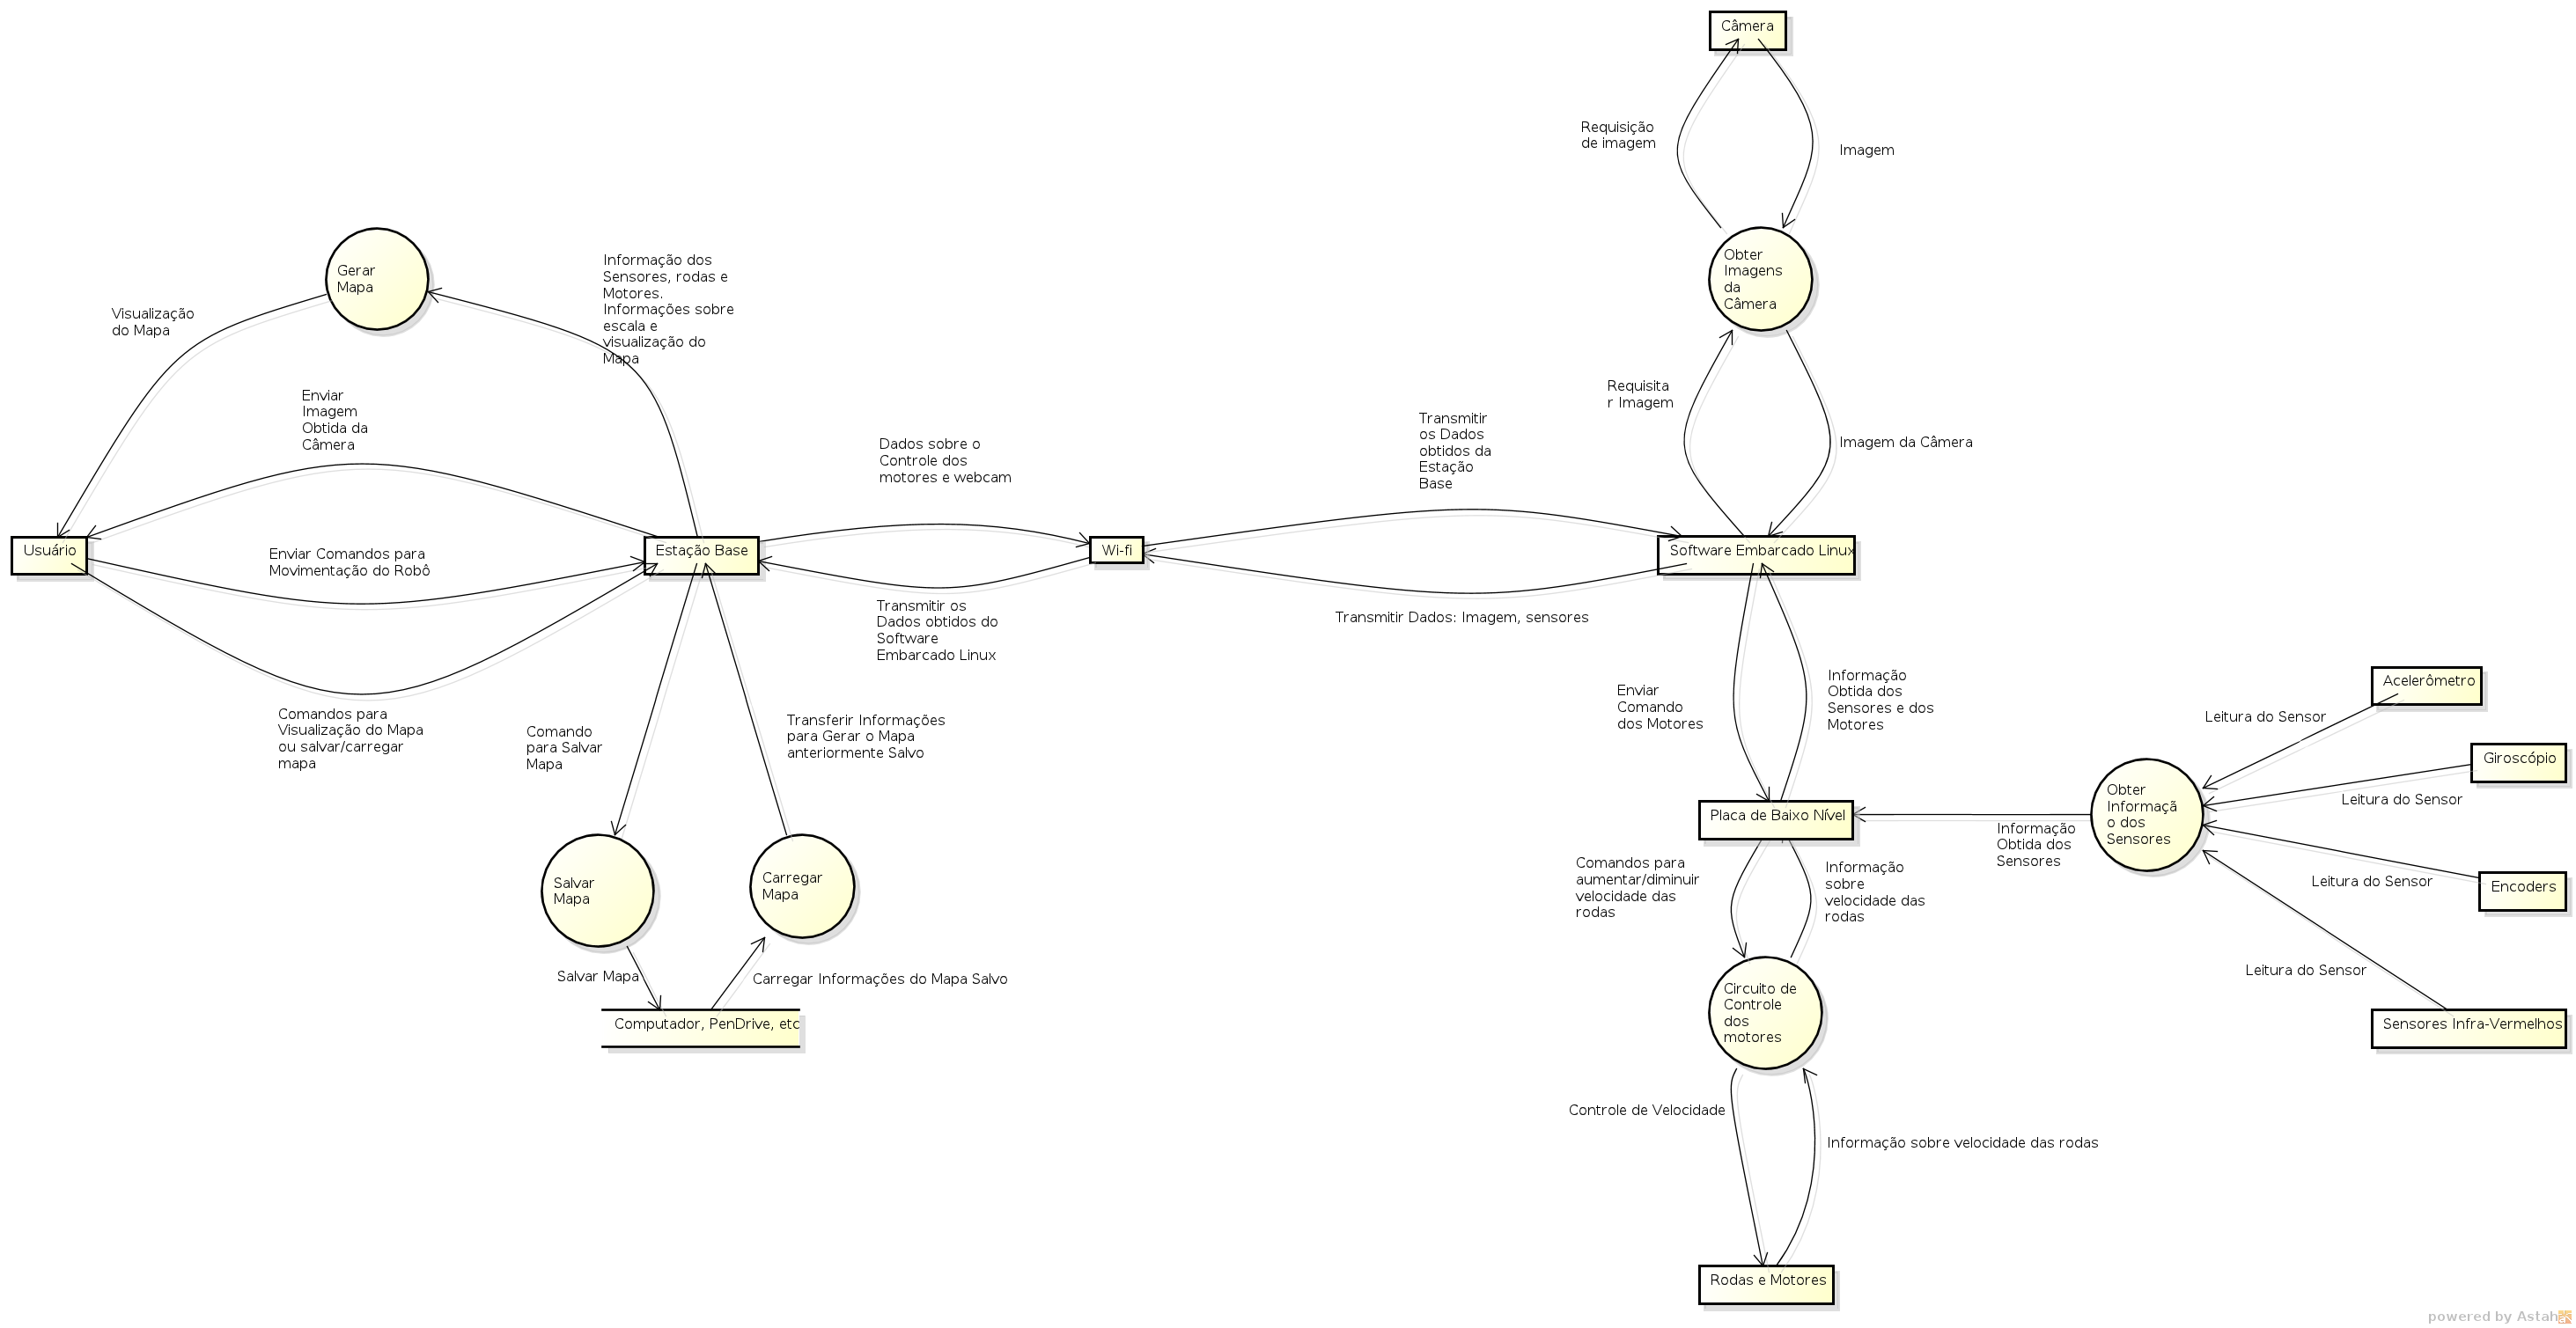
\includegraphics[width=\textwidth, keepaspectratio]{./figuras/diagrama_fluxo_dados.png}
  \caption{Diagrama de fluxo de dados.}
  \label{fig:diagrama_fluxo_dados}
\end{figure}

% \section{Diagrama de estados}
% As Figuras \ref{fig:diagrama_estados_estacao_base} e \label{fig:diagrama_estados_sistema_embarcado} mostram os diagramas de estados do sistema.
% 
% \begin{figure}[H]
%   \centering
%   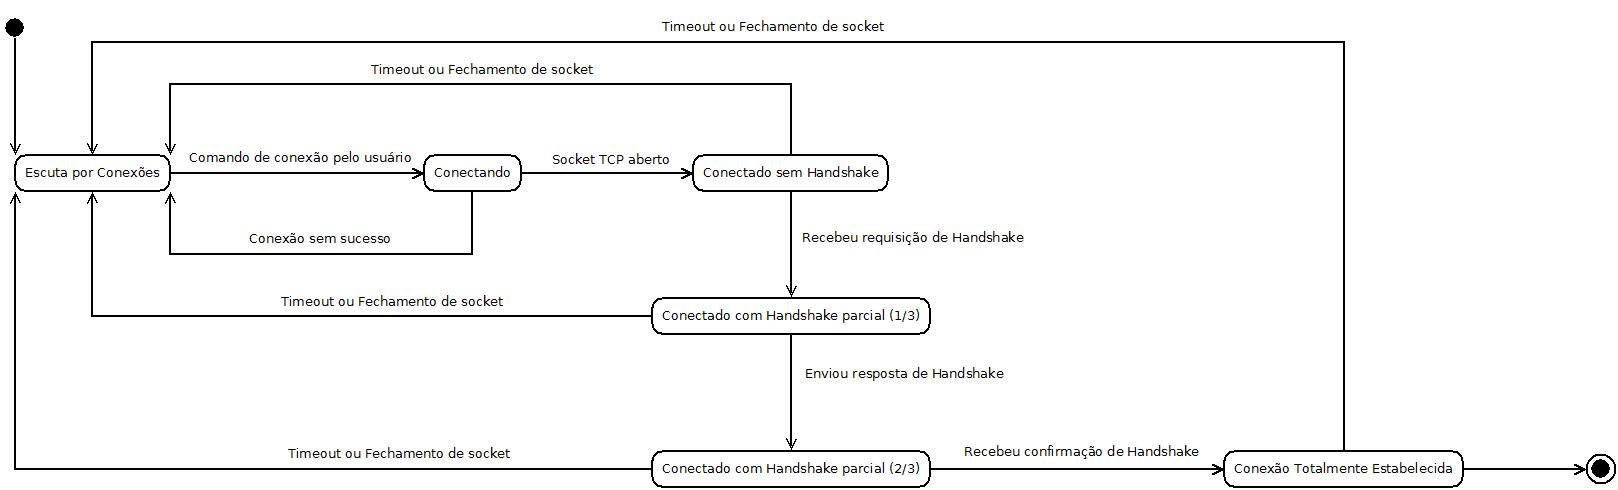
\includegraphics[width=\textwidth, keepaspectratio]{./figuras/diagrama_estados_estacao_base.jpeg}
%   \caption{Diagrama de estados para a estação base.}
%   \label{fig:diagrama_estados_estacao_base}
% \end{figure}
% 
% \begin{figure}[H]
%   \centering
%   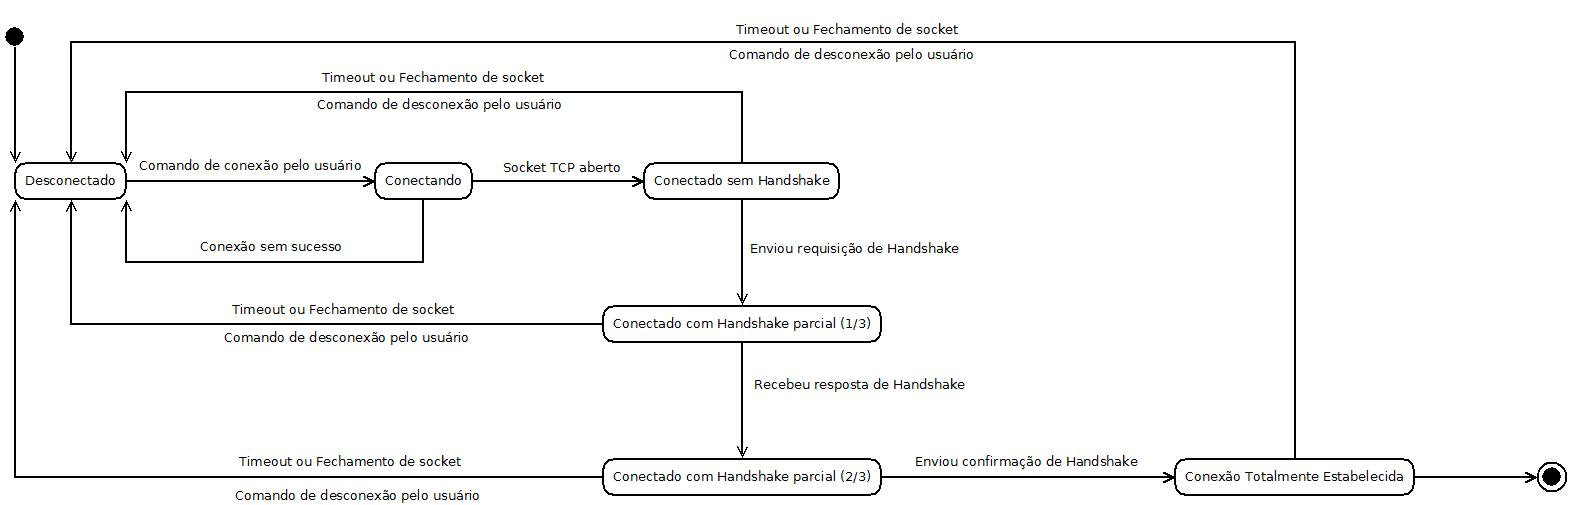
\includegraphics[width=\textwidth, keepaspectratio]{./figuras/diagrama_estados_sistema_embarcado.jpeg}
%   \caption{Diagrama de estados para o sistema embarcado.}
%   \label{fig:diagrama_estados_sistema_embarcado}
% \end{figure}


\section{Diagrama de classes do sistema embarcado}


A Figura \ref{fig:diagrama_classes_sist_embarcado} mostra o diagrama de classes do sistema embarcado (placa TS-7260).
\begin{figure}[H]
  \centering
  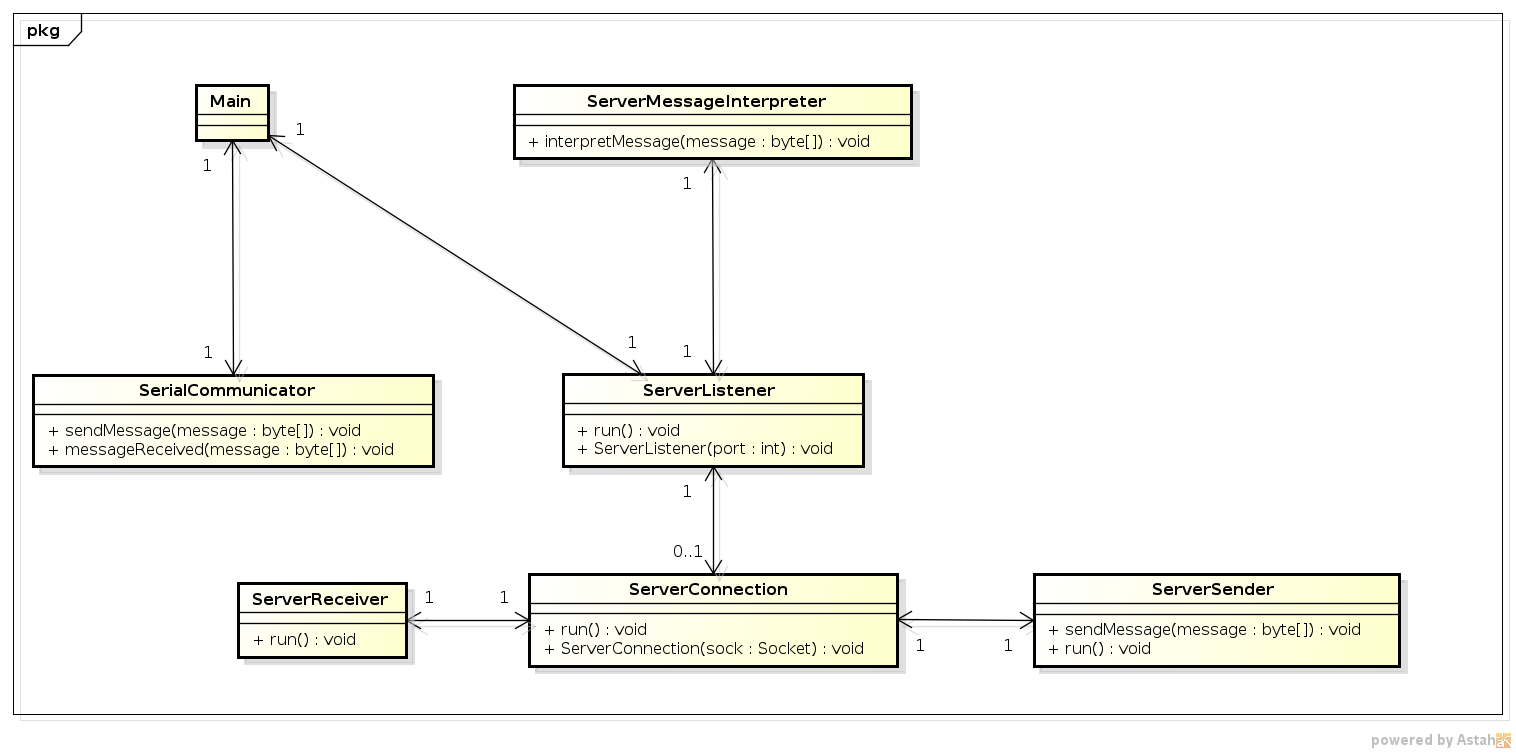
\includegraphics[width=\textwidth]{./figuras/diagrama_classes_sist_embarcado.png}
  \caption{Diagrama de classes do sistema embarcado (placa TS-7260).}
  \label{fig:diagrama_classes_sist_embarcado}
\end{figure}



%\subsection{Descrição das classes do sistema embarcado (TS-7260)}

\begin{table}[h]
  \centering
  \caption{Descrição das classes do sistema embarcado (placa TS-7260)}
  \begin{tabular}{p{6cm}p{8cm}}
    \toprule
    \textbf{Classe} & \textbf{Descrição} \\ 
    \midrule
   Main & Classe principal do robô. \\ \hline
   SensorsSampler & Thread responsável por requisitar amostras dos sensores da plca de baixo nível em intervalos de tempo previamente programados. \\ \hline
   ServerMessageProcessor & Thread responsável por realizar o processamento de mensagens recebidas de um host de conexão. \\ \hline
   ServerListener & Thread responsável por escutar requisições de conexão. \\ \hline
   ServerSender & Thread responsável por enviar mensagens ao host de uma conexão. \\ \hline
   ServerReceiver & Thread responsável por receber mensagens de um host de uma conexão. \\ \hline
   SerialCommunicator & Responsável por gerenciar a comunicação via porta serial entre a TS-7260 e a LPC2103.\\
    \bottomrule
  \end{tabular}%
  \label{tab:pacote_comunicacao}%
\end{table}%



\section{Protocolo de comunicação}

Esta seção detalha o protocolo de comunicação estabelecido entre a estação base, a placa TS-7260 (sistema com linux embarcado) e a placa LPC2103 (sistema embarcado de baixo nível).

O protocolo desenvolvido para a comunicação (via Wi-Fi) entre a estação base e a TS-7260 visa utilizar o TCP como camada de transporte. Como foi explicitado anteriormente na seção \ref{subsec:pacote_comunicacao}, o robô foi escolhido como servidor da conexão, e a estação base como cliente. Para haver confirmação da conexão entre os dois, optou-se por criar um protocolo de \textit{handshake} semelhante ao existente no TCP, de 3 passos: requisição, resposta, confirmação. A requisição é feita pelo cliente no início da conexão, a resposta é dada pelo servidor em seguida. Posteriormente, o cliente envia uma mensagem de confirmação, e a conexão é totalmente estabelecida. O uso do \textit{handshake} contribui para tanto a estação base como o sistema embarcado confirmarem que estão conectados um ao outro e não a um servidor/cliente qualquer.

Para possibilitar que o tráfego de mensagens possa ser feito de forma rápida, reduzindo atrasos, o envio e recebimento de mensagens é feito de forma assíncrona.
Essa escolha foi feita tendo em vista que, em uma comunicação totalmente síncrona, um programa (ou thread) é bloqueado ao chamar uma função de recebimento ou envio, até que efetivamente seja completa a transação. Supondo que só houvesse uma thread gerenciando a conexão, o programa não poderia enviar ou receber dados ao mesmo tempo em \textit{full-duplex}, mas somente \textit{half-duplex} (somente enviar ou somente receber).

A solução desenvolvida para possibilitar a comunicação assíncrona foi o uso de 4 threads (tanto na estação base quanto no sistema embarcado) para gerenciar os diversos aspectos envolvidos nela. A primeira \textit{thread} (a gerenciadora principal de conexão) é a responsável por estabelecer e manter a conexão, além de gerenciar os potenciais erros que possam ocorrer (tempo excessivo sem comunicação e fechamento de socket). Para a estação base, o diagrama de estados dessa \textit{thread} está representado na Figura \ref{fig:diagrama_estados_estacao_base}, e para o sistema embarcado na Figura \ref{fig:diagrama_estados_sist_embarcado}.

A segunda \textit{thread} tem a função de gerenciar o envio de mensagens. O programa principal, ao necessitar enviar uma mensagem, faz uma requisição a essa \textit{thread} que insere a mensagem em uma fila de envio. O programa principal não fica bloqueado, dessa forma, pois não necessita aguardar a mensagem ser completamente enviada, podendo efetuar outras tarefas. O diagrama de estados dessa \textit{thread} está presente na Figura \ref{fig:diagrama_estados_sender}.

A terceira \textit{thread} gerencia o recebimento de mensagens. Seu funcionamento é relativamente simples: ela possui um loop, no qual aguarda até alguma mensagem ser recebida. Quando ocorre o recebimento de alguma mensagem, ela é encaminhada para a quarta \textit{thread} (cuja explicação está a seguir) que processa o conteúdo dela e executa as operações que são necessárias para cada tipo de mensagem. Dessa forma, novas mensagens podem ser recebidas rapidamente, pois o receptor não fica bloqueado realizando o processamento das informações recebidas. O diagrama de estados dessa terceira \textit{thread} está presente na Figura \ref{fig:diagrama_estados_receiver}.

A quarta \textit{thread}, como já exposto, é a responsável por processar mensagens recebidas e realizar as operações que são necessárias para cada tipo de mensagem, o que depende da codificação exposta na seção \ref{sec:codificacao_mensagens}. Ela possui uma fila, na qual são inseridas as mensagens a serem processadas. Dessa forma a \textit{thread} receptora não necessita ficar bloqueada aguardando o término do processamento. O diagrama de estados dessa quarta \textit{thread} está presente na Figura \ref{fig:diagrama_estados_processor}.


\subsection{Codificação das mensagens}
\label{sec:codificacao_mensagens}

\begin{itemize}
  \item Mensagens do TS-7260 para o LPC2103 (via porta serial)
    	
	\begin{itemize}
		
	  \item \textbf{SYNC (0xA0)}\\
	  Quando o microcontrolador LPC2103 recebe esta mensagem, responde com as leituras mais recentes dos encoders, de cada sensor de distância, do acelerômetro e do giroscópio (enviando uma mensagem SENSORS, explicada abaixo).
	  
	  \item \textbf{ENGINES (0xB0)}\\
	  \textit{(byte) vel\_roda\_esquerda}\\
	  \textit{(byte) vel\_roda\_direita}\\
	  \textit{(byte) CHECKSUM\_H}\\
	  \textit{(byte) CHECKSUM\_L}\\
	  Ao receber este comando, o microcontrolador utiliza os valores para definir o nível de PWM para as rodas do robô. Os valores de velocidade são representados por um byte cada, nos quais o bit mais significativo indica o sentido de rotação da roda (1 para frente e 0 para trás) e os restantes a intensidade do PWM.
	  
	  Os bytes de checksum são utilizados para verificar se não há dados corrompidos. Os bytes da mensagem são somados (módulo 65536) e o resultado é atribuído aos bytes (high e low) de checksum.
	  \end{itemize}
	  
	  \item Mensagens do LPC2103 para a TS-7260 (via porta serial)
	  
	  \begin{itemize}

	  \item \textbf{ENGINES\_ACK (0xB1)}\\
	  \textit{(byte) vel\_roda\_esquerda}\\
	  \textit{(byte) vel\_roda\_direita}\\
	  \textit{(byte) CHECKSUM\_H}\\
	  \textit{(byte) CHECKSUM\_L}\\
	  Esta mensagem deve ser enviada toda vez que um comando de mudança de velocidade (ENGINES) for recebido na placa de baixo nível. A mensagem é usada no Linux embarcado para verificar se o comando foi corretamente recebido. Caso uma confirmação não seja recebida em certo intervalo de tempo, outro comando ENGINES é enviado para a placa de baixo nível.
	 
	  O checksum é tem função idêntica ao que já foi explicitado na mensagem ENGINES.
	  
	  \item \textbf{SENSORS (0xC0)}\\
	  \textit{(byte) encoder\_esq\_H}, \textit{(byte) encoder\_esq\_L},\\
	  \textit{(byte) encoder\_dir\_H}, \textit{(byte) encoder\_dir\_L},\\
	  \textit{(byte) IR1}, \textit{(byte) IR2}, \textit{(byte) IR3}, \textit{(byte) IR4}, \textit{(byte) IR5},\\
	  \textit{(byte) AX\_H}, \textit{(byte) AX\_L},\\
	  \textit{(byte) AY\_H}, \textit{(byte) AY\_L},\\
	  \textit{(byte) AZ\_H}, \textit{(byte) AZ\_L},\\
	  \textit{(byte) GX\_H}, \textit{(byte) GX\_L},\\
	  \textit{(byte) GY\_H}, \textit{(byte) GY\_L},\\
	  \textit{(byte) GZ\_H}, \textit{(byte) GZ\_L},\\
	  \textit{(byte) TIMESTAMP\_H}, \textit{(byte) TIMESTAMP\_L}\\
	  \textit{(byte) CHECKSUM\_H}\\
	  \textit{(byte) CHECKSUM\_L}\\
	  Representa a leitura de todos os sensores (encoders, infra-vermelhos, acelerômetro e giroscópio). 
	  
	  Os 4 primeiros bytes são os valores das leituras dos encoders esquerdo e direíto (cada um com um byte alto e um baixo). Os valores das leituras dos encoders representam a diferença entre a contagem atual a contagem anterior.
	  
	  Nos próximos 5 bytes, as leituras do sensores ópticos são enviadas em sequência. As distâncias que os sensores ópticos são capazes de mensurar são dividos em valores discretos de 0 a 255 \cite{bellator_2012}. 
	  
	  Após isso, os 12 bytes que se seguem representam as leituras do acelerômetro e do giroscópio. Os bytes que começam com `A' representam a leitura de cada um dos eixos do acelerômetro. Aqueles que começam com `G' representam a leitura de cada um dos eixos do giroscópio.
	  
	  O timestamp (valor alto e baixo) é um contador de 16 bits que é incrementado entre cada amostra e zera automaticamente depois que chega ao valor máximo (65535), usado para determinar o instante em que foi feita a leitura dos dados. Como a amostragem dos sensores na placa de baixo nível será efetuada em intervalos fixos, a informação do contador do timestamp pode ser utilizada para obter informações de tempo de cada amostra.

	  O checksum é tem função idêntica ao que já foi explicitado na mensagem ENGINES.
	  
	  
	\end{itemize}

  \item Mensagens bidirecionais entre estação base e TS-7260 (via Wi-Fi):

    \begin{itemize}
      \item \textbf{ECHO\_REQUEST (0x01)}\\
      \textit{(byte) END\_CMD}\\
	Requisição de ping.
      \item \textbf{ECHO\_REPLY (0x02)}\\
      \textit{(byte) END\_CMD}\\
	Resposta de ping.
      \item \textbf{DISCONNECT (0x0F)} \\
	Solicitação de desconexão.
    \end{itemize}

  \item Mensagens da estação base para a TS-7260 (via Wi-Fi):

    \begin{itemize}
      \item \textbf{HANDSHAKE\_REQUEST (0x10)}\\
	Solicitação de handshake.

      \item \textbf{HANDSHAKE\_CONFIRMATION (0x12)}\\
	Confirmação de handshake.

      \item \textbf{SENSORS\_START (0x20)}\\
	Solicitação de início da amostragem dos sensores.

      \item \textbf{SENSORS\_STOP (0x21)}\\
	Solicitação de parada da amostragem dos sensores.

      \item \textbf{SENSORS\_RATE (0x22)} \\
	\textit{(float) Nova taxa de amostragem (comandos SYNC por segundo)}\\
	Solicitação de mudança da taxa de envio de comandos SYNC da TS para a placa de baixo nível.

%       \item \textbf{SENSORS\_STATUS\_REQUEST}\\
%       \textit{(byte) END\_CMD}\\
% 	Requisição de status da amostragem dos sensores. Usado na interface gráfica para atualizar as informações sobre os sensores.

      \item \textbf{WEBCAM\_START (0x30)}\\
	Solicitação de início da amostragem da webcam.

      \item \textbf{WEBCAM\_STOP (0x31)}\\
	Solicitação de parada da amostragem da webcam.

      \item \textbf{WEBCAM\_RATE (0x32)} \\
	\textit{(float) Nova taxa de quadros}\\
	Solicitação de mudança da taxa de quadros da webcam.

      \item \textbf{WEBCAM\_RESOLUTION (0x33)} \\
	\textit{(int) Largura em pixels }\\
	\textit{(int) Altura em pixels}\\
	Solicitação de mudança da resolução da webcam.

%       \item \textbf{WEBCAM\_STATUS\_REQUEST}\\
%       \textit{(byte) END\_CMD}\\
% 	Solicitação de informações sobre status da webcam. Usado na interface gráfica para atualizar as informações sobre a webcam.

      \item \textbf{ENGINES (0xB0)} \\
	 \textit{(float) vel\_roda\_esquerda}\\
	 \textit{(float) vel\_roda\_direita}\\
	Solicitação de mudança da velocidade dos motores. Para cada roda há um valor de -1 até 1, sendo que -1 é a máxima velocidade para trás, 1 a máxima velocidade para frente e 0 é parada da roda.

%       \item \textbf{ENGINES\_STATUS\_REQUEST}\\
%       \textit{(byte) END\_CMD}\\
% 	Solicitação de status dos motores. Usado na interface gráfica para confirmar o recebimento de comandos de movimentação efetuados pelo usuário.

    \end{itemize}

  \item Mensagens da TS-7260 para a estação base (via Wi-Fi):

    \begin{itemize}
      \item \textbf{HANDSHAKE\_REPLY (0x11)}\\
	Resposta de handshake.
	
	 \item \textbf{SENSORS (0xC0)}\\
	  \textit{(byte) encoder1\_H}, \textit{(byte) encoder1\_L},\\
	  \textit{(byte) encoder2\_H}, \textit{(byte) encoder2\_L},\\
	  \textit{(byte) IR1}, \textit{(byte) IR2}, \textit{(byte) IR3}, \textit{(byte) IR4}, \textit{(byte) IR5},\\
	  \textit{(byte) AX\_H}, \textit{(byte) AX\_L},\\
	  \textit{(byte) AY\_H}, \textit{(byte) AY\_L},\\
	  \textit{(byte) AZ\_H}, \textit{(byte) AZ\_L},\\
	  \textit{(byte) GX\_H}, \textit{(byte) GX\_L},\\
	  \textit{(byte) GY\_H}, \textit{(byte) GY\_L},\\
	  \textit{(byte) GZ\_H}, \textit{(byte) GZ\_L},\\
	  \textit{(byte) TIMESTAMP\_H}, \textit{(byte) TIMESTAMP\_L}\\
	  
	  Possui a mesma funcionalidade e parâmetros que a mensagem SENSORS enviada da LPC2103 para a TS-7260, com exceção do timestamp, que é trocado por um timestamp UNIX em milissegundos (que representa o horário absoluto em que a amostra foi obtida na placa de baixo nível). Essa informação de tempo é utilizada pela estação base para efetuar os cálculos de posicionamento do robô.

      \item \textbf{SENSORS\_STATUS (0xC1)} \\
	\textit{(boolean) Status da amostragem [on - off] }\\
	\textit{(float) Taxa de amostragem}\\
	Informações de status dos sensores. Usado na interface gráfica para confirmar o recebimento de comandos de mudança de taxa de amostragem e início/parada da amostragem.

      \item \textbf{WEBCAM\_STATUS (0x34)} \\
% 	\textit{(boolean) Nova taxa de amostragem }\\
	\textit{(float) Taxa de quadros }\\
	\textit{(int) Largura em pixels }\\
	\textit{(int) Altura em pixels }\\
	\textit{(boolean) Status da stream [on - off] }\\
	\textit{(int) Porta da stream}\\
	Informações de status da webcam. Usado na interface gráfica para confirmar o recebimento de comandos relativos à webcam, e para que a estação base tenha conhecimento do status da stream da webcam.
	
      \item \textbf{ENGINES\_STATUS (0xB1)} \\
	\textit{(byte) vel\_roda\_esquerda}\\
	\textit{(byte) vel\_roda\_direita}\\
	Informações sobre as velocidades programadas dos motores. Usado na interface gráfica para confirmar o recebimento de comandos de movimentação efetuados pelo usuário.

	

    \end{itemize}
\end{itemize}


\subsection{Diagramas de estados}

Nesta seção estão expostos os diagramas de estados do protocolo de comunicação.

% nas Figuras \ref{fig:diagrama_estados_estacao_base}, \ref{fig:diagrama_estados_sist_embarcado}, \ref{fig:diagrama_estados_sender}, \ref{fig:diagrama_estados_receiver}, \ref{fig:diagrama_estados_processor} e \ref{fig:diagrama_estados_amostragem_sensores}.

Um aspecto importante a ressaltar é que, nas \textit{threads} de envio (Figura \ref{fig:diagrama_estados_sender}) e de processamento de mensagens (Figura \ref{fig:diagrama_estados_processor}), pode haver adição assíncrona de elementos na fila. Ou seja, quando é feita a verificação do número de elementos presentes na fila (como representado nos diagramas), tem-se em vista que elementos podem ter sido adicionados a qualquer instante. Obviamente, no ponto de vista da implementação, existem as seções críticas que devem ser devidamente gerenciadas para evitar condições de disputa e outros problemas de concorrência. Porém, as seções críticas se resumem aos acessos à fila somente, o que reduz consideravelmente a complexidade do processo.

Na Figura \ref{fig:diagrama_estados_motores_sist_embarcado} está explicitado o diagrama de estados da \textit{thread} responsável por gerenciar o envio de comandos de velocidade de motores (ENGINES) para a placa de baixo nível. Ela inicialmente aguarda que um comando ENGINES chegue da estação base, e quando isso ocorre, é enviado via serial o comando para a placa de baixo nível. A \textit{thread} aguarda certo tempo para receber um ENGINES\_ACK da placa de baixo nível para confirmar que o comando foi corretamente recebido. Caso isso não ocorra dentro do tempo estabelecido (por exemplo, se houver perda de pacotes), outro comando ENGINES é enviado. Isso ocorre até que um ENGINES\_ACK correto seja recebido da placa de baixo nível.

Na Figura \ref{fig:diagrama_estados_amostragem_sensores_sist_embarcado} está exposto o diagrama de estados da \textit{thread} do Linux embarcado que é responsável por realizar a amostragem dos sensores em intervalos fixos de tempo. Ela realiza a amostragem enviando periodicamente -- quando programada -- comandos SYNC (vide seção \ref{sec:codificacao_mensagens}) para a placa de baixo nível. Vale ressaltar que para melhor explicar este processo, na Figuras \ref{fig:diagrama_sequencia_sensores_sist_embarcado} e \ref{fig:diagrama_sequencia_sensores_estacao_base} da próxima seção está exposto um diagrama de sequência que demonstra a amostragem dos sensores.

Nas Figuras \ref{fig:diagrama_estados_webcam_estacao_base} e \ref{fig:diagrama_estados_webcam_sist_embarcado} estão presentes os diagramas de estados da captura e recebimento de imagens da webcam. Foi utilizada a biblioteca externa \textit{libVLC} \cite{vlc} -- a componente de baixo nível do \textit{player} de mídia VLC -- tanto na estação base como no Linux embarcado para efetuar o processo de transmissão e visualização de imagens. No Linux embarcado, quando um comando de início de webcam é dado pelo usuário, uma \textit{stream} HTTP de imagens é aberta pela \textit{libVLC}, e a estação base é posteriormente notificada sobre o fato. Na estação base, quando ocorre a notificação de que a stream foi aberta, a componente de \textit{player} da \textit{libVLC} da janela principal é ativada (conectando dessa forma, na stream HTTP de imagens).



\begin{figure}[H]
  \centering
  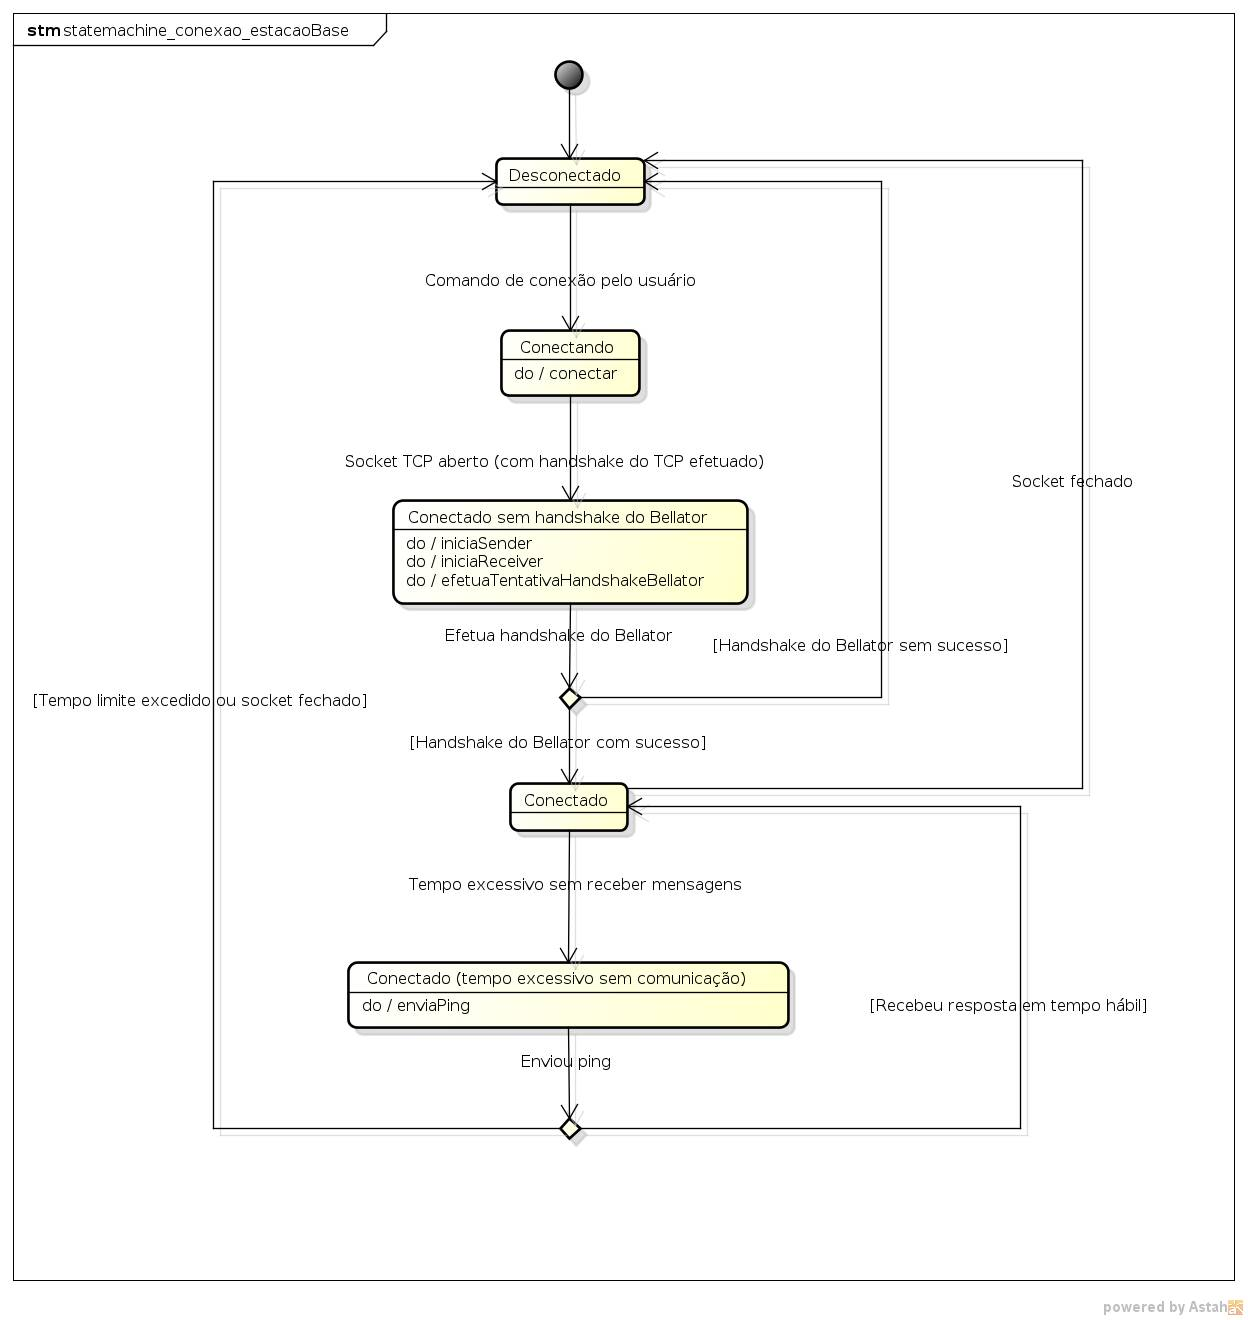
\includegraphics[width=\textwidth, keepaspectratio]{./figuras/estacaoBase/statemachine_conexao_estacaoBase.jpg}
  \caption{Diagrama estados da \textit{thread} principal da conexão da estação base.}
  \label{fig:diagrama_estados_estacao_base}
\end{figure}

\begin{figure}[H]
  \centering
  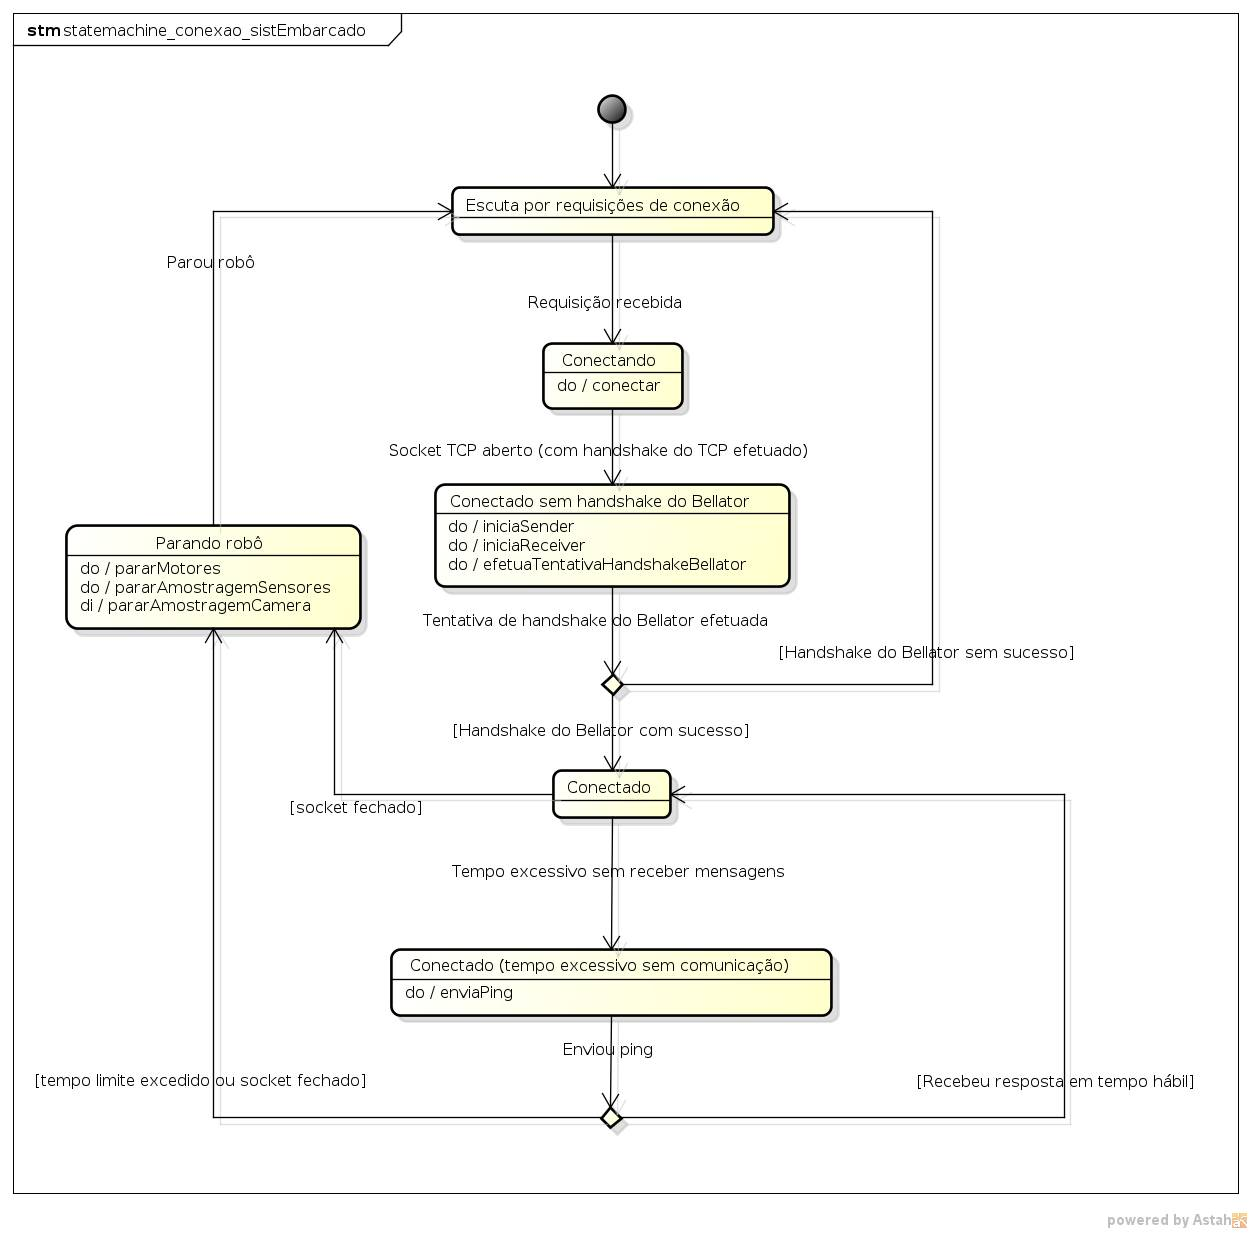
\includegraphics[width=\textwidth, keepaspectratio]{./figuras/sistEmbarcado/statemachine_conexao_sistEmbarcado.jpg}
  \caption{Diagrama de estados da \textit{thread} principal da conexão do linux embarcado.}
  \label{fig:diagrama_estados_sist_embarcado}
\end{figure}

\begin{figure}[H]
  \centering
  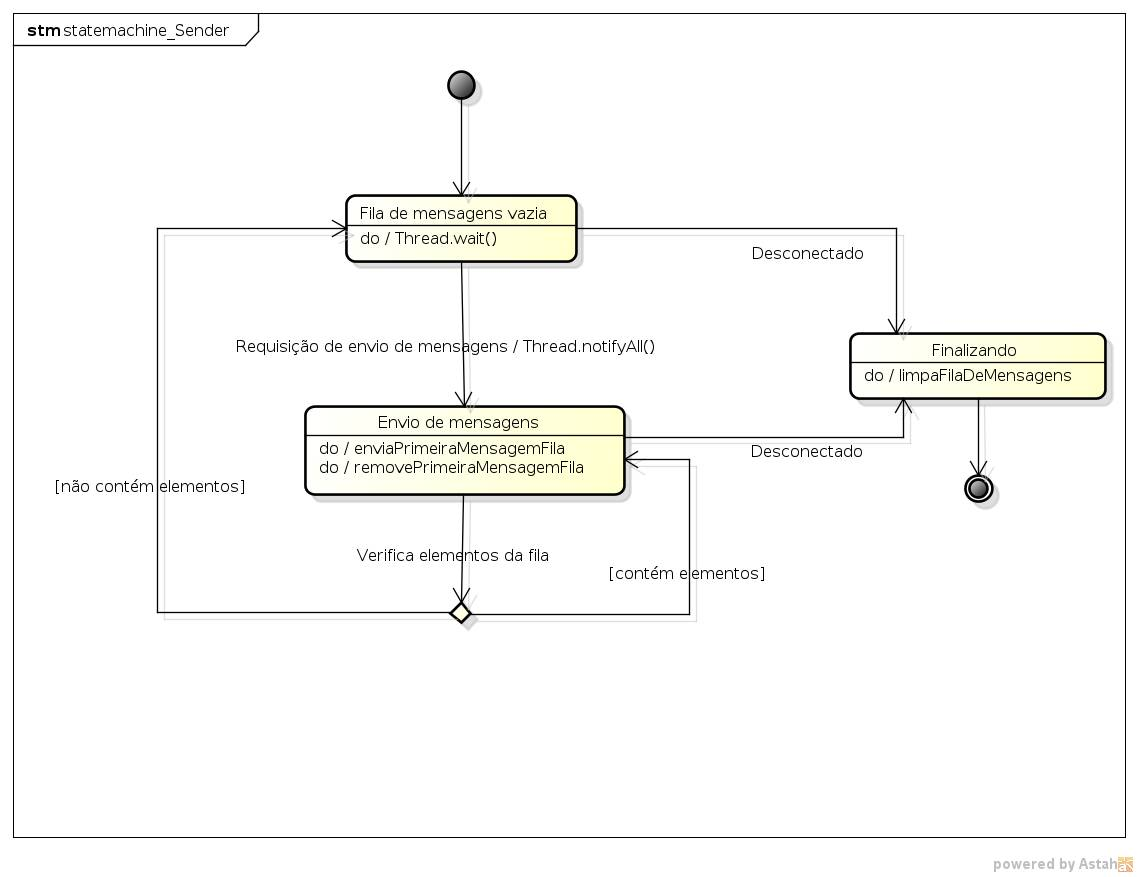
\includegraphics[width=\textwidth, keepaspectratio]{./figuras/statemachine_Sender.jpg}
  \caption{Diagrama de estados da \textit{thread} que envia mensagens (igual para estação base e linux embarcado).}
  \label{fig:diagrama_estados_sender}
\end{figure}

\begin{figure}[H]
  \centering
  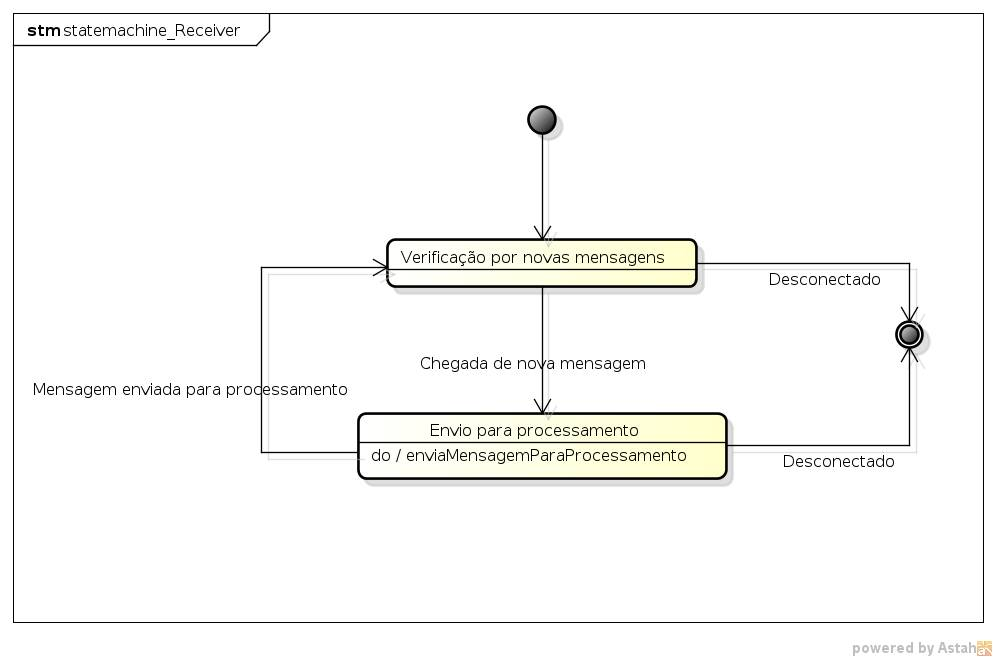
\includegraphics[width=\textwidth, keepaspectratio]{./figuras/statemachine_Receiver.jpg}
  \caption{Diagrama de estados da \textit{thread} receptora de mensagens (igual para estação base e linux embarcado).}
  \label{fig:diagrama_estados_receiver}
\end{figure}

\begin{figure}[H]
  \centering
  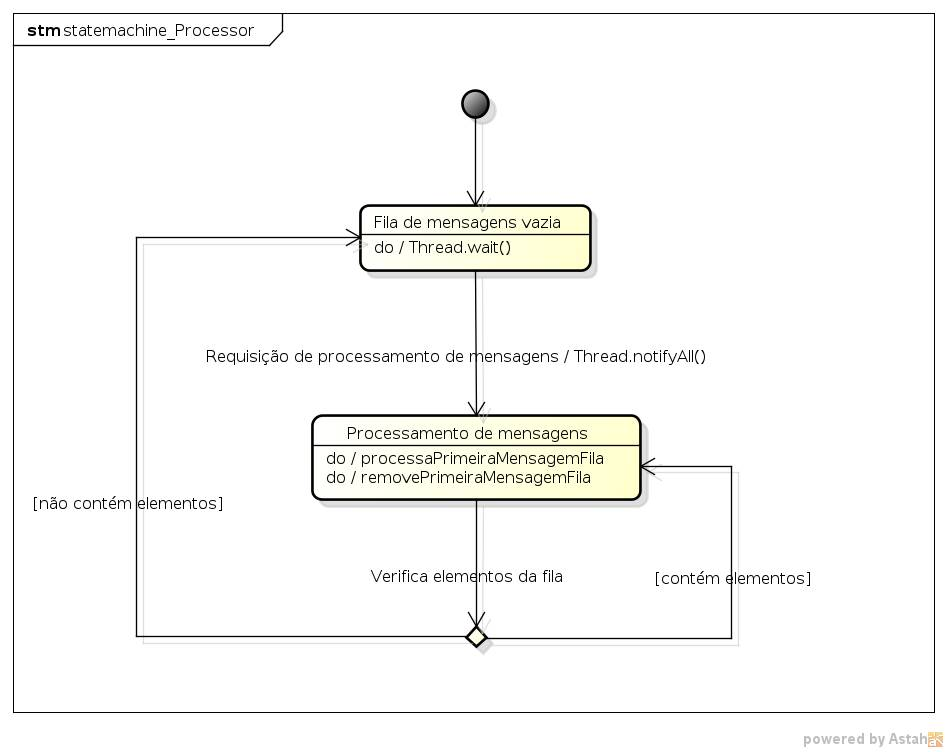
\includegraphics[width=\textwidth, keepaspectratio]{./figuras/statemachine_Processor.jpg}
  \caption{Diagrama de estados da \textit{thread} que processa mensagens recebidas (igual para estação base e linux embarcado).}
  \label{fig:diagrama_estados_processor}
\end{figure}

\begin{figure}[H]
  \centering
  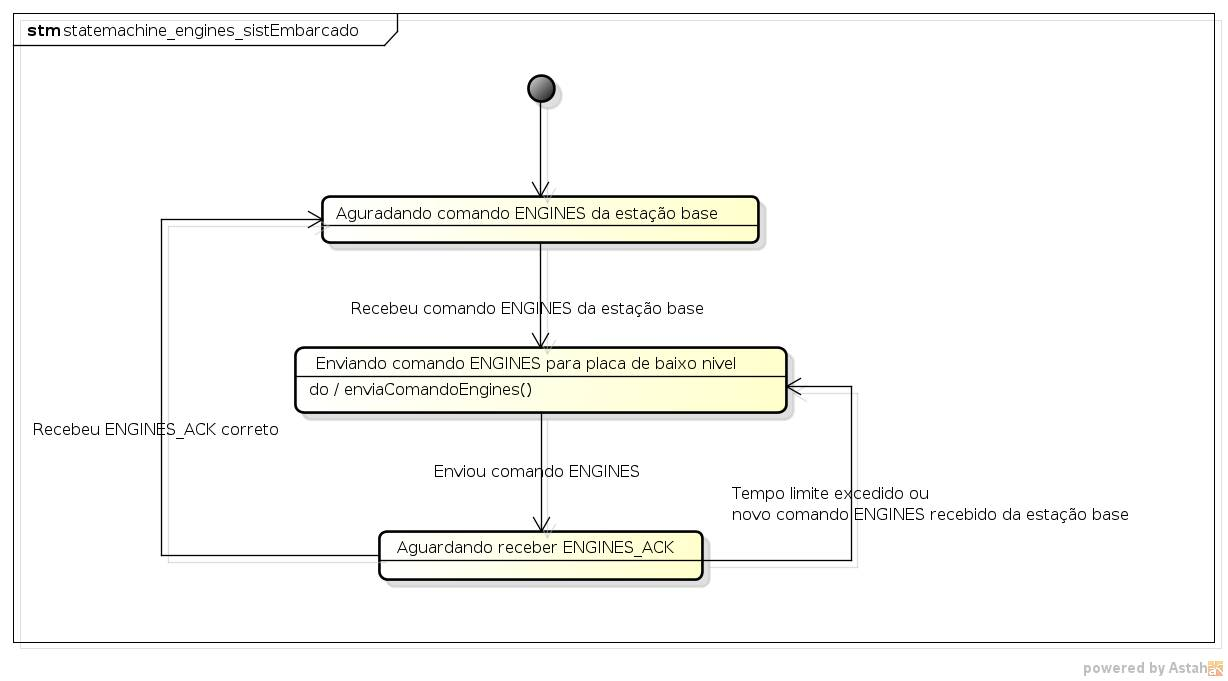
\includegraphics[width=\textwidth, keepaspectratio]{./figuras/sistEmbarcado/statemachine_motores_sistEmbarcado.jpg}
  \caption{Diagrama de estados da \textit{thread} responsável por gerenciar os comandos dos motores (linux embarcado).}
  \label{fig:diagrama_estados_motores_sist_embarcado}
\end{figure}

\begin{figure}[H]
  \centering
  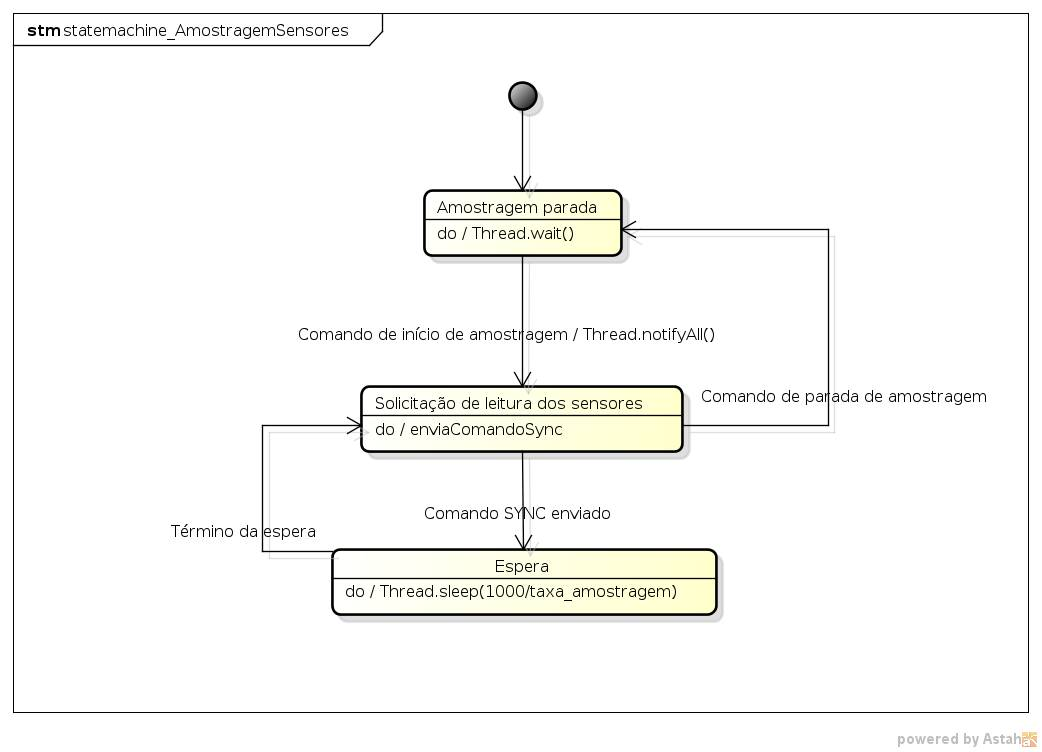
\includegraphics[width=\textwidth, keepaspectratio]{./figuras/sistEmbarcado/statemachine_AmostragemSensores_sistEmbarcado.jpg}
  \caption{Diagrama de estados da \textit{thread} responsável por efetuar a amostragem dos sensores (linux embarcado).}
  \label{fig:diagrama_estados_amostragem_sensores_sist_embarcado}
\end{figure}

\begin{figure}[H]
  \centering
  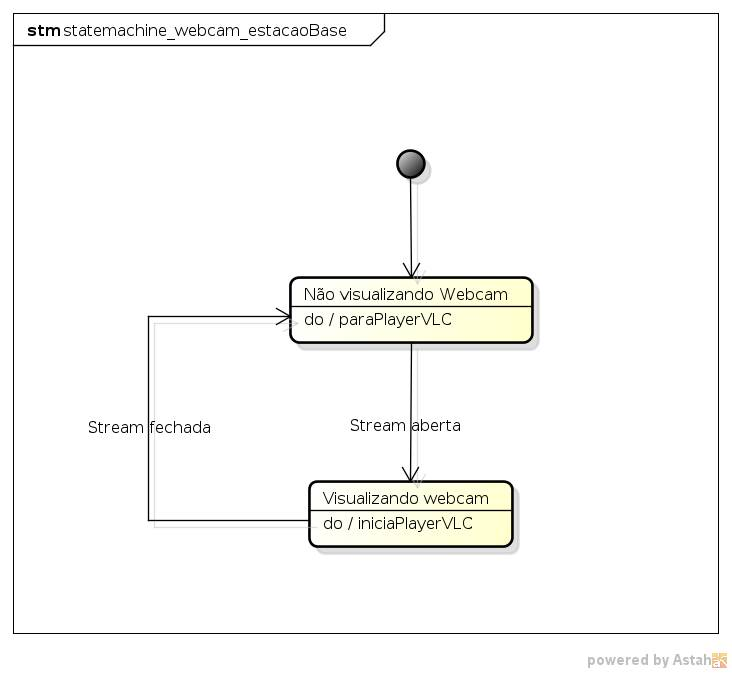
\includegraphics[width=\textwidth, keepaspectratio]{./figuras/estacaoBase/statemachine_webcam_estacaoBase.jpg}
  \caption{Diagrama de estados do visualização de imagens da \textit{webcam} (estação base).}
  \label{fig:diagrama_estados_webcam_estacao_base}
\end{figure}

\begin{figure}[H]
  \centering
  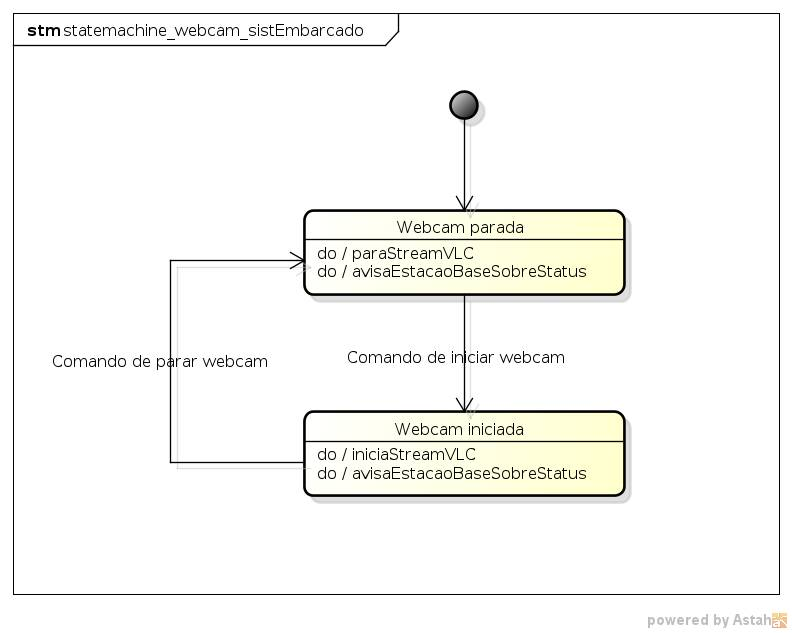
\includegraphics[width=\textwidth, keepaspectratio]{./figuras/sistEmbarcado/statemachine_webcam_sistEmbarcado.jpg}
  \caption{Diagrama de estados do envio de imagens da \textit{webcam} (linux embarcado).}
  \label{fig:diagrama_estados_webcam_sist_embarcado}
\end{figure}



\subsection{Diagramas de sequência}

Nessa seção os diagramas de sequência de comandos dos motores, de mensagens de amostras dos sensores e da ativação da webcam. Os diagramas das Figuras \ref{fig:diagrama_sequencia_motores_estacao_base} e \ref{fig:diagrama_sequencia_motores_sist_embarcado} representam como um comando de mudança de velocidade das rodas dado pelo usuário chega até a placa de baixo nível. Os das Figuras \ref{fig:diagrama_sequencia_sensores_sist_embarcado} e \ref{fig:diagrama_sequencia_sensores_estacao_base} demonstram a sequência dos dados de leituras dos sensores que saem da placa de baixo nível e chegam até o usuário.  Os diagramas das Figuras \ref{fig:diagrama_sequencia_webcam_estacao_base} e \ref{fig:diagrama_sequencia_webcam_sist_embarcado} demonstram um comando de ativação da webcam dado pelo usuário, como ele chega até o Linux embarcado e como posteriormente o usuário recebe as imagens da webcam.

Vale ressaltar que as chamadas assíncronas, ou seja, que não bloqueiam a execução da \textit{thread} chamadora, foram representadas também nestes diagramas.

\begin{figure}[H]
  \centering
  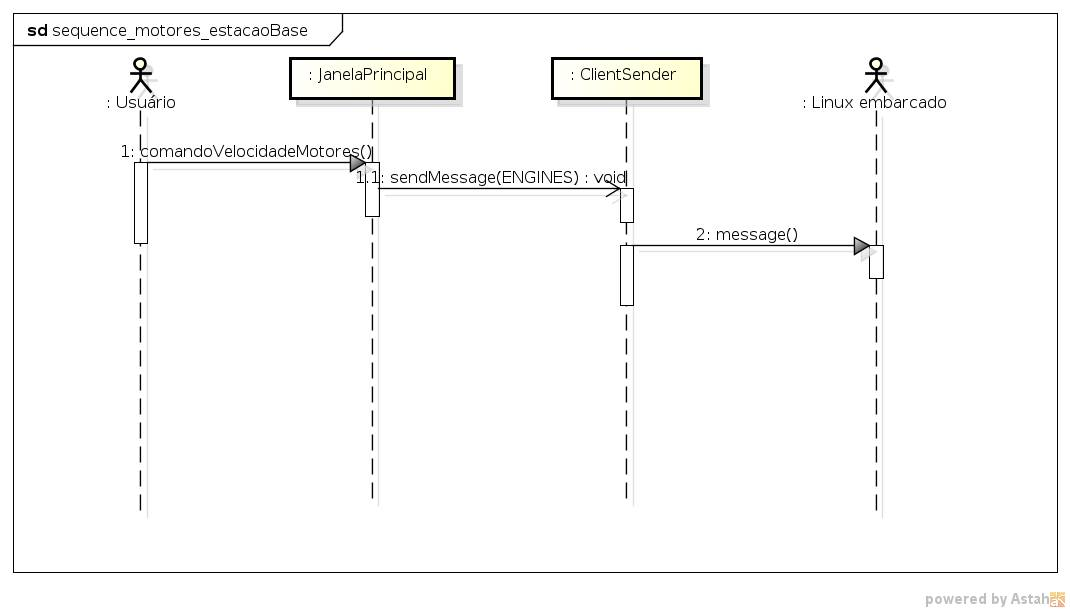
\includegraphics[width=\textwidth, keepaspectratio]{./figuras/estacaoBase/sequence_motores_estacaoBase.jpg}
  \caption{Diagrama de sequência de comando para mudança de velocidade dos motores (representa comando dado pelo usuário).}
  \label{fig:diagrama_sequencia_motores_estacao_base}
\end{figure}

\begin{figure}[H]
  \centering
  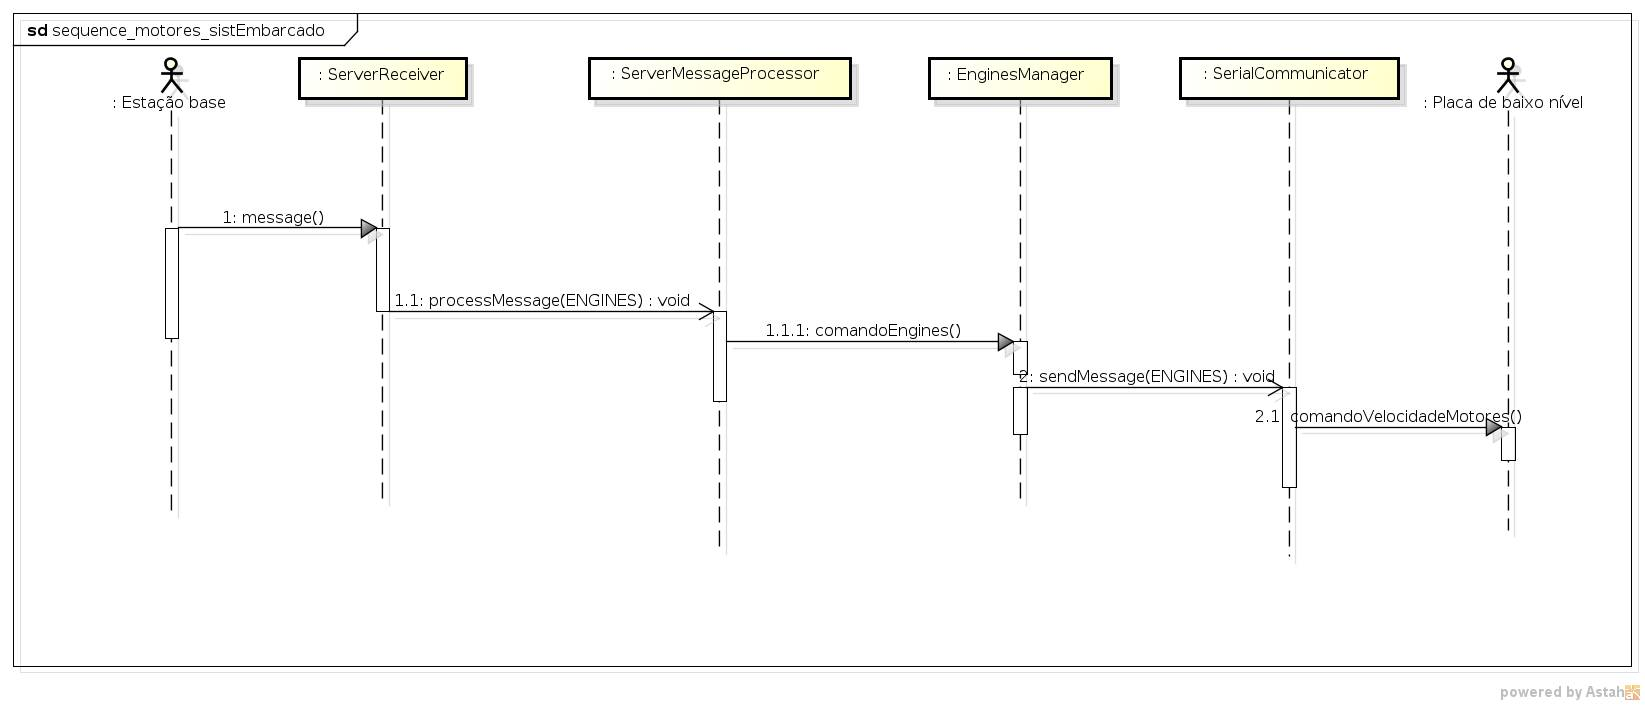
\includegraphics[width=\textwidth, keepaspectratio]{./figuras/sistEmbarcado/sequence_motores_sistEmbarcado.jpg}
  \caption{Diagrama de sequência de comando para mudança de velocidade dos motores (representa mensagem chegando no sistema embarcado).}
  \label{fig:diagrama_sequencia_motores_sist_embarcado}
\end{figure}

\begin{figure}[H]
  \centering
  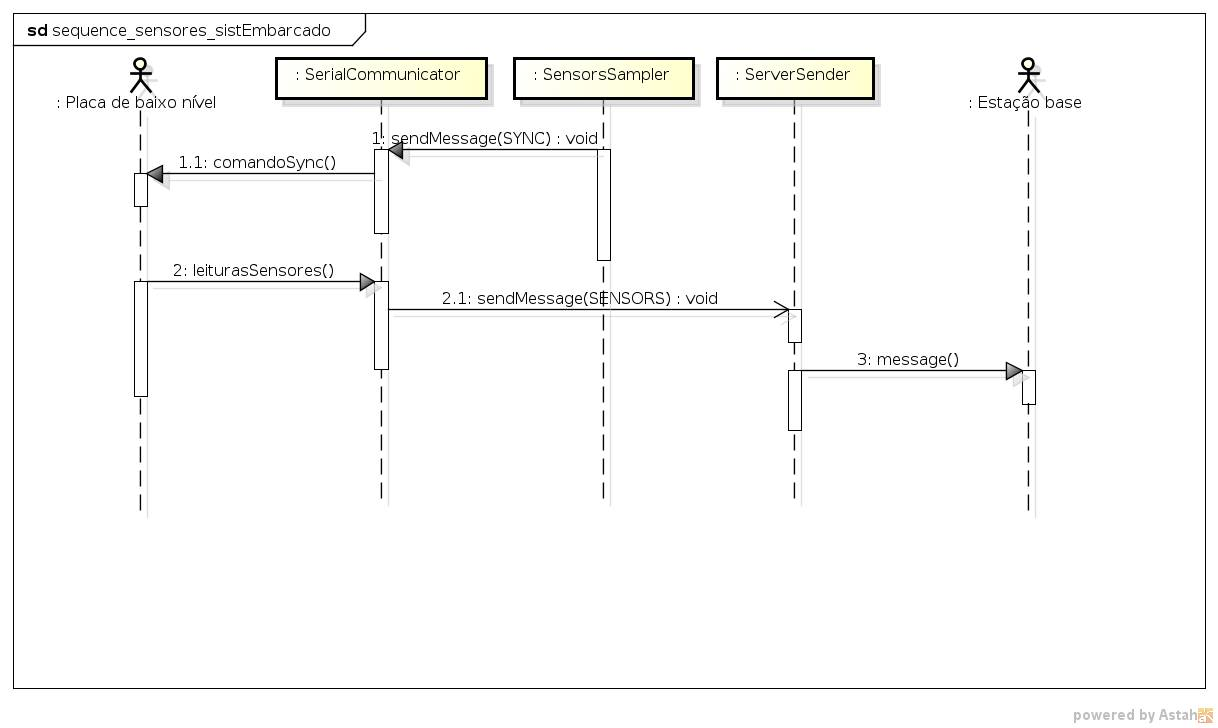
\includegraphics[width=\textwidth, keepaspectratio]{./figuras/sistEmbarcado/sequence_sensores_sistEmbarcado.jpg}
  \caption{Diagrama de sequência da amostragem dos sensores (representa amostras saindo do sistema embarcado).}
  \label{fig:diagrama_sequencia_sensores_sist_embarcado}
\end{figure}

\begin{figure}[H]
  \centering
  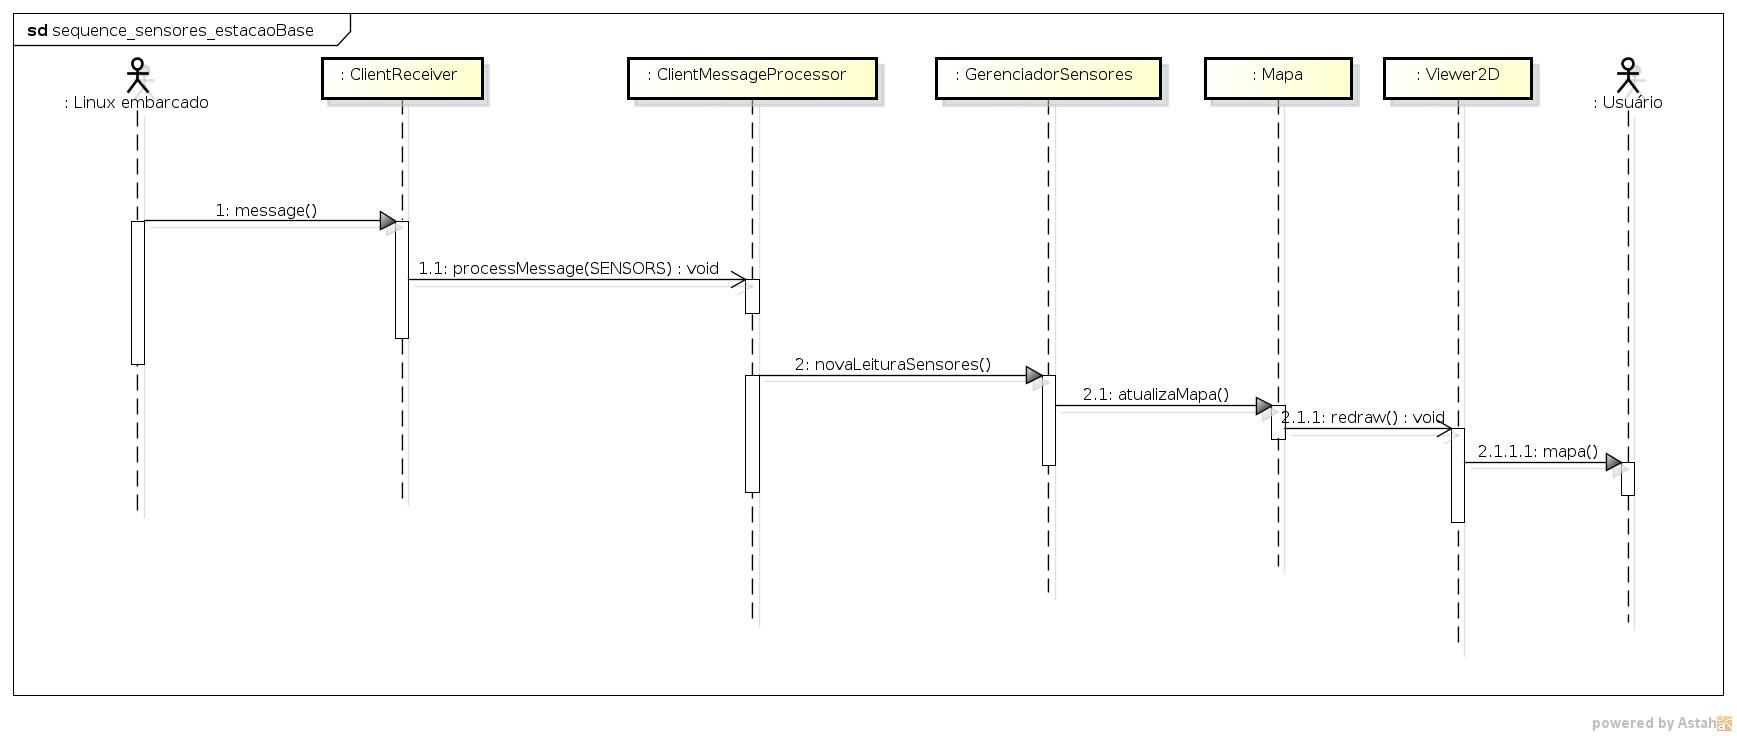
\includegraphics[width=\textwidth, keepaspectratio]{./figuras/estacaoBase/sequence_sensores_estacaoBase.jpg}
  \caption{Diagrama de sequência da amostragem dos sensores (representa mensagem chegando na estação base).}
  \label{fig:diagrama_sequencia_sensores_estacao_base}
\end{figure}

\begin{figure}[H]
  \centering
  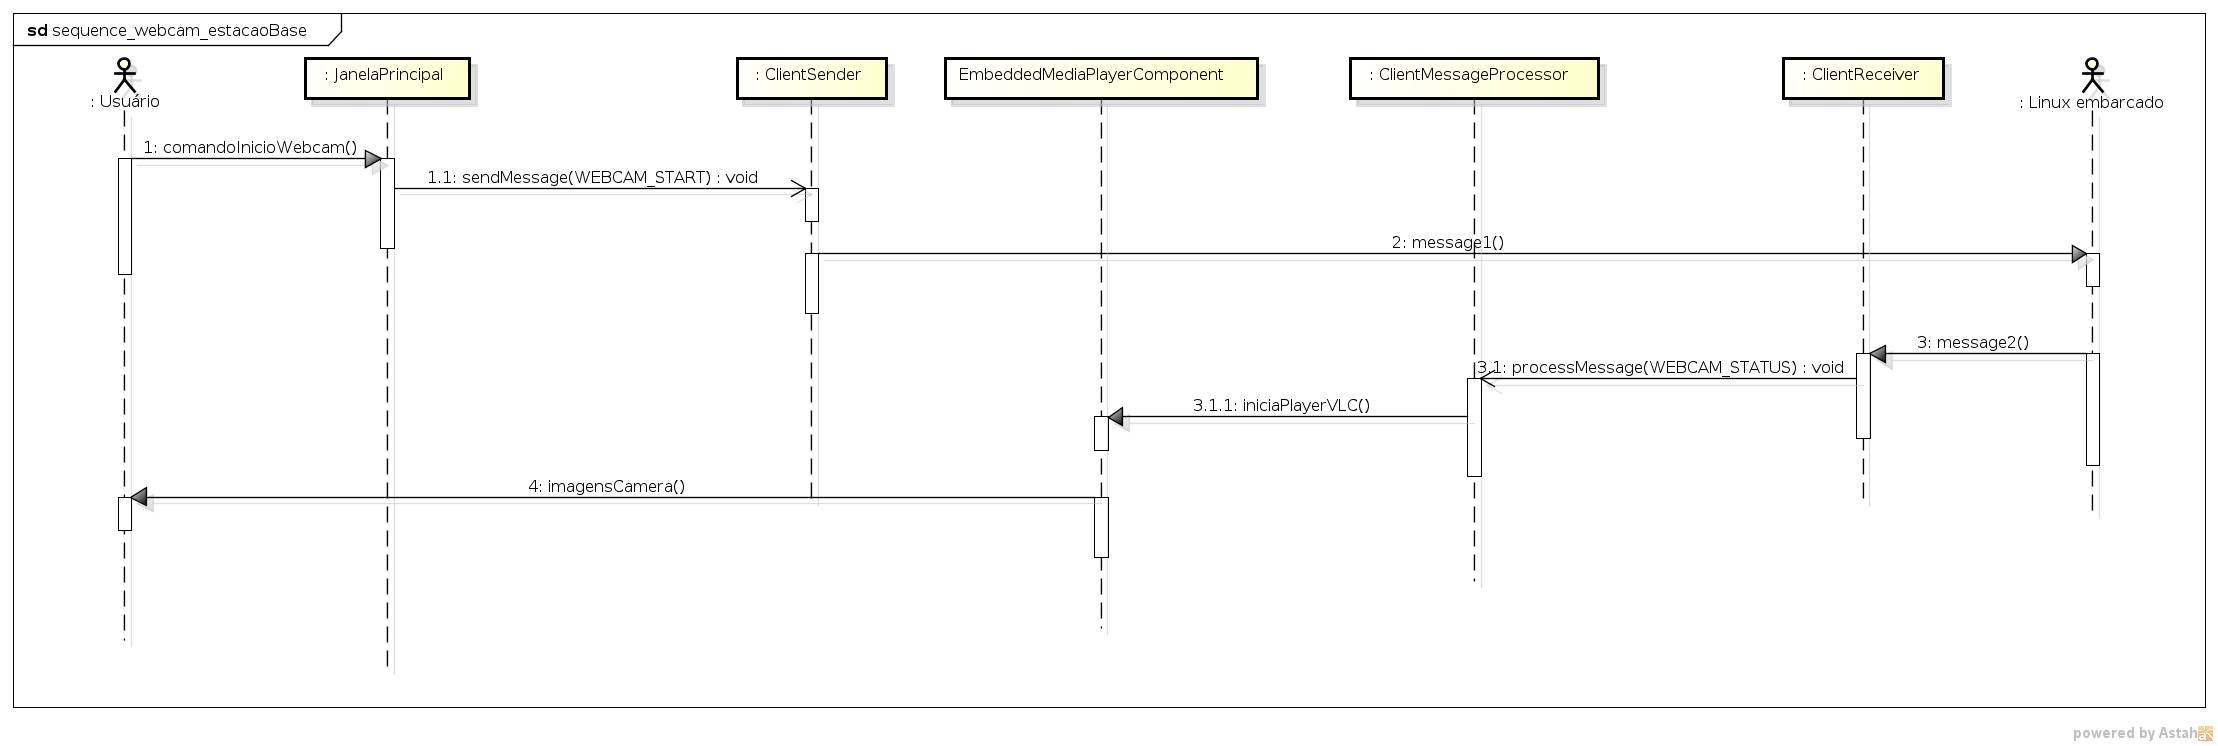
\includegraphics[width=\textwidth, keepaspectratio]{./figuras/estacaoBase/sequence_webcam_estacaoBase.jpg}
  \caption{Diagrama de sequência de comando para ativação da webcam (representa comando dado pelo usuário e o \textit{player} da \textit{libVLC} sendo ativado posteriormente).}
  \label{fig:diagrama_sequencia_webcam_estacao_base}
\end{figure}

\begin{figure}[H]
  \centering
  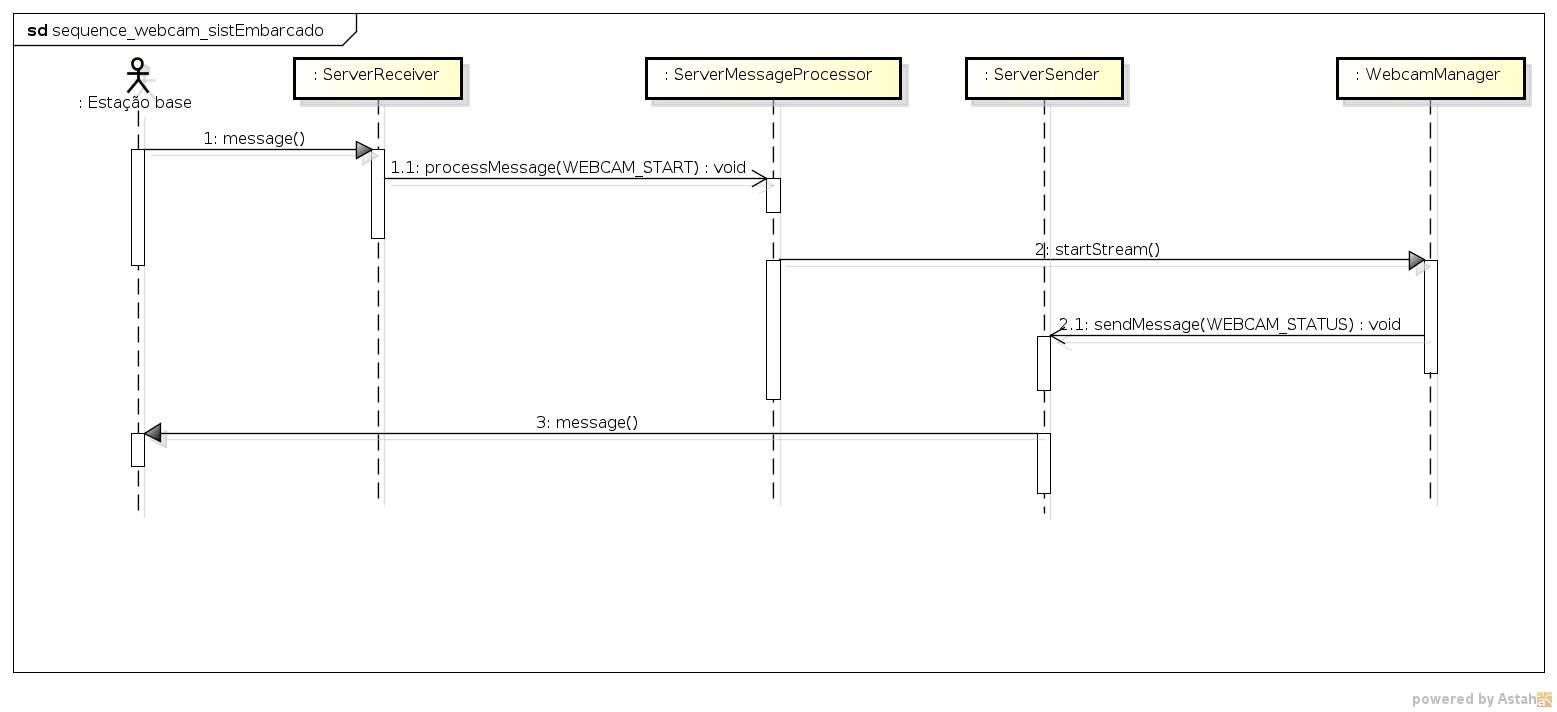
\includegraphics[width=\textwidth, keepaspectratio]{./figuras/sistEmbarcado/sequence_webcam_sistEmbarcado.jpg}
  \caption{Diagrama de sequência de comando para ativação da webcam (representa mensagem de ativação da webcam chegando no sistema embarcado e estação base sendo posteriormente notificada sobre o novo status).}
  \label{fig:diagrama_sequencia_webcam_sist_embarcado}
\end{figure}




\chapter{Diagrama de blocos do hardware}
Na figura \ref{fig:diagrama_blocos_hardware} mostra-se o diagrama de blocos do sistema embarcado e suas conexões com o restante do robô. A seguir está também uma descrição para cada um dos blocos da placa de circuito impresso do sistema embarcado.

\begin{figure}[H]
  \centering
  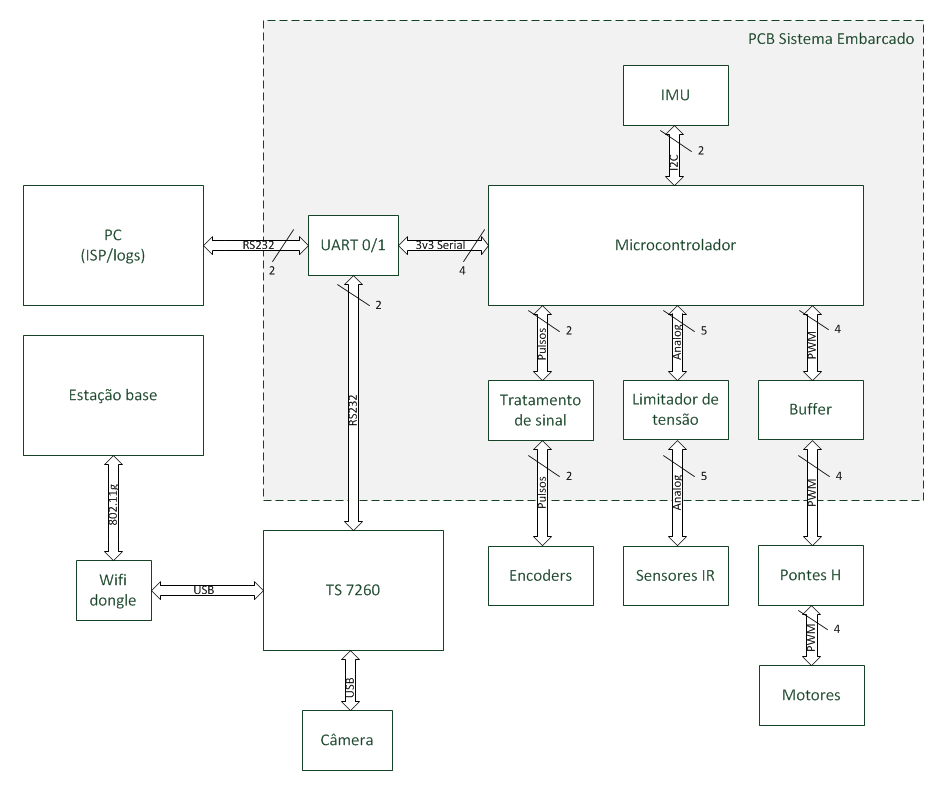
\includegraphics[width=\textwidth]{./figuras/diagrama_blocos_hardware.png}
  \caption{Diagrama de blocos do hardware}
  \label{fig:diagrama_blocos_hardware}
\end{figure}


\begin{enumerate}[topsep=0pt, partopsep=0pt, itemsep=0pt]
    \item Microcontrolador: Este bloco fará a leitura dos sensores: encoders, infra-vermelhos, acelerômetro e giroscópios. Além disso possui a implementação do protocolo de comunicação para interação com o linux embarcado da placa TS-7260.
    \item UART 0/1: Responsável por ajustar os níveis de tensão para comunicação serial no padrão RS-232 com a placa TS-7260.
    \item Buffer: Responsável por fornecer corrente e elevar os níveis de tensão de saída do microcontrolador de 3,3V para 5,0V. Esse buffer é conectado às pontes H já existentes no robô.
    \item IMU: possui o acelerômetro e o giroscópio e se comunicará com o microcontrolador por meio do protocolo I2C.
    \item Limitador de tensão: Necessário pois os sinais de saída dos sensores de infravermelho que já existem no robô não estão limitados em 5V, podendo a saída ultrapassar 5,0V e danificar o microcontrolador. 
    \item Tratamento de sinal: Composto por um filtro RC passa baixas e um schmitt trigger para remover qualquer falha que possa ocorrer na geração dos pulsos no encoder. A frequência de corte do filtro pode ser obtida pela velocidade máxima que o robô pode atingir, que foi suposta em 1 m/s (como apresentado nos requisitos de hardware).
\end{enumerate}



\chapter{Interface gráfica da estação base}

A interface gráfica desenvolvida para a estação base está representada nas Figuras \ref{fig:interface_estacao_base1} e \ref{fig:interface_estacao_base2}. O usuário tem acesso na janela principal aos recursos básicos, como imagem da webcam, controles de movimentação do robô e visualização do mapa.
A parte de visualização 2D do mapa (a maior área da janela principal) foi desenvolvida a partir da biblioteca do Processing. O visualizador 2D (classe \textit{Viewer2D} apresentada anteriormente) possui recursos de arraste, \textit{zoom} e rotação, desenvolvidos a partir do zero pela equipe. O usuário pode salvar e carregar os mapas criados com o robô através dos botões do canto superior esquerdo da janela. A conexão com o robô pode ser feita rapidamente com o botão ``Conexão'', e o controle de gravação do mapa e recebimento de dados dos sensores e da webcam pode ser feito a utilizando-se dos dois botões logo a seguir. Com o botão ``Reposicionar'', o usuário pode efetuar o reposicionamento do robô no mapa. 

O botão ``Avançado'' abre uma janela que possui recursos de configuração e utilização avançada, o que inclui alteração dos parâmetros de ajuste fino, como média móvel dos sensores IR e limiares de aceleração e velocidade angular. Além disso, está presente um recurso bastante útil que é o de salvar em um arquivo amostras dos sensores da maneira que são recebidas (sem nenhum tratamento adicional). O programa e o algoritmo de criação do mapa podem ser alterados, e essas amostras podem ser posteriormente carregadas para efetuar testes das alterações feitas. Vale ressaltar que, no decorrer do projeto, esse foi um recurso que melhorou o rendimento da equipe, pois dessa forma testes práticos com o robô não necessitavam ser repetidos continuamente para testar modificações no programa.

\begin{figure}[H]
	\centering
	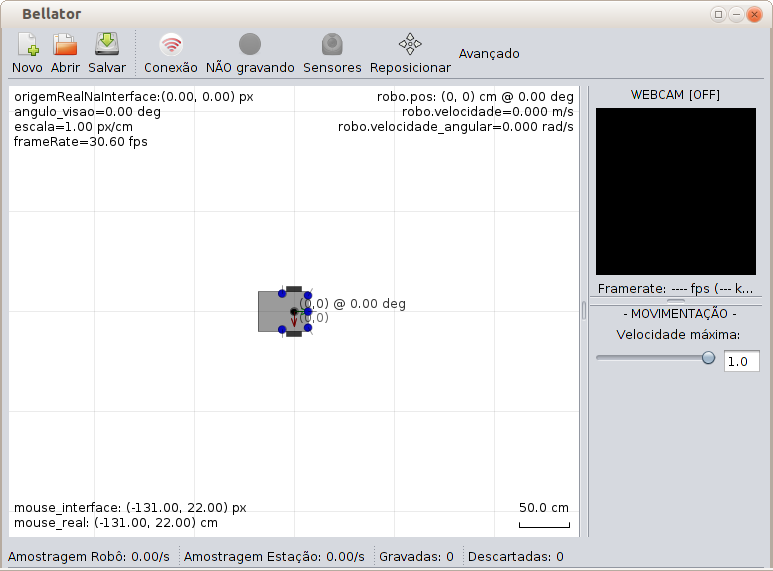
\includegraphics[width=1\textwidth]{./figuras/estacaoBase/interface_estacao_base1.png}
	\caption{Janela principal da interface gráfica da estação base.}
	\label{fig:interface_estacao_base1}
\end{figure}
\begin{figure}[H]
	\centering
	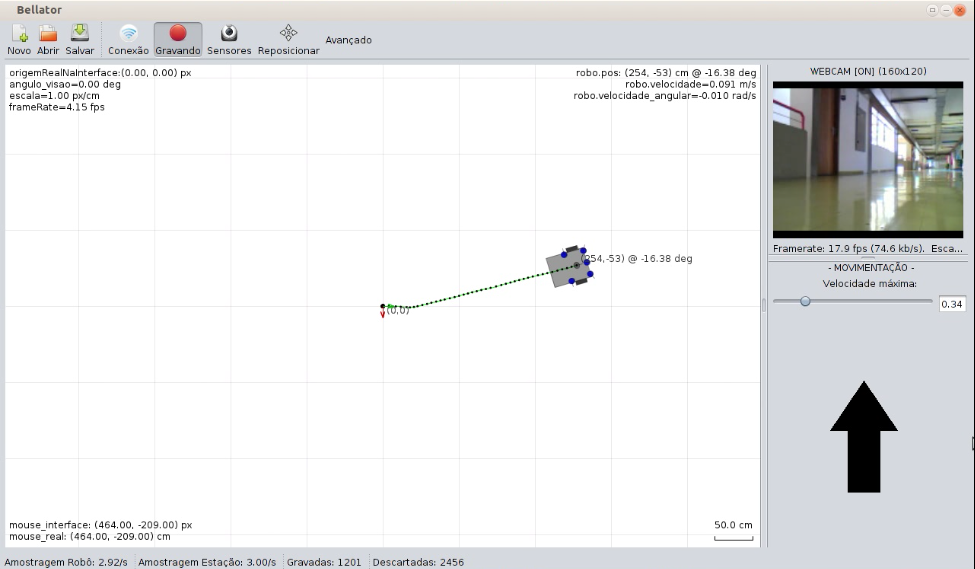
\includegraphics[width=1\textwidth]{./figuras/estacaoBase/interface_estacao_base2.png}
	\caption{Estação base em utilização na prática.}
	\label{fig:interface_estacao_base2}
\end{figure}
\chapter{Geração do mapa}

A posição do robô no mapa em cada instante é representada por um ponto no plano cartesiano e por um ângulo, que indica para qual sentido o robô está orientado. Esse ponto no plano indica onde está o centro de movimento do robô, que é o ponto médio entre as duas rodas.

Neste projeto, a determinação do deslocamento do robô é determinada primariamente pelos encoders presentes cada roda. O acelerômetro e o giroscópio são utilizados para aumentar a confiabilidade dos cálculos de deslocamento, principalmente em caso de escorregamento das rodas.

Na próxima seção será explicada a teoria da determinação do deslocamento, velocidade e aceleração do centro de movimento do robô a partir das leituras dos encoders em cada instante. Na seção \ref{sec:teoria_acel_giro} será explicitada a forma como as leituras do acelerômetro e giroscópio serão utilizadas para aumentar a confiabilidade das medições.

Na Figura \ref{fig:robo} está presente um esquema básico do robô visto de cima e virado com a frente para a direita. Nessa figura estão presentes os nomes das variáveis que são utilizadas nos cálculos posteriores.

\begin{figure}[H]
  \centering
  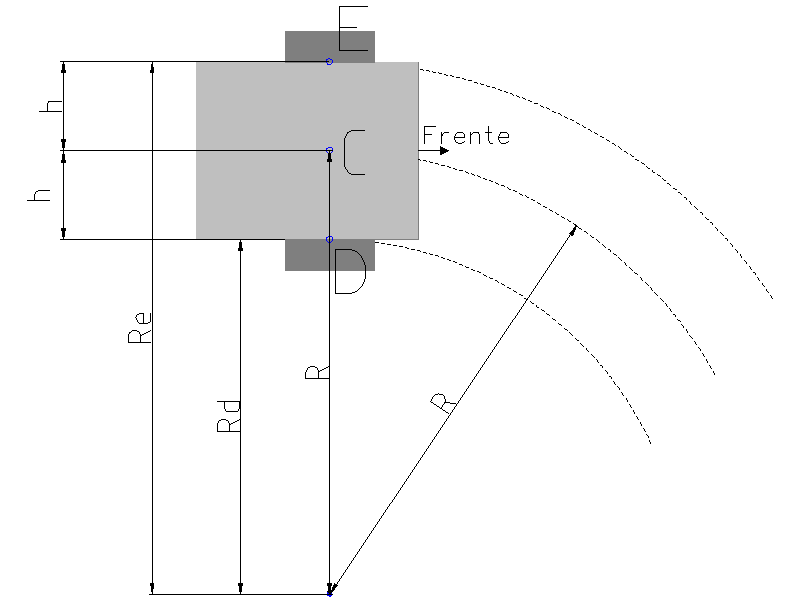
\includegraphics[width=0.5\textwidth, keepaspectratio]{./figuras/robo/robo.png}
  \caption{Representação básica do robô (visão superior).}
  \label{fig:robo}
\end{figure}

\section{Encoders}

Há dois dados importantes a determinar sobre o deslocamento do centro de movimento do robô: o deslocamento linear (distância absoluta percorrida) e o angular (variação do ângulo de orientação do robô). Cada encoder fornece uma medida de contagem de pulsos por volta a cada intervalo de amostragem. 

Na Figura \ref{fig:roda_encoder} está presente um representação básica de uma roda, acoplada a um encoder. Os números da figura são utilizados como índices nos cálculos explicitados posteriormente.

\begin{figure}[H]
  \centering
  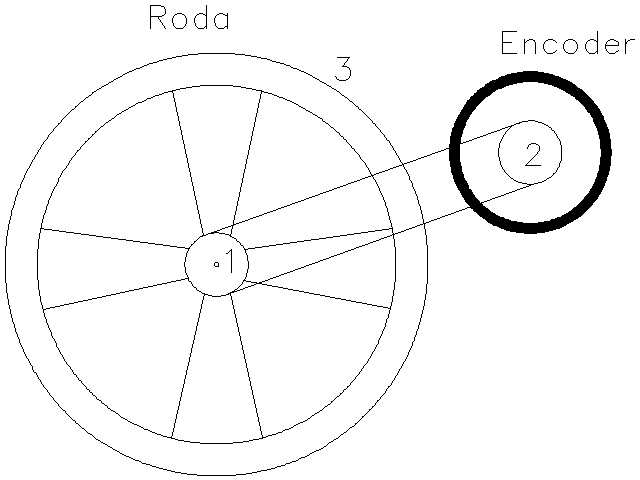
\includegraphics[width=0.5\textwidth, keepaspectratio]{./figuras/robo/roda_encoder.png}
  \caption{Representação de uma roda acoplada a um encoder.}
  \label{fig:roda_encoder}
\end{figure}

\subsection{Deslocamento de cada roda}

Um princípio importante utilizado nos cálculos é a relação entre o deslocamento $\Delta x$ ao redor de uma circunferência (de raio $R$) e a variação do ângulo $\Delta \theta$:

\begin{equation}
  \Delta x = R \cdot \Delta \theta
  \label{eq:deslocamento_circunferencia}
\end{equation}

Nos cálculos a seguir, faz-se uso do índice 1 para o eixo da roda, 2 para o eixo do encoder e 3 para a própria roda, de acordo com a figura \ref{fig:roda_encoder}. Para determinar a distância percorrida pela roda, deve-se considerar a circunferência do eixo da roda ($C_1$), a circunferência do eixo do encoder ($C_2$) e a circunferência da roda ($C_3$).

O acoplamento do eixo do encoder com o eixo da roda é feita por uma correia de borracha, e portanto considera-se que o deslocamento ($ \Delta x_1$) na superfície do eixo da roda é igual ao deslocamento ($ \Delta x_2$) na superfície do eixo do encoder. Pode-se, com isso, calcular:

\begin{eqnarray*}
   \Delta x_1 =  \Delta x_2 \rightarrow \Delta \theta_1 R_1 = \Delta \theta_2 R_2 \rightarrow \Delta \theta_1 \frac{C_1}{2 \pi} = \Delta \theta_2 \frac{C_2}{2 \pi} 
\end{eqnarray*}

\begin{equation}
  \Delta \theta_1 = \frac{C_2}{C_1} \cdot \Delta \theta_2
  \label{eq:theta1_theta2}
\end{equation}

Calculando-se a relação entre a contagem de pulsos do encoder ($E$) e o ângulo de rotação ($\Delta \theta_2$) do eixo do encoder, levando-se em conta que há uma contagem de 1800 pulsos por volta:

\begin{equation}
  \Delta \theta_2 = \frac{2 \pi}{1800} \cdot E \unit{rad}
  \label{eq:E_theta2}
\end{equation}

Substituindo-se a equação \ref{eq:E_theta2} na \ref{eq:theta1_theta2}, tem-se que:

\begin{equation}
  \Delta \theta_1 = \frac{C_2}{C_1} \frac{2 \pi}{1800} \cdot E \unit{rad}
  \label{eq:theta_1}
\end{equation}

Calculando-se a relação entre a variação do ângulo do eixo da roda ($\Delta \theta_1$) e o deslocamento da roda ($x_3$):

\begin{eqnarray*}
  \Delta \theta_1 = \Delta \theta_3 \rightarrow \Delta \theta_1 =  \Delta x_3 R_3 \rightarrow \Delta \theta_1 = \Delta x_3 \frac{C_3}{2 \pi} \rightarrow  \Delta x_3 = \Delta \theta_1 \frac{2 \pi}{C_3}
\end{eqnarray*}

Substituindo-se o valor de ($\Delta \theta_1$) da equação \ref{eq:theta_1}:

\begin{eqnarray*}
   \Delta x_3 = \frac{C_2}{C_1} \frac{2 \pi}{1800} \cdot E \cdot \frac{2 \pi}{C_3} = \frac{C_2}{C_1 C_3} \frac{(2 \pi)^2}{1800} \cdot E
\end{eqnarray*}

\begin{empheq}[box=\fbox]{equation}
   \Delta x_3 = \frac{C_2}{C_1 C_3} \frac{\pi^2}{450} \cdot E
  \label{eq:x_3}
\end{empheq}


Que é o valor do deslocamento da roda em função da contagem de pulsos do encoder. 


\subsection{Deslocamento do centro de movimento do robô}

Como já explicitado anteriormente, o centro de movimento do robô considerado é o ponto médio entre as duas rodas. As duas variáveis para determinar em cada instante de tempo são o deslocamento linear (distância absoluta percorrida) e o angular (variação do ângulo de orientação do robô). Considerando-se que em cada instante o robô descreve um movimento circular uniforme (MCU), o raio da trajerória deve ser determinado para que os cálculos de posicionamento do robô possam ser feitos. Este raio depende do deslocamento das rodas em cada instante, e é uma importante variável que será estudada na próxima subseção.

Nos cálculos que serão explicitados a seguir, utiliza-se o índice E para a roda esquerda, C para o centro de movimento do robô e D para a roda direita.

Uma relação importante a notar a princípio é que a variação do ângulo de orientação em cada instante é igual nos três pontos: E (roda esquerda), C (centro de movimento) e D (roda direita), visto que todos estão fixos em relação à carcaça do robô. Parte-se da seguinte relação fundamental, portanto:

\begin{equation}
  \Delta \theta_E = \Delta \theta_D = \Delta \theta_C
  \label{eq:relacao_fundamental_theta}
\end{equation}



\subsubsection{Raio do movimento}

Para determinar o raio ($R$) descrito pelo centro de movimento do robô em sua trajetória instantânea em MCU, usa-se os dois primeiros termos da igualdade da equação \ref{eq:relacao_fundamental_theta}:

\begin{eqnarray*}
  \Delta \theta_E = \Delta \theta_D \rightarrow \frac{\Delta x_E}{R_E} = \frac{\Delta x_D}{R_D} 
\end{eqnarray*}

Mas:
\begin{equation*}
  R_E = R + h, ~ ~ R_D = R - h
\end{equation*}

Portanto:

\begin{eqnarray*}
  \frac{\Delta x_E}{R + h} = \frac{\Delta x_D}{R - h} ~\rightarrow~ \frac{\Delta x_E}{\Delta x_D} = \frac{R + h}{R - h} ~\rightarrow~ \frac{\Delta x_E (R - h)}{\Delta x_D} = R + h 
\end{eqnarray*}
\begin{eqnarray*}
  \frac{\Delta x_E \cdot R - \Delta x_E \cdot h}{\Delta x_D} = R + h ~\rightarrow~ 
  \frac{\Delta x_E}{\Delta x_D} \cdot R - \frac{\Delta x_E}{\Delta x_D} \cdot h = R + h ~\rightarrow~ 
  \frac{\Delta x_E}{\Delta x_D} \cdot R - R = \frac{\Delta x_E}{\Delta x_D} \cdot h + h
\end{eqnarray*}
\begin{eqnarray*}
  R \left( \frac{\Delta x_E}{\Delta x_D} - 1 \right) = h \left( \frac{\Delta x_E}{\Delta x_D} + 1 \right) ~\rightarrow~
  R = h \cdot \frac{\left( \frac{\Delta x_E}{\Delta x_D} + 1 \right)}{\left( \frac{\Delta x_E}{\Delta x_D} - 1 \right)}  ~\rightarrow~
  R = h \cdot \frac{\frac{\Delta x_E + \Delta x_D}{x_D}}{\frac{\Delta x_E - \Delta x_D}{\Delta x_D}} 
\end{eqnarray*}

\begin{empheq}[box=\fbox]{equation}
  R = h \cdot \frac{\Delta x_E + \Delta x_D} {\Delta x_E - \Delta x_D}
  \label{eq:R}
\end{empheq}

Vê-se que o raio $R$ do movimento circular uniforme em cada instante depende do deslocamento de cada roda ($\Delta x_E$ e $\Delta x_D$) e da distãncia $h$ entre as rodas e o centro de movimento do robô.


\subsubsection{Deslocamento linear} 

Para calcular o deslocamento linear do centro de movimento do robô, usa-se os dois últimos termos da equação \ref{eq:relacao_fundamental_theta}. Vale ressaltar que poderiam ser escolhidos também o primeiro e o último termos, pois o resultado obtido seria idêntico. Tem-se que:

\begin{eqnarray*}
  \Delta \theta_D = \Delta \theta_C \rightarrow \frac{\Delta x_D}{R_D} = \frac{\Delta x_C}{R} 
\end{eqnarray*}

Mas:
\begin{equation*}
  R_D = R - h
\end{equation*}

Portanto:
\begin{eqnarray*}
  \frac{\Delta x_D}{R - h} = \frac{\Delta x_C}{R} ~\rightarrow~ x_D = x_C \cdot \frac{R - h}{R} 
\end{eqnarray*}

Substituindo-se o valor de $R$ da equação \ref{eq:R}:
\begin{eqnarray*}
  \Delta x_D = \Delta x_C \left[ \frac{h \cdot \frac{\Delta x_E + \Delta x_D}{\Delta x_E - \Delta x_D} - h}{h \cdot \frac{\Delta x_E + \Delta x_D}{\Delta x_E - \Delta x_D}} \right]
\end{eqnarray*}

Dividindo-se o numerador e denominador do segundo termo por $h$:
\begin{equation*}
  \Delta x_D = \Delta x_C \left[ \frac{\frac{\Delta x_E + \Delta x_D}{\Delta x_E - \Delta x_D} - 1}{\frac{\Delta x_E + \Delta x_D}{\Delta x_E - \Delta x_D}} \right]
\end{equation*}

Multiplicando-se o numerador e denominador do segundo termo por $\frac{\Delta x_E - \Delta x_D}{\Delta x_E + \Delta x_D}$:

\begin{equation*}
  \Delta x_D = \Delta x_C \left[1 - \frac{\Delta x_E - \Delta x_D}{\Delta x_E + \Delta x_D} \right] ~\rightarrow~
  \Delta x_D = \Delta x_C \left[\frac{(\Delta x_E + \Delta x_D) - (\Delta x_E - \Delta x_D)}{\Delta x_E + \Delta x_D} \right] 
\end{equation*}
\begin{equation*}
  \Delta x_D = \Delta x_C \cdot \left[ \frac{2 \Delta x_D}{\Delta x_E + \Delta x_D} \right] ~\rightarrow~
  \Delta x_C = \frac{\Delta x_D}{\left(\frac{2 \Delta x_D}{\Delta x_E + \Delta x_D} \right)}
\end{equation*}

\begin{empheq}[box=\fbox]{equation}
  \Delta x_C = \frac{\Delta x_E + \Delta x_D}{2}
  \label{eq:desloc_linear}
\end{empheq}

Notas-se que o deslocamento linear do centro de movimento do robô ($\Delta x_C$) é uma média simples dos dois deslocamentos lineares das rodas. Vê-se que ele não depende do raio de deslocamento nem da distância entre as duas rodas.


\subsubsection{Deslocamento angular}

O deslocamento angular ($\Delta \theta_c$) do centro de movimento do robô em cada instante pode ser calculado a partir do deslocamento linear e do raio do movimento circular uniforme. Usando-se a relação da equação \ref{eq:deslocamento_circunferencia}, tem-se que:


\begin{empheq}[box=\fbox]{equation}
  \Delta \theta_c = \frac{\Delta x_C}{R}
  \label{eq:desloc_angular}
\end{empheq}


Onde $\Delta x_C$ é o deslocamento linear do robô (equação \ref{eq:desloc_linear}) e $R$ é o raio do movimento circular uniforme (equação \ref{eq:R}). 

\subsubsection{Casos especiais}

Há dois casos especiais que devem ser considerados no cálculo do deslocamento (a partir dos dados dos encoders) do centro de movimento do robo. O primeiro é quando as duas rodas têm deslocamento igual ($\Delta x_E = \Delta x_D$). O raio do movimento circular (equação \ref{eq:R}) neste caso é:

\begin{equation}
  R = h \cdot \frac{\Delta x_E + \Delta x_D} {\Delta x_E - \Delta x_D} = h \cdot \frac{2 \cdot \Delta x_E}{0} \rightarrow \infty
  \label{eq:caso_especial1_R}
\end{equation}


O raio tende a infinito, o que implica que o deslocamento angular (equação \ref{eq:desloc_angular}) seja:

\begin{equation}
  \Delta \theta_c = \frac{\Delta x_C}{R} = \frac{\Delta x_C}{\infty} \rightarrow 0
  \label{eq:caso_especial1_theta}
\end{equation}

Já o deslocamento linear (equação \ref{eq:desloc_linear}) é:

\begin{equation}
  \Delta x_C = \frac{\Delta x_E + \Delta x_D}{2} = \frac{2 \Delta x_E}{2} = \Delta x_E
  \label{eq:caso_especial1_x}
\end{equation}

Isso corresponde à realidade, uma vez que quando as rodas têm deslocamentos iguais o robô está se deslocando sem fazer curvas. Não há deslocamento angular, portanto, e o deslocamento linear do centro de movimento é igual ao deslocamento de cada roda.

O segundo caso especial ocorre quando os deslocamento têm módulos iguais, porêm sentidos contrários (ou seja, $\Delta x_E = - \Delta x_D$). O raio nesse caso é:

\begin{equation}
  R = h \cdot \frac{\Delta x_E + \Delta x_D} {\Delta x_E - \Delta x_D} = h \cdot \frac{\Delta x_E - \Delta x_E}{\Delta x_E + \Delta x_E} = 0
    \label{eq:caso_especial2_R}
\end{equation}


O deslocamento linear (equação \ref{eq:desloc_linear}) é:

\begin{equation}
  \Delta x_C = \frac{\Delta x_E + \Delta x_D}{2} = \frac{\Delta x_E - \Delta x_E}{2} = 0
  \label{eq:caso_especial2_x}
\end{equation}

Esse valor corresponde à realidade, pois quando as rodas se deslocam em sentidos contários, e na mesma quantidade, o centro de movimento do robô não se desloca linearmente, mas apenas muda seu ângulo.
Usando-se a equação \ref{eq:desloc_angular}, tenta-se calcular o valor do deslocamento angular:

\begin{equation}
  \Delta \theta_c = \frac{\Delta x_C}{R} = \frac{0}{0}
  \label{eq:caso_especial2_theta}
\end{equation}

O valor obtido é indeterminado quando usa-se essa equação. Porém, analisando-se a natureza deste caso especial, pode ser notado que há um movimento circular cujo centro é o ponto médio entre as rodas (que é o centro de movimento do robô). O raio do MCU é a distância $h$ entre uma roda e o centro do robô, e o deslocamento ao longo da circunferência é o deslocamento de qualquer uma uma das rodas. Portanto, a equação \ref{eq:deslocamento_circunferencia} pode ser utilizada, isolando-se a variável $\theta$, para determinar o deslocamento angular do robô:

\begin{equation}
  \Delta \theta_c = \frac{\Delta x_E}{h}
  \label{eq:caso_especial2_theta2}
\end{equation}


\subsubsection{Velocidade e aceleraçao}

A velocidade e aceleração lineares do centro de movimento do robô podem ser calculadas por derivação numérica do deslocamento e velocidade em cada intervalo de tempo, considerando-se a velocidade e aceleração anteriores. Em cada intervalo discreto $n$:

\begin{equation}
  v_{c (n)} = \frac{x_{c (n)} - x_{c (n-1)}}{t_{(n)} - t_{(n-1)}}
  \label{eq:velocidade}
\end{equation}

\begin{equation}
  a_{c (n)} = \frac{v_{c (n)} - v_{c (n-1)}}{t_{(n)} - t_{(n-1)}}
  \label{eq:velocidade}
\end{equation}


A velocidade e aceleração angulares podem ser também obtidas por derivação numérica, considerando-se que o raio do movimento circular uniforme do robô é constante dentro do intervalo considerado. Em cada intervalo discreto $n$:

\begin{equation}
  \omega_{c (n)} = \frac{\theta_{c (n)} - \theta_{c (n-1)}}{t_{(n)} - t_{(n-1)}}
  \label{eq:velocidade}
\end{equation}

\begin{equation}
  \alpha_{c (n)} = \frac{\omega_{c (n)} - \omega_{c (n-1)}}{t_{(n)} - t_{(n-1)}}
  \label{eq:velocidade}
\end{equation}


\section{Acelerômetro e giroscópio}
\label{sec:teoria_acel_giro}

O acelerômetro e o giroscópio são utilizados para aumentar a confiabilidade dos dados de deslocamento do robô em caso de escorregamento das rodas.



Como definido na seção \ref{sec:codificacao_mensagens}, é recebido um valor de 2 bytes para cada eixo do acelerômetro. A faixa de funcionamento do acelerômetro está configurada em $-+2g$, logo a sensibilidade pelo \textit{datasheet} é de $16384 LSB/g$. Portanto, o valor de aceleração pode ser obtido pela fórmula:

\begin{equation}
  a = \frac{valorMedido}{16384} \cdot g \unit{m/s^2}
  \label{eq:acel}
\end{equation}

Onde g é a aceleração da gravidade ($9,80665 \unit{m/s^2}$). 

Para cada eixo do giroscópio, também e obtido um valor de 2 bytes. A faixa de funcionamento do giroscópio está configurada em $-+250$ graus/s, logo a sensibilidade pelo \textit{datasheet} é de 131 LSB/(graus/s). Portanto, o valor de velocidade angular pode ser obtida pela fórmula:

\begin{equation}
  \omega = \frac{valorMedido}{131} \unit{graus/s} = \frac{\pi}{180} \cdot \frac{valorMedido}{131} \unit{rad/s}
  \label{eq:giro}
\end{equation}


A princípio, apenas o eixo X do acelerômetro (voltado para a frente do robô) e o eixo Z do giroscópio (posicionado no sentido baixo/cima) serão utilizados para mapeamento, visto que poderão ser comparados facilmente com os dados obtidos pelos encoders. A ideia é posicioná-los no centro de movimento do robô (ponto médio entre as rodas) para que a comparação seja feita.

A velocidade e deslocamento lineares podem ser obtidos por integração numérica da aceleração linear em cada intervalo discreto $n$:

\begin{equation}
  v_{(n)} = v_{(n - 1)} + a_{(n)} \cdot (t_{(n)} - t_{(n-1)})
  \label{eq:v_acel}
\end{equation}

\begin{equation}
  \Delta x_{(n)} = \Delta x_{(n - 1)} + v_{(n)} \cdot (t_{(n)} - t_{(n-1)})
  \label{eq:v_acel}
\end{equation}

O deslocamento angular pode ser obtido por integração numérica da velocidade angular em cada intervalo discreto $n$:

\begin{equation}
  \Delta \theta_{(n)} = \Delta \theta_{(n - 1)} + \omega_{(n)} \cdot (t_{(n)} - t_{(n-1)})
  \label{eq:v_acel}
\end{equation}



\section{Sensores infra-vermelhos}

Para obter a posição em que cada obstáculo detectado está no mapa, primeiramente deve-se obter a distância detectada por cada sensor infra-vermelho. Como explicitado em \cite{bellator_2012}, o valor recebido em 1 byte do sensor pode ser convertido para a distãncia em centímetros pela fórmula (obtida por interpolação polinomial):

\begin{equation}
  y = 3,6404 \cdot 10^{-7} x^3 - 2,4435 \cdot 10^{-4} x^3 + 6,0732 \cdot 10^{-2} x^2 - 6,8962 x + 339,361
  \label{eq:IR_dist}
\end{equation}


Sendo $\overrightarrow{P_C}$ o vetor que sai da origem e vai até o centro de movimento do robô, $\overrightarrow{P_1}$ o vetor que vai do centro do robô até o sensor, e $\overrightarrow{P_2}$ o vetor que vai do sensor até o ponto do obstáculo detectado, faz-se a seguinte soma vetorial para encontrar o vetor $\overrightarrow{P}$, que é o ponto do obstáculo detectado no mapa:

\begin{equation}
  \overrightarrow{P} = \overrightarrow{P_C} + \overrightarrow{P_1} + \overrightarrow{P_2}
  \label{eq:IR_vector}
\end{equation}


O vetor $\overrightarrow{P_C}$ é determinado facilmente, pois é a última posição do robô. $\overrightarrow{P_1}$ é o vetor da posição do sensor relativa ao centro (informação obtida das configurações iniciais do robô), rotacionado pelo ângulo em que o robô está na última posição. $\overrightarrow{P_2}$ pode ser obtido criando-se um vetor com magnitude igual à distância detectada pelo sensor, e ângulo igual a: ângulo relativo do sensor no robô (informação obtida das configurações iniciais) somado com o ângulo em que o robô está na última posição.

\section{Algoritmo de posicionamento}

O algoritmo proposto para utilização dos vários sensores (encoder, acelerômetro e giroscópio) está exposto abaixo. Para cada amostra dos sensores recebida, o algoritmo efetua os seguintes passos:

\begin{enumerate}
      \item A partir das leituras dos encoders, calcular deslocamento linear ($x_e$, em metros) e angular ($\theta$, em $rad$) do centro de movimento do robô.
      \item Derivar duas vezes o deslocamento linear $x_e$ para obter aceleração linear ($a_e$, em $m/s^2$). Derivar uma vez o deslocamento angular $\theta_e$ para obter a velocidade angular ($\omega_e$, em $rad/s$).
      \item Comparar aceleração linear $a_e$ e velocidade angular $\omega_e$, obtidas com os encoders, com as leituras do acelerômetro ($a_a$) e giroscópio ($\omega_g$). Caso a diferença das acelerações passe de um limite (determinado experimentalmente), é provável que um escorregamento de rodas tenha ocorrido.
      \item Baseado na comparação anterior, especificar pesos para a aceleração linear (encoders \textit{vs.} acelerômetro) e velocidade angular (encoders \textit{vs.} giroscópio), dando mais prioridade ao acelerômetro e giroscópio caso escorregamentos sejam detectados.
      \item Integrar duas vezes a aceleração linear final para obter o deslocamento linear do robô. Integrar uma vez a velocidade angular final para obter o deslocamento angular do robô.
\end{enumerate}


O acelerômetro e giroscópio entram em ação quando diferenças muito grandes entre os dados destes e dos encoders forem detectadas. A diferença limite para que essa detecção ocorra é determinada experimentalmente.


\chapter{Trabalhos futuros}
Há inúmeros modos de se prosseguir com o projeto do robô Bellator, pois muitas melhorias podem ser efetuadas a fim de se atingir resultados mais precisos em termos de mapeamentos de ambientes.

No que diz respeito ao sensoriamento, é importante melhorar a confiabilidades dos dados dos encoders. Uma das formas de se fazer isso é utilizando um \textit{timing belt}, que é uma roda dentada acoplada a um sensor. Dessa forma, problemas de escorregamento da correia em relação à polias do robô seriam eliminados.

Quanto ao uso do acelerômetro, a técnica do filtro de Kalman poderia ser explorada se forma a se realizar a fusão de dados dos três sensores do robô: encoder, acelerômetro e giroscópio. Se desenvolvida corretamente, em tese, a utilização desta técnica permitiria a compensação automática de erros dos sensores o que permitiria uma estimativa muito melhor do posicionamento do robô. As dificuldades de se utilizar esta técnica são: correta determinação da margem de erro de cada sensor, criação de um modelo matemático da movimentação do robô e complexidade do entendimento e implementação do filtro.

Em relação à câmera, há dois aspectos a serem melhorados: a redução do atraso do sinal de vídeo (que é da ordem de segundos) e a interação do usuário com a câmera. O primeiro problema poderia ser resolvido com a substituição da \textit{webcam} atual por outra que possua menos latência, ou pelo desenvolvimentos de software que faça a leitura dos dados brutos da câmera e faça o envio instantâneo desses dados à estação base, procurando reduzir ou eliminar a utilização de \textit{buffers} de vídeo. Em termos de interatividade, pode-se construir um dispositivo de rotação que permita ao usuário girar a câmera 360 graus em torno do eixo vertical, possibilitando maior flexibilidade e autonomia durante a utilização do robô.

\apendice

\chapter{Medidas do robô}
\label{cap:medidas_robo}

% Na Tabela \ref{tab:medidas_robo} estão presentes as medidas do robô.

\begin{table}[h]
  \caption{Medidas do robô.}
  \centering
  \begin{tabular}{l|l}
    \toprule
    \textbf{Medida} & \textbf{Valor} \\
    \midrule
    Comprimento da carcaça & 50 cm \\ \hline
    Largura da carcaça & 40 cm \\ \hline
    Distância entre a parte da frente do robô e os eixos das rodas & 14 cm \\ \hline
    Largura de cada roda & 4 cm \\ \hline
    Circunferência de cada roda & 64 cm \\ \hline
    Circunferência do eixo de cada roda & 7,5 cm \\ \hline
    Circunferência do eixo de cada encoder & 22 cm \\ 
    \bottomrule
  \end{tabular}
  \label{tab:medidas_robo}
\end{table}

\chapter{Fotos do robô}

\begin{figure}[H]
	\centering
	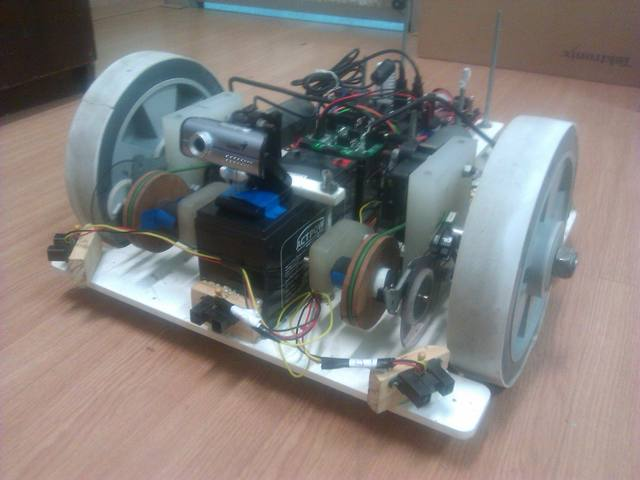
\includegraphics[width=0.9\textwidth]{./figuras/robo/fotos/foto1.jpg}
	%\caption{foto1.}
	\label{fig:robo_foto1}
\end{figure}

\begin{figure}[H]
	\centering
	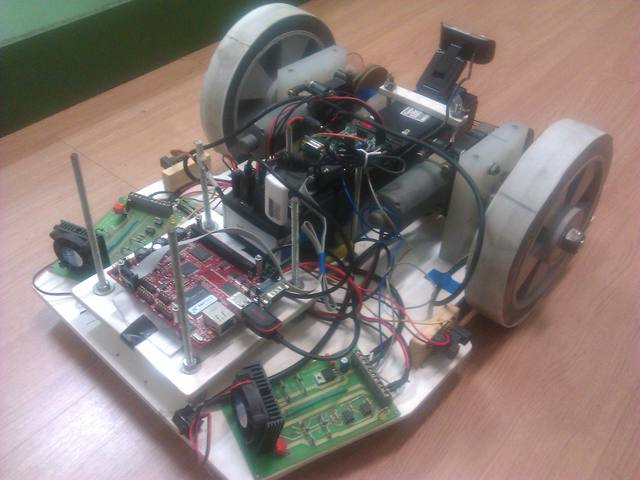
\includegraphics[width=0.9\textwidth]{./figuras/robo/fotos/foto2.jpg}
	%\caption{foto2.}
	\label{fig:robo_foto2}
\end{figure}

\begin{figure}[H]
	\centering
	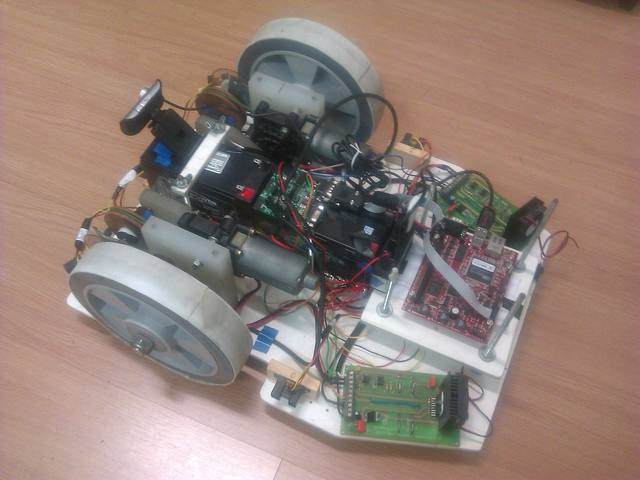
\includegraphics[width=0.9\textwidth]{./figuras/robo/fotos/foto3.jpg}
	%\caption{foto3.}
	\label{fig:robo_foto3}
\end{figure}

\begin{figure}[H]
	\centering
	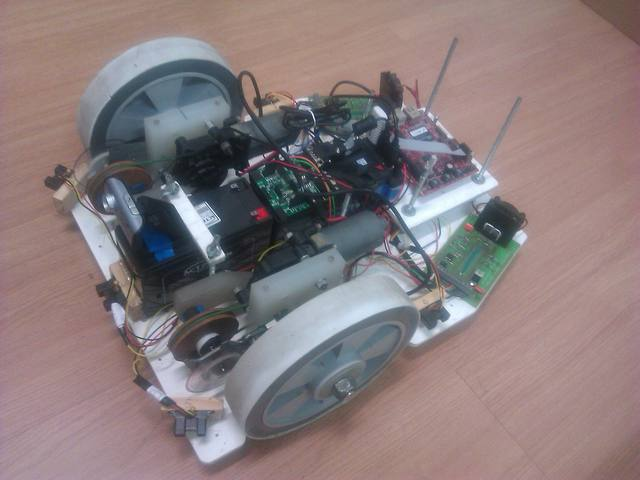
\includegraphics[width=0.9\textwidth]{./figuras/robo/fotos/foto4.jpg}
	%\caption{foto4.}
	\label{fig:robo_foto4}
\end{figure}

\begin{figure}[H]
	\centering
	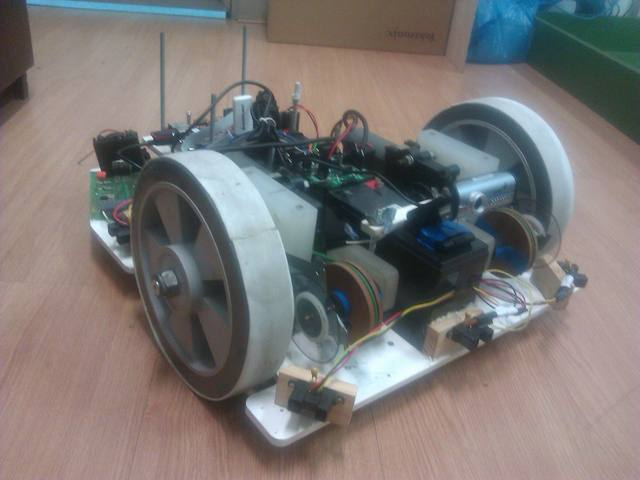
\includegraphics[width=0.9\textwidth]{./figuras/robo/fotos/foto5.jpg}
	%\caption{foto5.}
	\label{fig:robo_foto5}
\end{figure}



\raggedright
\bibliography{referencias}

\end{document}

